\documentclass[]{nsm-thesis}
% options:
% [germanthesis] - Thesis is written in German
% [plainunnumbered] - Don't print numbers on plain pages
% [earlydraft] - Settings for quick draft printouts
% [watermark] - Print current time/date at bottom of each page
% [phdthesis] - switch to PhD thesis style
% [twoside] - double sided
% [cutmargins] - text body fills complete page

% Author name. Separate multiple authors with commas.

\usetikzlibrary{quotes,angles}
\usepackage{nicefrac}
\usepackage{comment}
\usetikzlibrary{shapes, arrows, positioning}
\newcommand{\algorithmautorefname}{Algorithm}
\author{Karl Christian Lautenschläger}
\birthday{29. Juni 1998}
\birthplace{Magdeburg}

% Title of your thesis.
\title{Suitability of Modern Wi-Fi for Wireless-Infield-Communication of Agricultural Machines}

% Choose one of the following lines, changing the word "Computer Science" to match your degree program.
\thesistype{Diploma Thesis in Information Systems Engineering}\thesiscite{Diploma Thesis~(Diplomarbeit)}

\advisors{Christoph Sommer}
% List of advisors (without academic titles), separated by commas.

% List of referees (without academic titles), separated by commas.
\referees{Christoph Sommer, Burkhard Hensel}

\DeclareAcronym{FH}{
	short=FH,
	long=Forage Harvester,
}
\DeclareAcronym{CH}{
	short=CH,
	long=Combine Harvester,
}
\DeclareAcronym{GPS}{
	short=GPS,
	long=Global Positioning System,
}
\DeclareAcronym{STA}{
	short=STA,
	long=station,
}
\DeclareAcronym{IFS}{
	short=IFS,
	long=Interframe Space,
}
\DeclareAcronym{TM}{
	short=TM,
	long=Transport Machine,
}
\DeclareAcronym{BCC}{
	short=BCC,
	long=binary convolutional coding,
}
\DeclareAcronym{RTS}{
	short=RTS,
	long=Request-to-Send,
}
\DeclareAcronym{CTS}{
	short=CTS,
	long=Clear-to-Send,
}
\DeclareAcronym{ER}{
	short=ER,
	long=Extended Range,
}
\DeclareAcronym{MU}{
	short=MU,
	long=Multi-User,
}
\DeclareAcronym{SU}{
	short=SU,
	long=Single-User,
}
\DeclareAcronym{LDPC}{
	short=LDPC,
	long=low-density parity-check,
}
\DeclareAcronym{HT}{
	short=HT,
	long=High-Throughput,
}
\DeclareAcronym{VHT}{
	short=VHT,
	long=Very-High-Throughput,
}
\DeclareAcronym{HE}{
	short=HE,
	long=High-Efficiency,
}
\DeclareAcronym{PER}{
	short=PER,
	long=packet error rate,
}
\DeclareAcronym{BW}{
	short=BW,
	long=Bandwidth,
}
\DeclareAcronym{FEC}{
	short=FEC,
	long=Forward Error Correction,
}
\DeclareAcronym{WPA}{
	short=WPA,
	long=Wi-Fi Protected Access,
}

\DeclareAcronym{DCF}{
	short=DCF,
	long=Distributed Coordination Function,
}
\DeclareAcronym{DIFS}{
	short=DIFS,
	long=Distributed Coordination Function Interframe Space,
}
\DeclareAcronym{SSID}{
	short=SSID,
	long=Service Set Identifier,
}
\DeclareAcronym{SIFS}{
	short=SIFS,
	long=Short Interframe Space,
}
\DeclareAcronym{ACK}{
	short=ACK,
	long=Acknowledgement,
}
\DeclareAcronym{NAV}{
	short=NAV,
	long=Network Allocation Vector,
}
\DeclareAcronym{PCF}{
	short=PCF,
	long=Point Coordination Function,
}
\DeclareAcronym{CSMACA}{
	short=CSMA/CA,
	long=Carrier Sense Multiple
	Access/Collision Avoidance,
}

\DeclareAcronym{IBSS}{
	short=IBSS,
	long=Independent Basic Service Set,
}
\DeclareAcronym{AP}{
	short=AP,
	long=Access Point,
}
\DeclareAcronym{PD}{
	short=PD,
	long=Plant Density,
}
\DeclareAcronym{WIC}{
	short=WIC,
	long=Wireless Infield Communication,
}
\DeclareAcronym{M2M}{
	short=M2M,
	long=Machine-To-Machine,
}

\DeclareAcronym{MIMO}{
	short=MIMO,
	long=Multiple Input Multiple Output,
}
\DeclareAcronym{STBC}{
	short=STBC,
	long=Space-Time-Block-Code,
}
\DeclareAcronym{PPDU}{
	short=PPDU,
	long=Physical layer convergence protocol data unit,
}
\DeclareAcronym{MCS}{
	short=MCS,
	long=Modulation
	and Coding Scheme,
}
\DeclareAcronym{CR}{
	short=CR,
	long=Coding Rate,
}
\DeclareAcronym{GI}{
	short=GI,
	long=Guard Interval,
}
\DeclareAcronym{DCM}{
	short=DCM,
	long=Dual Carrier Modulation,
}
\DeclareAcronym{MANET}{
	short=MANET,
	long=Mobile Ad Hoc Network
	and Coding Scheme,
}  

\DeclareAcronym{ASC}{
	short=ASC,
	long=Automatic Section Control,
}
\DeclareAcronym{m-ASC}{
	short=m-ASC,
	long=Meshed Automatic Section Control,
}
\DeclareAcronym{AEF}{
	short=AEF,
	long=Agricultural Industry Electronics Foundation,
}
\DeclareAcronym{FMIS}{
	short=FMIS,
	long=Farm Management Information System,
}
\DeclareAcronym{hTMM}{
	short=hTMM,
	long=Hybrid Threat Modeling Method,
}


\DeclareAcronym{UDP}{
	short=UDP,
	long= User Datagram Protocol,
}

\DeclareAcronym{OFDMA}{
	short=OFDMA,
	long= Orthogonal Frequency-Division Multiple Access,
}
\DeclareAcronym{OFDM}{
	short=OFDM,
	long= Orthogonal Frequency-Division Multiplexing,
}
\DeclareAcronym{RU}{
	short=RU,
	long= Resource Unit,
}
\DeclareAcronym{SINR}{
	short=SINR,
	long= Signal-to-Interference-plus-Noise Ratio,
}
\DeclareAcronym{QAM}{
	short=QAM,
	long=Quadrature Amplitude Modulation,
}
\DeclareAcronym{PSK}{
	short=PSK,
	long=Phase Shift Keying,
}
\DeclareAcronym{RSS}{
	short=RSS,
	long=Received Signal Strength,
}
\DeclareAcronym{LOS}{
	short=LOS,
	long=Line-Of-Sight,
}
\DeclareAcronym{SNR}{
	short=SNR,
	long=Signal Noise Ratio,
}
\DeclareAcronym{PDR}{
	short=PDR,
	long=Packet Delivery Ratio,
}

\DeclareAcronym{ESS}{
	short=ESS,
	long=Extended Service Set,
}
\DeclareAcronym{BSS}{
	short=BSS,
	long=Basic Service Set,
}
\DeclareAcronym{V2X}{
	short=V2X,
	long=Vehicle-to-everything,
}
\DeclareAcronym{EDCA}{
	short=EDCA,
	long=Enhanced Distributed Channel Access,
}



% Define abbreviations used in the thesis here.
\acrodef{WSN}{Wireless Sensor Network}

\acrodef{ROI}{Region of Interest}{short-indefinite={an}, long-plural-form={Regions of Interest}}
\acrodef{ADAC}{German Automobile Association}{foreign={Allgemeiner Deutscher Automobilclub}}
\acrodef{CANhashing}[CAN]{Content Addressable Network}{extra={when referring to the distributed hash table}}
\acrodef{CANproto}[CAN]{Controller Area Network}{extra={when referring to the bus protocol}}

\begin{document}

\pagenumbering{roman}

\maketitle

\cleardoublepage

\chapter*{Abstract}
\addcontentsline{toc}{chapter}{Abstract}
\begin{otherlanguage*}{american}

\begin{comment}
    about 1/2 page:
\begin{enumerate}
    \item Motivation (Why do we care?)
    \item Problem statement (What problem are we trying to solve?)
    \item Approach (How did we go about it)
    \item Results (What's the answer?)
    \item Conclusion (What are the implications of the answer?)
\end{enumerate}

The abstract is a miniature version of the thesis.
It should be treated as an entirely separate document.
Do not assume that a reader who has access to an abstract will also have access to the thesis.
Do not assume that a reader who reads the thesis has read the abstract.

\end{comment}

\ac{WIC} describes a wireless data exchange between agricultural machines in the field.
A prototypical use case is an Agricultural Platooning Service, which exchanges guidance data positions following
vehicles in a platoon with a lateral and longitudinal offset to a leading vehicle in the field.
This thesis investigates the suitability of modern Wi-Fi for \ac{WIC} based on the use case Agricultural Platooning Service.
I analyzed process data and derived requirements of Agricultural Platooning Services in the the corn harvest scenario.

Field measurements in an agricultural environment indicated that Wi-Fi communication can range up to \SI{2500}{\metre} in
a line-of-sight scenario.
However, signal strength can suffer from multipath, shadowing and fading effects due to the
agricultural environment and the machine sizes.


I simulated different Wi-Fi physical layer configurations that reduce the data rate but
enable robust communication to overcome these challenges.
The results enable configuration for long-range service discovery and uniform guidance data exchange modes
in the Agricultural Platooning Service.
Finally, it was shown that the required latencies and message intervals for Agricultural Platooning Services could be met in the corn harvest
scenario.

\end{otherlanguage*}

\chapter*{Kurzfassung}
\addcontentsline{toc}{chapter}{Kurzfassung}
\begin{otherlanguage*}{ngerman}


\acf{WIC} beschreibt den drahtlosen Datenaustausch zwischen landwirtschaftlichen Maschinen auf dem Feld.
Ein prototypischer Anwendungsfall sind elektronische Deichseln in der Landwirtschaft, die Positionierungsdaten austauschen, um nachfolgender
Fahrzeuge eines Zuges mit einem latitudinalen und longitudinalen Versatz zu einem führenden Fahrzeug im Feld zu führen.
In dieser Arbeit wurde die Eignung von modernem Wi-Fi für \ac{WIC} anhand dieses Anwendungsfalls untersucht.
Ich analysierte Prozessdaten und leitete daraus Anforderungen für die Anwendung von elektronischen Deichseln in der Maisernte ab.

Feldmessungen in einer landwirtschaftlichen Umgebung ergaben, dass die Wi-Fi-Kommunikation bei Sichtverbindung eine Reichweite von bis zu \SI{2500}{\metre}
möglich ist.
Die Signalstärke kann jedoch aufgrund der landwirtschaftlichen Umgebung und der Größe der Maschinen unter Mehrwegeffekten, Abschattungen und Pfadverlusten leiden.
landwirtschaftlichen Umgebung und der Größe der Maschinen leiden.

Ich habe verschiedene Wi-Fi Konfigurationen der physikalischen Schicht simuliert, die die Datenrate reduzieren, aber
robuste Kommunikation ermöglichen, um diesen Herausforderungen zu begegnen.
Die Ergebnisse ermöglichen eine Konfiguration für den Broadcast des Dienstes über große Entfernungen und den uniformen Austausch von
Positionierungsdaten für die elektronische Deichsel in der Landwirtschaft.
Schließlich konnte gezeigt werden, dass die erforderlichen Latenzen und Nachrichtenintervalle für landwirtschaftliche Platooning-Dienste in einem Maisernte
Szenario eingehalten werden können.

\end{otherlanguage*}
\acresetall



\cleardoublepage



\tableofcontents

\cleardoublepage
\pagenumbering{arabic}


\chapter{Introduction}
%\chapter{Einleitung}
\label{sec:introduction}
\todo[color=blue]{Den Teil haben mehrere Leute Korrektur gelesen, sodass du den für den Verständnis auch nur überfliegen kannst.}
\begin{itemize}
\item general motivation for your work, context and goals.
\item context: make sure to link where your work fits in
\item problem: gap in knowledge, too expensive, too slow, a deficiency, superseded technology
\item strategy: the way you will address the problem
\item recommended length: 1-2 pages.
\end{itemize}
With the growing demand for increased efficiency and autonomy in the agricultural domain, \ac{WIC} has emerged as a key technology to improve the automation
and digitalization of farming processes. \ac{WIC} describes a wireless connection between agricultural machines
in the field that enables process data exchange.

Given that there are many agricultural technology companies worldwide, and a mix of their machines often cooperate in individual agricultural companies, demand for interoperability between agricultural machines of other brands
has emerged.
In 2008, the \ac{AEF} was founded to develop and standardize this interoperability
\footnote{\url{https://www.aef-online.org/about-us/about-the-aef.html}}.

The AEF is known fot its developed binary unit system, the ISO 11783 standard, for agricultural machinery communication, mainly tractors and
implements \cite{iglesias_enabling_2014}.
According to \textcite{schlingmann_aef_2019}, the ISO 11783 standard is named ISOBUS system.

The authors mention that the AEF is currently working on other issues.
Among them is also \ac{WIC}.
The associated project group \ac{WIC} develops and standardizes solutions for \ac{M2M} wireless
communication between cooperating agricultural machines.

In order to implement \ac{WIC}, the \ac{WIC} project group has been searching for a suitable technology
that can realize the required data rates, latencies, robustness, and high transmission range.
The plans to implement \ac{WIC} are written down by members of the \ac{WIC} project group in \cite{schlingmann_challenges_2017}.
The authors consider the fundamental use of cellular networks as very problematic
because, according to \cite{itu2016facts}, only \SI{30}{\percent} of the land surface has network coverage.
For this reason, one major concern is that the required data cannot be exchanged because there is
no network connectivity around many fields.
Nevertheless, the authors want to leave the future \ac{WIC} system open
to cellular standards.

The authors' current focus is on Wi-Fi technologies, especially IEEE 802.11p.

As of July 2021, the frequency spectrum of IEEE 802.11p in the United States of
America, ranging from \SIrange{5.85}{5.925}{\giga\hertz}, has been split.
The upper \SI{30}{\mega\hertz}
are reserved for Intelligent transportation systems now.
The lower \SI{45}{\mega\hertz} have
been released for unlicensed operations \cite{fcc_use_2021}. \todo[color=yellow]{andere Länder Japan, Korea?}

Since the use of IEEE 802.11p has now been partly limited by the  US Federal Communications Commission, the
WIC project group is looking for an alternative Wi-Fi technology that enables \ac{WIC}.

In my final thesis, I intend to support the progress of the \ac{WIC} project group and investigate how modern Wi-Fi can enable \ac{WIC}.
 In particular, I will focus on the current Wi-Fi standard, IEEE 802.11ax.
During my research, I will study the use cases of \ac{WIC} in agriculture and the requirements and challenges for \ac{WIC} in agriculture.
To analyze the suitability of IEEE 802.11ax to enable \ac{WIC}, I will concentrate on the example use case Agricultural Platooning Service.
Agricultural Platooning Service enables the exchange of process data
to guide a vehicle in a platoon with a lateral and longitudinal offset to a leading vehicle.

In the beginning, I will analyze agricultural process data to find the requirements and challenges of the mentioned use case.
I will complement these with insights from past research on \ac{WIC} in agriculture and wireless technologies
in the agriculture domain in general.

The suitability of IEEE 802.11ax for \ac{WIC} depends on whether the required data rates, latencies, robustness, high
transmission ranges and robustness in the harsh agricultural environment can be achieved.

By understanding past limitations of Wi-Fi technologies for outdoor communication networks
and exploring how IEEE 802.11ax addresses these limitations, I will investigate how IEEE 802.11ax can be configured.
For this purpose, I will first simulate how the capabilities of IEEE 802.11ax affect the data rate and the robustness of the wireless connection.
After learning suitable parameter settings for the physical and MAC layer of IEEE 802.11ax, I will simulate the use case
Agricultural Platooning Service to determine whether the requirements and challenges
can be met by IEEE 802.11ax.


\todo{Add Field experiments to the thesis plan.}

\chapter{Fundamentals}
\label{sec:fundamentals}


\section{\acl{WIC}}

\todo[color=blue]{Den Teil haben mehrere Leute Korrektur gelesen. Den musst du nicht überfliegen, da man ihn kaum für das Verständnis braucht.}
Since 2014, the \ac{WIC} project group has been working on the development of a for \ac{WIC} standard, which covers a standard for machine-to-machine communication, encryption, and security \footnote{https://www.aef-online.org/about-us/teams.html}.
\textcite{schlingmann_aef_2019} summarize the goals of the \ac{WIC} project team as follows:
\begin{itemize}
	\item Define use cases for \ac{WIC} in agriculture
	\item Evaluate the suitability of communication technologies
	\item Find suitable communication protocols
	\item Standardize the \ac{WIC} common software library
	\item Develop functional and security requirements and concepts
	\item Test first prototypes in regards of cross-brand comformance
	\item Write a application guideline
\end{itemize}
First steps have already been taken in this direction. The use cases and key scenarios are defined and explained by the authors as follows:
\begin{itemize}
	\item \textbf{Real-Time Machine-to-Machine Control} is the exchange of control data under real-time conditions with defined latency policies. This use case enables leader-follower scenarios where agricultural machines follow a leading agricultural machine at a lateral and longitudinal distance. Throughout this thesis, I will refer to Real-Time Machine-to-Machine Control as Agricultural Platooning Service.
	%\TODO{Fendt-Paper? Auch erwähnen eigentlich ja später, Beispiel aus AEF Paper?}
	\item \textbf{Streaming Services} are communications that stream video from remote cameras and monitors at a high data rate and low latency. The authors estimate the distance between the communication participants to be less than \SI{100}{\metre}. As a result, this data is available on another agricultural vehicle and can be analyzed and processed there.
	I will refer to Streaming Services as Agricultural Streaming Services in this thesis. %\TODO{Camera harvest streaming}
	\item \textbf{Process Data Exchange} describes the exchange of process data. One example is the exchange of already sprayed field areas to prevent multiple spraying of fertilizers and pesticides on the same field area by different machines. According to the authors, this \ac{WIC} use case requires long-range technologies because agricultural fields worldwide can be vast.
	%\TODO{ISO 11783-10 extended FMIS Data Interface}
	\item \textbf{Fleet Management \& Logistics} is the potential retrieval of data from the ongoing agricultural process. This information can influence economic or agronomic decisions of agricultural enterprises or service companies and is therefore required in a \ac{FMIS}.
	Since not all agricultural machines may be connected to the \ac{FMIS}, the \ac{WIC} project group is looking at how to use \ac{M2M} communications to bridge the missing communications infrastructure until the data reaches a machine that can connect to the \ac{FMIS}.
	\item \textbf{Road Safety} describes a use case which is already a project between the European Telecommunication Standard Institute and the \ac{AEF}. Since agricultural vehicles are repeatedly underestimated in their size and speed by other road users when they suddenly turn off the field onto the road, the other road users need to be warned in this situation. In this way, smart technologies in cars and motorcycles can brake these vehicles in advance and prevent possible accidents.
\end{itemize}

\todo[color=blue]{Wichtig:}
Considering that I investigate the Suitability of modern Wi-Fi for Wireless-Infield-Communication and modern Wi-Fi like IEEE 802.11ax is no long range technologies,
I will focus on investigating the suitability of IEEE 802.11ax for the \ac{WIC} use case Real-Time Machine-to-Machine Control.
Throughout this thesis, I will refer to real-time machine-to-machine control as Agricultural Platooning.
An example how farmers can benefit from Streaming Services or Agricultural Platooning Services is the corn harvesting and loading process.


\section[Use Cases for \acl{WIC}]{Harvest and Loading Processes as Use Cases for \acl{WIC}}
\label{sec:corn_harvest_scenario}
The Forage harvester has proven to be an essential agricultural machine for harvesting and loading forage. \textcite{seifert_feldhacksler_1962} define a forage harvester
as an agricultural loading machine for nearly all types of animal feed. According to the authors, a forage harvester can load the following animal feed by mounting different cutting and loading devices: Hey, Straw, Corn, Grass and Clover.
\begin{figure}%
	\centering
	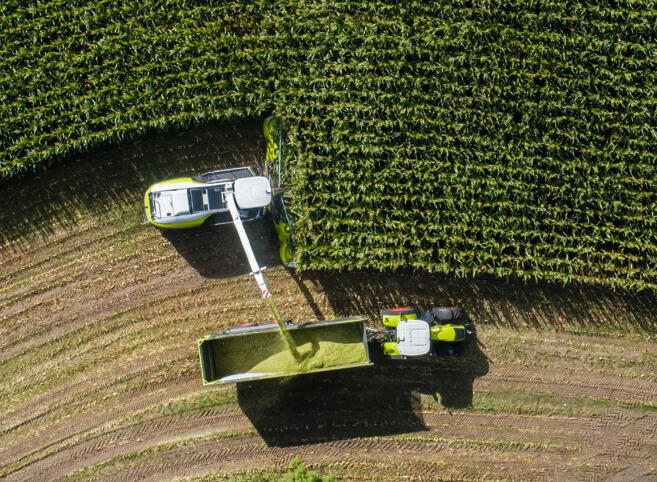
\includegraphics[width=0.6\textwidth]{figures/claas_harvest_side.png}
	\caption{\acf{FH} and \acf{TM} in a corn harvesting and loading process}%
	\label{fig:normal}%
\end{figure}

In the harvesting and loading process, a \ac{TM} typically drives alongside or behind the \ac{FH} so that the \ac{FH} can load the harvested goods onto the trailer of the \ac{TM} using the spout. Drivers operate both machines and try to keep the speed and distance so that the spout only throws the harvested goods into the trailer of the TM. An image of a corn harvesting and loading process can be seen in \autoref{fig:normal}.

Taking a corn harvest scenario as an example, some key figures are represented in \cite{faustzahlen2018}, a standard reference book in agricultural literature. This book contains key figures of agricultural processes, which 80 experts have compiled.
The key figures, which are shown in \autoref{tab:DataSilageHarvest}, are dependent on the \ac{PD} and show the large amount of forage harvested by a \ac{FH} every hour.
\begin{table}[H]
	\centering
	\begin{tabular}{>{\raggedright}p{4.9cm}p{1.8cm}p{1.8cm}p{1.8cm}}
		\toprule
  		\acf{PD}&\SI{20}{\tonne\per\hectare}&\SI{30}{\tonne\per\hectare} & \SI{50}{\tonne\per\hectare}\\
		\midrule
		Required \acl{TM}s & \num{5}&
		\num{7} & \num{10} \\
		Harvested volume in \si{\cubic\metre\per\hour} &
		\num{285.7}-\num{333.3}
		& \num{428.6}-\num{500.0} &
		\num{595.7}-\num{695.0}\\
		Filled \acl{TM} loads in \si{\per\hour} &
		\num{5.7} - \num{6.7}
		& \num{8.6} - \num{10.0} &
		\num{11.9} - \num{13.9}\\
		Harvested mass in \si{\tonne\per\hour} & \num{100}
		& \num{150} &
		\num{208.5} \\
		\bottomrule
	\end{tabular}
	\caption{Key figures of corn harvest of a \acf{FH} with a working width of \SI{6.2}{\metre} in a \SI{80}{\hectare}-field in regards to \acf{PD}  \cite{faustzahlen2018}}
	\label{tab:DataSilageHarvest}
\end{table}

The harvesting and loading processes are examples of the use of agricultural Platooning Services as described by
\textcite{zhang_method_2009}.
This Platooning Service creates a leader and follower system where an uncrewed agricultural machine follows a leading operated agricultural machine.
The operated \ac{FH}, as a leader, sets the path and speed and transmits the data via \ac{WIC} to the \ac{TM}. Based on the path and speed data of the \ac{FH}, \ac{TM} follows unmanned with a longitudinal and lateral offset, as \autoref{fig:offset} displays.
\begin{figure}[H]
	\centering
	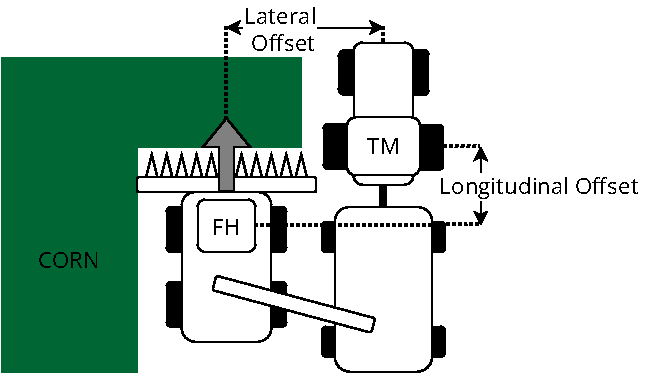
\includegraphics[width=0.65\textwidth]{figures/offset_platoon.pdf}
	\caption{Lateral and longitudinal offset between the two agricultural machines \acf{FH} and \acf{TM} in a corn harvest scenario}%
	\label{fig:offset}%
\end{figure}

The application of platooning services offers many advantages.
The \ac{TM} is positioned optimally to the \ac{FH} so that the forage can be loaded ideally from the \ac{FH} onto the \ac{TM}.

Because, as displayed in \autoref{fig:workforce_agri}, fewer and fewer workers are working in agriculture, platooning services for harvest and loading processes can save and free up labour for other activities \cite{liu_automation_2022}. As stated in \autoref{tab:DataSilageHarvest}, ten drivers for the \ac{TM}s are needed in the corn harvest process with a high \ac{PD}. Using an agricultural Platooning Service, each \ac{TM} can drive unmanned in the field, leading to fewer workers needed in the corn harvest process.

\begin{figure}[H]
	\centering
	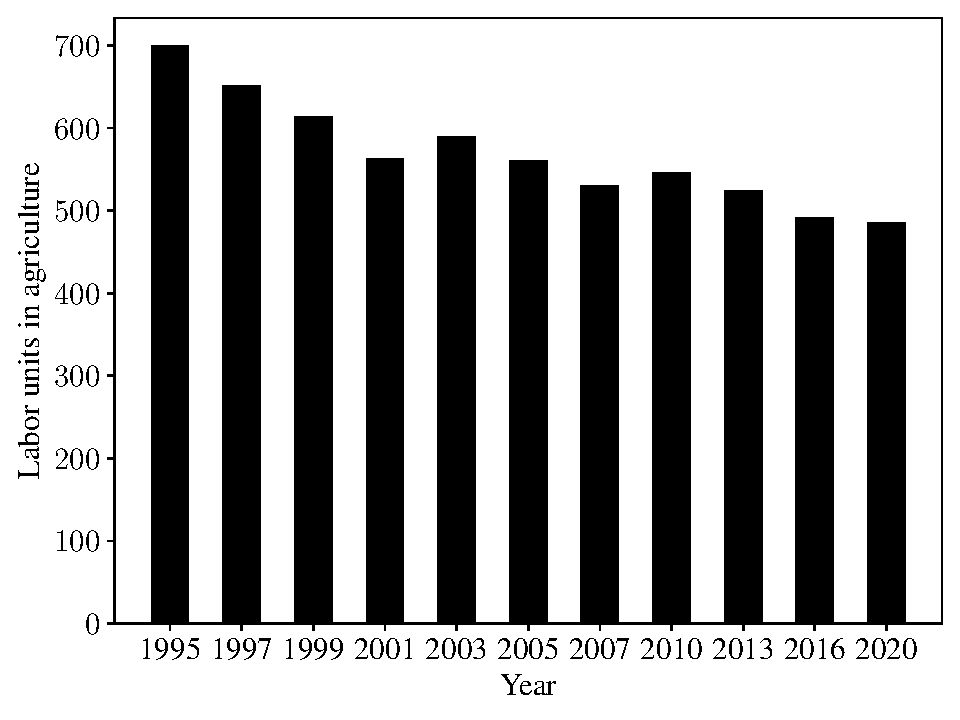
\includegraphics[width=0.75\textwidth]{figures/WorkForceAgriculture.pdf}
	\caption{Decrease in the agricultural labor force in Germany based on the data from \cite{bmel2020}}%
	\label{fig:workforce_agri}%
\end{figure}

\textcite{smolnik_5g_2020} adds that platooning services at the platoon level can reduce \ac{FH} drivers' workload so that they can focus on optimally adjusting the machines.
In addition, \ac{TM}s can be guided to the \ac{FH}s in a targeted manner so that logistics processes in the field can be improved.

At the same time, the harvest and loading processes are examples of the video streaming \ac{WIC} use case, where a video of the \ac{TM}'s filllevel is available at the \ac{FH} and could be transmitted to the \ac{TM} in order to inform the \ac{TM} driver about the machines filllevel. During these harvest and loading processes, the spout of the \ac{FH} must be controlled to set the loading position of the forage into the trailer of the \ac{TM}.

According to \textcite{murcia_quadrotor_2014}, different spout guidance and control systems have been developed to automate the filling of the trailer. Spout guidance and control systems use a camera attached to the spout to determine the fill volume at each point of the trailer via machine vision and set the spout to fill the empty parts accordingly. The author describes Autofill - systems from Claas and Intellifill - systems from CNH Industrial as examples of spout guidance systems.

Streaming the video of a camera at the spout from the \ac{FH} to the \ac{TM} would be a practical application of the video streaming use case in the harvesting process. If the \ac{TM} driver can watch a live stream of the trailer's fill level, he will always be
informed and knows when the trailer is full and can drive the forage back to the
farm.



\section{Wireless Lans according to IEEE 802.11}


According to \textcite[41]{kauffels_wireless_2002}, the first version of the Standard IEEE 802.11 was published in 1999 to enable a wireless alternative to Ethernet - or Token-Ring - networks.
\textcite[265-268]{sauter_wireless_2022} considers IEEE 802.11 also to be an implementation of Ethernet with the help of wirless radio technologies.
The author lists the extensions to the original standard, which range from 802.11b, 802.11g, 802.11a, 802.11n, 802.11ac to the latest enhancement 802.11ax. The different IEEE 802.11 standards can operate in the  \SI{2.4}{\giga\hertz} - , \SI{5}{\giga\hertz} and \SI{6}{\giga\hertz} - frequency band.
IEEE 802.11n is also known as \ac{HT} Wi-Fi \cite{ieee_standard_2009n}, IEEE 802.11ac as \ac{VHT} Wi-Fi \cite{ieee_standard_2020} and IEEE 802.11ax as \ac{HE} Wi-Fi \cite{ieee_standard_2021ax}.
The standards are acknowledged by these names.
In addition, they are also called Wi-Fi 4, Wi-Fi 5 and Wi-Fi 6 respectively.
\textcite{jacob_system-level_2020} adds that there are also two extensions IEEE 802.11p and its successor IEEE 802.11bd. These operate in a reserved frequency spectrum for \ac{V2X} according to the authors in the \SI{5.9}{\giga\hertz} frequency spectrum.

\textcite[42,43,178-180]{kauffels_wireless_2002} defines the following three basic architectures for IEEE 802.11.

If two or more \acp{STA} communicate directly without an \ac{AP}, they form an ad hoc network.
According to the author, this can be set up quickly and easily and is called \ac{IBSS}.

The Infrastructure \ac{BSS} mode allows all \ac{STA}s within the range of defined range around the \ac{AP} to communicate via a central \ac{AP}. Within the area of the \ac{BSS}, all stations can move freely and communicate with one another.

Since an \ac{AP} has limited range and can only cover a certain area, the \ac{ESS} was introduced.
It contains a distribution system, which links several \ac{BSS} with each other.

Thereby, the BSS coverage areas can physically overlap so that continuous connection of stations within the ESS can be provided.
For a better performance the \ac{BSS} can be physically placed on top of each other.
One can also have objectively separate \ac{BSS}s so that these \ac{BSS}s can be linked together over long distances.
According to the author, the standard does not specify a distance limit for such connections.

He also mentions that the standard defines the following three mobility types for station in an \ac{ESS}, where a station can do no-transition and thereby stay within a \ac{BSS}, \ac{BSS}-transitioning and move from one \ac{BSS} to another \ac{BSS} within the same \ac{ESS} and \ac{ESS}-transition, where the Station moves from an \ac{ESS} to another one but no stable connection can be guaranteed.

\textcite[272, 273]{sauter_wireless_2022} adds that usually Ethernet is used to link \ac{AP}s within an \ac{ESS}.
But according to the author this can be replaced by a wireless connection, which is called wireless bridge.

To enable communication between Wi-Fi devices, the IEEE 802.11 standard defines the physical and the MAC layer of the OSI model. The first layer is the physical layer.


\subsection*{Wi-Fi Physical Layer}
A constant change of the physical layer accompanies the further development of IEEE 802.11.
\textcite{sauter_wireless_2022} mentions that all new enhancements of the physical layer of IEEE 802.11 are backward
compatible with previous definitions of the standard.

According to the Author, IEEE 802.11 initially used DSSS and FHSS as modulation methods.
Since IEEE 802.11g the modulation method \ac{OFDM} can be used in the \SI{2.4}{\giga\hertz} frequency band.
The author explains \ac{OFDM} as follows. \ac{OFDM} divides the transmission channel into subcarriers with different
amplitudes, frequencies and phases.
Each subcarrier is orthogonal to another one, as they send the information ``Low``,
where only one other subcarrier is sending the information ``High``.


\subsubsection*{Symbol length}
The data is then sent as \ac{OFDM} symbols over the individual \ac{OFDM} subcarriers.
The distance between the ``Highs`` of the subcarriers is specified as subcarrier spacing and corresponds to the reciprocal
symbol length.
IEEE 802.11ax increased the \ac{OFDM} symbol length from \SI{3.2}{\micro\second} for IEEE 802.11n to a maximum of \SI{12.8}{\micro\second} \cite{sauter_wireless_2022}.
This corresponds to a subcarrier spacing of \SI{312.5}{\kilo\hertz} and \SI{78.125}{\kilo\hertz} respectively \cite{sauter_wireless_2022}.

For the IEEE 802.11p and IEEE 802.11bd standards, a symbol length of \SI{6.4}{\micro\second} applies, corresponding to a subcarrier spacing of \SI{156.25}{\kilo\hertz} \cite{jacob_system-level_2020}.

The Fast Fourier Transform and Inverse Fast Fourier Transform are used to modulate and demodulate the transmitting bits.
With the reduction of subcarrier spacing, more subcarriers are created in the transmission channel,
so the Fast Fourier Transform size must be increased.

\textcite{kauffels_wireless_2002} adds that \ac{OFDM} can be used in the \SI{5}{\giga\hertz} frequency band since IEEE 802.11a.
\subsubsection*{\acf{BW}}
The frequency bands are divided into channels in order to create several transmission channels.
This results in 13 channels in Europe in the frequency band of \SIrange{2.412}{2.482}{\giga\hertz} and 18 channels in the frequency band of \SIrange{5.180}{5.350}{\giga\hertz} and \SIrange{5.180}{5.350}{\giga\hertz} \cite{sauter_wireless_2022}.
Transmission channels can be combined to enable higher data rates.
Every channel has a width called \ac{BW} specified in \si{\mega\hertz}.
The possible \ac{BW}s for the IEEE 802.11 standards are shown in \autoref{tab:BW}.
\begin{table}[!ht]
	\centering
	\begin{tabular}{>{\raggedright}p{2.2cm}p{2.50cm}p{2.55cm}p{2.50cm}}
		\toprule
		Standard & Channel \ac{BW}s\newline in \SI{2.4}{\giga\hertz}& Channel \ac{BW}s\newline in \SI{5}{\giga\hertz} &  Channel \ac{BW}s\newline in  \SI{5.9}{\giga\hertz}\\
		\midrule
		IEEE 802.11n \cite{sauter_wireless_2022}& \SI{20}{\mega\hertz},\SI{40}{\mega\hertz}  & \SI{20}{\mega\hertz},\SI{40}{\mega\hertz} & - \\
		\midrule
		IEEE 802.11ac \cite{noauthor_ieee_2021-1}& -  & \SI{20}{\mega\hertz},\SI{40}{\mega\hertz}, \SI{80}{\mega\hertz},\SI{160}{\mega\hertz} & - \\
		\midrule
		IEEE 802.11ax \cite{noauthor_ieee_2021}&\SI{20}{\mega\hertz},\SI{40}{\mega\hertz}  & \SI{20}{\mega\hertz},\SI{40}{\mega\hertz}, \SI{80}{\mega\hertz},\SI{160}{\mega\hertz} & - \\
		\midrule
		IEEE 802.11p \cite{jacob_system-level_2020}& - & - & \SI{10}{\mega\hertz} \\
		\midrule
		IEEE 802.11bd \cite{jacob_system-level_2020}& - & - & \SI{10}{\mega\hertz},\SI{20}{\mega\hertz} \\
		\bottomrule
	\end{tabular}
	\caption{Available \ac{BW}s for the IEEE 802.11 standards per frequency band.}
	\label{tab:BW}
\end{table}

IEEE 802.11ac and IEEE 802.11ax also enable the use of a discontinuous \ac{BW}, which combines two \SI{80}{\mega\hertz}
channel to a \SI{160}{\mega\hertz} \ac{BW} channel \cite{noauthor_ieee_2021}, \cite{noauthor_ieee_2021-1}.

While wider channels increase the theoretical data rate, \textcite{avallone_will_2021} mentions that narrower channels can
boost the signal's power spectral density and thus increase the transmission range.

\subsubsection*{\acf{MCS}}

In order to encode as many bits as possible on one \ac{OFDM} symbol, different \ac{MCS}s can be used.
The \ac{MCS}s for the IEEE 802.11 standards are based on \ac{PSK} or \ac{QAM}. \cite{kauffels_wireless_2002}.
The smallest \ac{MCS} is Binary - \ac{PSK} and encodes \SI{1}{\bit} per symbol.
IEEE 802.11ax has the most complex \ac{MCS} of \num{256} - \ac{QAM} IEEE 802.11ac to \num{1024} - \ac{QAM} and thus now encodes \SI{10}{\bit} per symbol \cite{afaqui_ieee_2017}.
In the \ac{V2X} standards IEEE 802.11p and IEEE 802.11bd, the \ac{MCS}s can range from binary - \ac{PSK} to \num{256} - \ac{QAM} \cite{jacob_system-level_2020}.

An imaginary, theoretical transmission channel is usually specified as a square-wave signal in the frequency domain
with limits of both minimum and maximum amplitude and cut-off frequency. \textcite{kauffels_wireless_2002} defines
the roll-off factor as a cosine-shaped flattening of the square signal between 0 and 1.
In addition, the author points
out that \ac{QAM} can generate high roll-off factors so that signals interfere significantly more with adjacent channels.

In this regard, the author recommends setting the parameters in an \ac{OFDM} system so that first, the coding
rate and then the complexity of the \ac{MCS} is reduced in challenging transmission environments. The more bits a \ac{MCS} encodes
on a symbol, the more error-prone the correct decoding.

\subsubsection*{\acf{FEC}}

Nevertheless, bit errors can occur during transmission. In this regard, \cite{kauffels_wireless_2002}
mentions and explains \ac{FEC} as a technique to reduce bit errors during transmission. \ac{FEC} adds redundant bits
to the data. The receiver uses these redundant bits to check the integrity or correct errors of the received data.
The proportion of non-redundant transmission bits is defined in the \ac{CR}.

To achieve this, \ac{BCC} is used mandatory since the IEEE 802.11n standard \cite{afaqui_ieee_2017,syafei_performance_2009}
. \textcite{syafei_performance_2009} add that it is optionally possible to
use \ac{LDPC}.
The authors state that \ac{LDPC} can achieve a better channel capacity performance.
This impact is also confirmed by \textcite{afaqui_ieee_2017}, who point out that \ac{LDPC} also generates higher computational cost.

IEEE 802.11ax stations must support \ac{LDPC} when using the IEEE 802.11ax standard under
the following conditions \cite{afaqui_ieee_2017,noauthor_ieee_2021} :
\begin{itemize}
   \item The used bandwidth is greater than \SI{20}{\mega\hertz}
   \item The chosen \ac{MCS} is \num{1024}-\ac{QAM}
   \item More than four transmission channels are used for the transmission.
\end{itemize}
IEEE 802.11ax achieves \ac{CR} of \nicefrac{1}{2}, \nicefrac{2}{3}, \nicefrac{3}{4}, and \nicefrac{5}{6} \cite{noauthor_ieee_2021}.
Similarly, IEEE 802.11p uses the \ac{BCC} technique, which has been superseded by \ac{LDPC} in its successor
IEEE 802.11ax \cite{jacob_system-level_2020,krief_analysis_2020}.
\textcite{krief_analysis_2020} argue that this step was important, as \ac{LDPC} offers better error correction
possibilities for higher communication ranges greater than \SI{50}{\metre}.

Together with the \ac{MCS}, the \ac{FEC} \ac{CR} form a physical layer specification, which is named after the specific standard.
For IEEE 802.11ax, this results in the HE-MCS values in \autoref{tab:HEMCS}.

\begin{table}[!ht]
   \centering
   \begin{tabular}{>{\raggedright}p{2cm}p{3cm}p{2cm}}
      \toprule
      HE-MCS index & \acf{MCS} & \acf{CR} \\
      \midrule
      \num{0} & Binary \ac{PSK}& \nicefrac{1}{2}\\
      1 & Quadrature \ac{PSK}& \nicefrac{1}{2}\\
      2 & Quadrature \ac{PSK}& \nicefrac{3}{4}\\
      3 & \num{16}-\ac{QAM}& \nicefrac{1}{2}\\
      4 & \num{16}-\ac{QAM}& \nicefrac{3}{4}\\
      5 & \num{64}-\ac{QAM}& \nicefrac{2}{3}\\
      6 & \num{64}-\ac{QAM}& \nicefrac{3}{4}\\
      7 & \num{64}-\ac{QAM}& \nicefrac{5}{6}\\
      8 & \num{256}-\ac{QAM}& \nicefrac{3}{4}\\
      9 & \num{256}-\ac{QAM}& \nicefrac{5}{6}\\
      10 & \num{1024}-\ac{QAM}& \nicefrac{3}{4}\\
      11 & \num{1024}-\ac{QAM}& \nicefrac{5}{6}\\
      \bottomrule
   \end{tabular}
   \caption{\ac{MCS} and \ac{CR} for HE-\ac{MCS} values \cite{noauthor_ieee_2021}}
   \label{tab:HEMCS}
\end{table}

\begin{comment}
	{Wellenausbreitung, Überlagerungseffekte, Reflexsion, Reflexsion nicht bei Metall}

\end{comment}

\subsubsection*{\acf{GI}}
\textcite{pulimamidi_development_2007} describe the Guard Interval as a cyclic prefix of \ac{OFDM} symbols to prevent
intersymbol interference and through intercarrier interference.
Intersymbol interference is caused by multipath delays, where the reflected delayed previous symbol can interfere
with the currently received symbol\cite{ravindranath_performance_2016}.
Similarly, intercarrier interference is caused by time-varying channel resulting in a longer \ac{OFDM} symbol duration
\cite{van_duc_nguyen_intercarrier_2002}.


\textcite{pulimamidi_development_2007} explain how a guard interval can prevent these interferences.
Since the guard interval is designed to prevent possible interference on the following symbol, it must be at least long enough to catch all channel impulse responses with the resulting delays.
The guard interval is then removed again at the receiver.
This results in an attenuation of bandwidth which can be described
by the following formula:
\begin{equation}\label{eq:GI}
   \text{GI\_Bandwidth\_Attenuation} =
   \frac{
      \text{OFDM\_symbol\_duration} \times 100
   }{
      \text{OFDM\_symbol\_duration} + \text{GI}
   }
   \cdot
\end{equation}
Since IEEE 802.11n, a shortened \ac{GI} of \SI{400}{\nano\second} is usable, which increases the
maximum data rate from \SI{270}{\mega\bit\per\second} to \SI{300}{\mega\bit\per\second} compared to
the usual \ac{GI} of \SI{800}{\nano\second} \cite{sauter_wireless_2022}.
IEEE 802.11ax supports \ac{GI}s of \SI{800}{\nano\second}, \SI{1600}{\nano\second} and \SI{3200}{\nano\second} to
enable better protection against multipath effects in indoor and outdoor communications \cite{deng_ieee_2017}.

No condition for the use of the different \ac{GI} is mentioned in \cite{deng_ieee_2017}, \cite{rochim_performance_2020} , \cite{mozaffariahrar_survey_2022} or \cite{afaqui_ieee_2017}.
Moreover, the sources mentioned only specify a \ac{OFDM} symbol length of \SI{12.8}{\micro\second}.

Nevertheless, the standard IEEE 802.11ax \cite{noauthor_ieee_2021} specifies the following rules for using the different \ac{GI}s.
A \SI{1600}{\nano\second} \ac{GI} can only be used with a symbol length of \SI{6.4}{\micro\second}.
The same applies to a \ac{GI} of \SI{800}{\nano\second}, with the optional extension for use with a symbol length of \SI{3.2}{\micro\second}.
A \ac{GI} of \SI{3200}{\nano\second} can only be used for a symbol length of \SI{12.8}{\micro\second}.
\subsubsection*{\acf{DCM}}
To introduce additional robustness \ac{DCM} can be applied to the physical layer since
IEEE 802.11ax \cite{jacob_system-level_2020}, \cite{triwinarko_phy_2021}, \cite{noauthor_ieee_2021}.
\textcite{jacob_system-level_2020} describe \ac{DCM} as sending data twice over two coherent carriers.
At the receiver, the data copies are combined with the log-likelihood ratio.
Thus \ac{DCM} increases the probability of receiving the data.

\cite{noauthor_ieee_2021} provides a receiver minimum input sensitivity, which indicates until which RSS a packet is
received with a probability of \SI{90}{\percent}.
The receiver minimum input sensitivity for a \ac{BW} of
\SI{20}{\mega\hertz} is displayed in \autoref{fig:ReceiverSensitivityDCM}.
It demonstrates that when using \ac{DCM},
the receiver minimum input sensitivity can be lower than without using \ac{DCM}. The effect on the receiver minimum
input sensitivity increases as the HE-MCS value increases.
\begin{figure}%
	\centering
	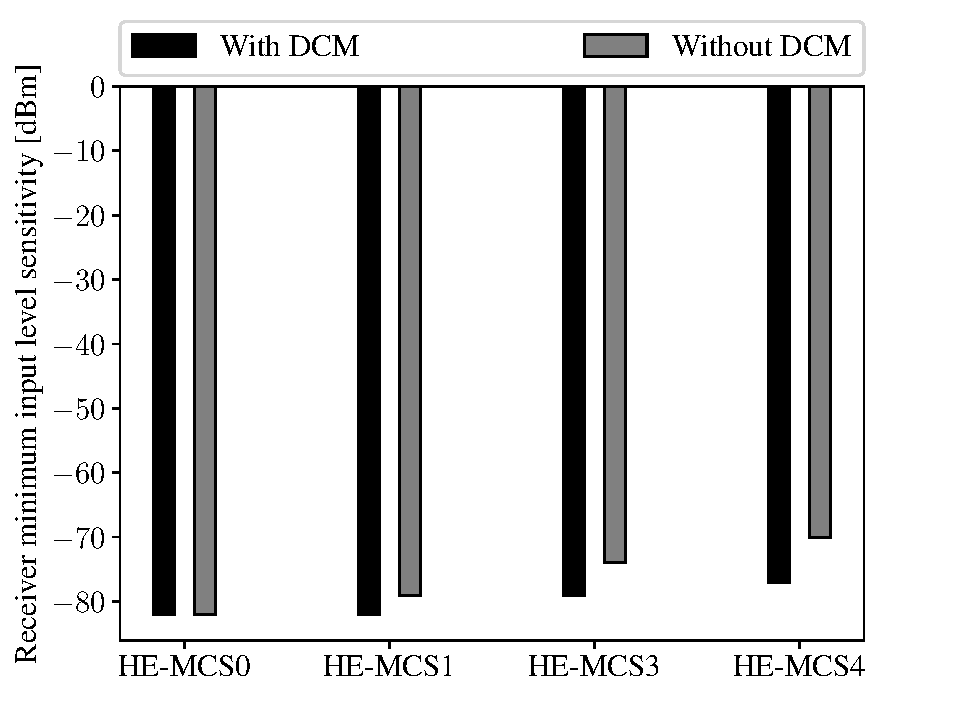
\includegraphics[width=0.75\textwidth]{figures/Receiver_minimum_DCM}
	\caption{Receiver minimum input level sensitivity for different HE-MCS values according to \cite{noauthor_ieee_2021}, where \ac{PER} is less than \SI{10}{\percent}}%
	\label{fig:ReceiverSensitivityDCM}%
\end{figure}

A similar development of the receiver minimum input sensitivity can also be observed for higher \ac{BW}, except
that the lowest value increases with \ac{BW}.

The higher probability of achieving data is reached at the expense of the data rate.
The same amount of data now takes twice as long to transmit.

\cite{noauthor_ieee_2021} lists the theoretically possible data rates.
These reveal that the maximum achievable data rate with DCM is only half of the attainable data rate without DCM.

Support for \ac{DCM} is only optional in the IEEE 802.11ax standard and can only be used for HE-\ac{MCS}-\num{0},
HE-\ac{MCS}-\num{1}, HE-\ac{MCS}-\num{3} and HE-\ac{MCS}-\num{4} for \numrange{1}{2} spatial
transmission streams \cite{noauthor_ieee_2021}.

\textcite{jacob_system-level_2020} and \textcite{triwinarko_phy_2021} mention plans,
to allow using \ac{DCM} in the physical layer of IEEE 802.11bd.

\begin{comment}
	Allowed relative constellation error versus constellation size RMS error over subcarriers and Frequency
	
	Table 27-51—Receiver minimum input level sensitivity
	
	Table 27-52—Minimum required adjacent and nonadjacent channel rejection levels
	optional feature \cite{noauthor_ieee_2021}
	
	\ac{HE} \ac{SU} \ac{PPDU} \ac{HE} \ac{ER} \ac{SU} \ac{PPDU} not for GI 800 ns \cite{noauthor_ieee_2021}
\end{comment}

\subsubsection*{\acf{ER}}
Since IEEE 802.11ax, the \ac{ER} Mode exists, which defines the new \ac{HE} \ac{ER} \ac{SU} \ac{PPDU} as physical layer amendment
\cite{noauthor_ieee_2021,afaqui_ieee_2017} .
\textcite{deng_ieee_2017} explains that the \ac{HE} \ac{ER} \ac{SU} \ac{PPDU} format is intended to extend the range of
a single station to access point transmission.
According to the authors, this is accomplished by the \ac{PPDU} containing a repetition of the HE-SIG-A field.

In addition, the authors explain that the preamble transmission power is boosted
to guarantee reliable transmission for longer ranges.
The power-boost is limited to additional \SI{3}{\decibel}
in \cite{noauthor_ieee_2021,jacob_system-level_2020}.

The IEEE 802.11ax \cite{noauthor_ieee_2021} standard defines that the \ac{HE} \ac{ER} \ac{SU} \ac{PPDU} format may only be used
when 20 Mhz transmissions with either 242-Resource Unit with HE-MCS-0 - HE-MCS-2 or 106-Resource Unit with HE-MCS-0 are used on a spatial stream.
In addition, one can use \ac{DCM}.
\textcite{sauter_wireless_2022} defines the Resource Unit as fragments of a Wi-Fi channel. The number before the Resource Unit
indicates the number of subcarriers which are part of the Resource Unit.

Optionally, the \ac{HE} \ac{ER} \ac{SU} \ac{PPDU} may also be transmitted with a \ac{GI} of \SI{800}{\nano\second},
where an additional application of \ac{DCM} is forbidden.

\textcite{jacob_system-level_2020} and \textcite{triwinarko_phy_2021} add that it is planned to use
the \ac{ER} mode also in the IEEE 802.11bd standard.

\subsubsection*{\acf{MIMO}}
In order to further exploit the physical layer capabilities, the single transmitting and receiving antenna systems called Single-Input-Single-Output can be extended to \ac{MIMO} - systems.
\textcite{sauter_wireless_2022} describe the idea behind \ac{MIMO} as the usage of multiple transmit antennas and multiple receiving antennas. Spatial multiplexing is used so that the transmitted signals
from each antenna are reflected differently on objects and can thus be received from different directions at the receiver antennas.

The authors explain that since IEEE 802.11n, it is possible to use up to \num{4} MIMO streams.
This number was increased again to up to \num{8} MIMO streams in IEEE 802.11ax \cite{noauthor_ieee_2021}.
Since data can be sent simultaneously via each MIMO stream,
the theoretical data rate can thus increase proportionally depending on the usable streams.
The mechanism is called \ac{SU}-\ac{MIMO} \cite{noauthor_ieee_2021}.

\textcite{sauter_wireless_2022} mentions that since IEEE 802.11ac it is possible to use Downlink \ac{MU}-\ac{MIMO},
which allows an \ac{AP} to transmit data to multiple \ac{STA} via different available \ac{MIMO} streams simultaneously.
According to the authors, \ac{MU}-\ac{MIMO} can increase the network throughput.
IEEE 802.11ax introduced \ac{MU}-\ac{MIMO} in the Uplink direction \cite{noauthor_ieee_2021}, where multiple \ac{STA} can transmit data simultaneously to the \ac{AP} via different available \ac{MIMO} streams.
MU-\ac{MIMO} DCM can also be applied in IEEE 802.11ax \cite{noauthor_ieee_2021}.

Another \ac{MIMO} technique is \ac{OFDMA}, which can be utilized since IEEE 802.11ax \cite{noauthor_ieee_2021, avallone_will_2021, omar_survey_2016}.
\textcite{avallone_will_2021} explains that \ac{OFDMA} enables an \ac{AP} to transmit data to multiple \ac{STA} simultaneously by dividing the available bandwidth into \ac{RU} and assigning each \ac{RU} to a \ac{STA}.
The authors add that \ac{OFDMA} can be used in both the uplink and downlink direction.
The \ac{AP} can choose the best suited \ac{RU} for each \ac{STA} and thus increase the Signal-to-Interference-plus-Noise Ratio \cite{khorov_tutorial_2019}
\textcite{behara_performance_2022} adds that \ac{OFDMA} is designed to improve the per-user throughput in high-density networks, e.q.
stadiums, airports or public transportation systems.

\subsubsection*{\acf{STBC}}
\textcite{abbas_efficient_2016} further explains that \ac{MIMO} spatial streams can be utilized to enhance the
quality of the received signal.
The Technology is called \ac{STBC}.
\textcite{santumon_space-time_2012} explains as follows.
\ac{STBC} is a technique used in Wi-Fi networks to improve the reliability and robustness of wireless communications.
\ac{STBC} encodes multiple redundant copies of data at the transmit side, which are transmitted in different spatial streams to
reduce fading and interference effects.
At the receiver side, these multiple copies are combined using a maximum likelihood detector
to retain a high-quality signal and decrease the \ac{PER}.


Here, \textcite{stamoulis_impact_2003} has investigated the potential effect of \ac{STBC} on Wi-Fi.
Their simulations showed that \ac{STBC} increase the range and robustness for IEEE 802.11a.
In addition, the authors concluded that \ac{STBC} increases the \ac{SNR} in nearly all cases at the same throughput or
even allows higher \ac{MCS} values to be used,
thus allowing a higher throughput at the same \ac{SNR}.
This results in \ac{STBC} improving the reliability and robustness of wireless communications.

\textcite{ghosh_error_2014} analyzed the error rate performance for an increased number of used antennae and found
that a lower bit error rate can be achieved
when increasing the number of transmit antennas with \ac{STBC}.

\textcite{gast_80211n_2012} and \textcite{sauter_wireless_2022} mention that \ac{STBC} can extend the signal range
due to the increased robustness.


IEEE 802.11ax stations can optionally use \ac{STBC} the following conditions \cite{noauthor_ieee_2021}:
\begin{itemize}
	\item DCM is not applied
	\item The number of spatial streams is \num{2}
	\item The \ac{GI} is not \SI{0.8}{\nano\second} and the symbol length is not \SI{12.8}{\micro\second}
\end{itemize}

\textcite{gast_80211n_2012} states that \ac{STBC} is only supported in \nicefrac{1}{5} of the Wi-Fi-certified devices.



\begin{comment}
In addition to the physical layer parameters already discussed, other technologies can be applied. IEEE 802.11ax
Beamforming
OFDMA
Group addressed frames
HE Capabilities nur so gut, wie das schlechteste Glied
\end{comment}


\subsection*{Wi-Fi Data Link Layer}

The next layer in the OSI model is the Data Link Layer.
The Data Link Layer consists of MAC and LLC functionalities.


According to \textcite[207]{kauffels_wireless_2002}, the MAC functionalities cover network entry, authentication, and media access methods.
The author explains that every \ac{AP} send beacon frames periodically to synchronise its stations in the \ac{BSS} and that the beacon frame contains the \ac{SSID}, which identifies the \ac{BSS} or \ac{ESS} of the station.
\textcite[275-276]{sauter_wireless_2022} adds that a beacon frame contains a \SI{16}{\bit} - long capability information element. Each bit here signals that the \ac{AP} provides a particular function or has a specific feature.

\textcite[220,221]{kauffels_wireless_2002} explains the following station's network entry procedure.
A station can use the passive or the active scanning mode.
The station listens for a beacon frame in the various transmission channels in passive scanning mode.
Alternatively, a station can send a probe frame in active scanning mode.
The probe frame can either contain an already known \ac{SSID} to test the presence of the \ac{AP} or include a broadcast SSID that causes all nearby \ac{AP}s to respond.
The response of an \ac{AP} to the probe frame is the probe-response frame, which contains the same information as a beacon frame.
With the information from the beacon frame, a station can start the authentication process.

For this process, \textcite[221,222]{kauffels_wireless_2002} names the two methods Open System Authentication and Shared Key Authentication.
\textcite[277]{sauter_wireless_2022} explains that Open System Authentication is based on a device making an authentication
request to the \ac{AP}.
If the \ac{AP} answers with a positive status in the Authentication Frame,
the station is included in the \ac{BSS}.
The actual encryption and authentication are then performed by the \ac{WPA} functions.
The author points out that Shared Key Authentication is no longer used today.
\textcite[122]{sommer_vehicular_2014} adds that the authentication process differs for the Ad-Hoc mode, where every station can
authenticate new stations.

After the authentication process, the station receives a time-synchronisation function with a timestamp, the physical layer
parameter configuration and the \ac{SSID} of the \ac{BSS} or \ac{ESS} \cite[220]{kauffels_wireless_2002}.
The \ac{STA} can start the media access method now.

The IEEE 802.11 standard describes the two media access methods \ac{DCF} and \ac{PCF}.

\textcite[283]{sauter_wireless_2022} explains that \ac{DCF} is based on the media access method \ac{CSMACA}.
In \ac{CSMACA}, a device willing to transmit senses in the air transmission medium for a transmitting activity.
If no other device is transmitting, the device can transmit.
In transmitting activity, the terminal must wait at least until the transmission and the \ac{IFS} are over.
Various access priorities are implemented by different \ac{IFS} lengths \cite[120]{sommer_vehicular_2014}.

Since data transmission via the air transmission medium is very vulnerable to errors,
the standard IEEE 802.11 requires that each received unicast packet be confirmed with an \ac{ACK} frame \cite[120]{sommer_vehicular_2014}.

\textcite[284]{sauter_wireless_2022} explains \ac{DCF} \ac{IFS} as the time after a transmission, which ensures that an \ac{ACK} frame can be sent before another station uses the same channel to send a data frame.
If the channel is busy, the station waits until the channel is free again.
\textcite[284-285]{sauter_wireless_2022} describes this backoff procedure as follows: each ready-to-transmit device determines
a random backoff time from a time interval called the contention window.
The device with the shortest backoff time transmits next, and all other ready-to-transmit devices restart the media access procedure to avoid multiple devices transmitting simultaneously after \ac{DIFS}.
If two devices start sending next because they randomly chose the shortest backoff time,
the transmitted signal will interfere, and the packets will not be answered with an \ac{ACK} frame.
The author adds that in case of such a faulty transmission, the contention window increases exponentially until the maximum value of retries is reached and
the contention window size is reset to the starting value.

To share the knowledge of a transmission time and the subsequently \ac{IFS}, a packet contains a \ac{NAV} that
specifies when the air transmission medium is used \cite[284]{sauter_wireless_2022}.
Collisions can occur as the \ac{NAV} information can be reset by other transmissions from a different, overlapping network.
To avoid this, IEEE 802.11ax maintains two \ac{NAV}s, one for intra-\ac{BSS} and one for inter-\ac{BSS} transmissions \cite{ieee_standard_2021ax}

The extension IEEE 802.11e introduced a amendment of \ac{CSMACA} called \ac{EDCA} \cite[121]{sommer_vehicular_2014} \cite{wu_ieee_2006}.
According to \textcite[121]{sommer_vehicular_2014}, \ac{EDCA} provides a Quality-of-Service transmission procedure,
which classifies \num{4} access categories.
The authors state that each access category has different minimum and maximum contention window sizes and different \ac{IFS} lengths, named
arbitration \ac{IFS}.

\textcite{wu_ieee_2006} explains that each access category keeps its own backoff counter and frame queue.
According to the authors, every access category is handled as an independent virtual station which tries to access the medium.
When two transmissions of different access categories collide, and both contention windows are set to zero simultaneously,
the \ac{EDCA} mechanism ensures that the access category with the higher priority wins.

The four access categories are listed in \autoref{tab:access_categories}.
\begin{table}[H]
   \centering
   \begin{tabular}{>{\raggedright}p{2.5cm}p{3.2cm}}
      \toprule
      Access Category & Priority (1 = Highest)\\
      \midrule
      Voice & 1 \\
      Video & 2 \\
      Best Effort & 3 \\
      Background & 4 \\
      \bottomrule
   \end{tabular}
   \caption{Access Categories and their priorities for IEEE 802.11e \ac{EDCA} \cite{wu_ieee_2006}}
   \label{tab:access_categories}
\end{table}

\ac{EDCA} is integrated into the modern IEEE 802.11 standard data link layer of IEEE 802.11ac \cite{ieee_standard_2020}
and IEEE 802.11ax \cite{ieee_standard_2021ax}.

In various network architectures, the "hidden station"-problem may occur.
As you can see in \autoref{fig:hidden_station}, Station A cannot sense a transmission of station B and vice versa.
In case of simultaneous transmission of both stations, interferences around the \ac{AP} may occur.
\begin{figure}[H]%
   \centering
   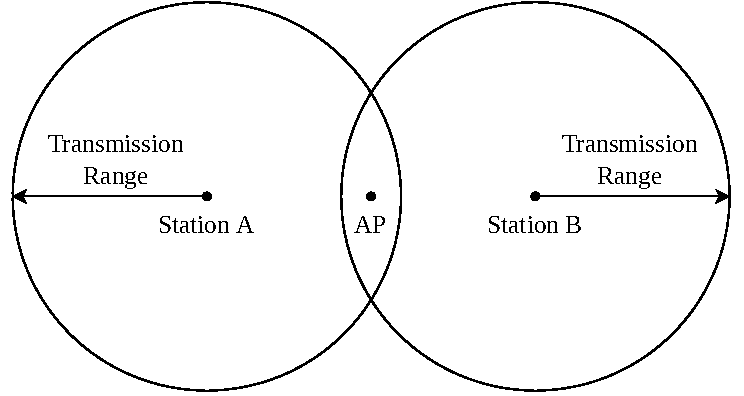
\includegraphics[width=0.75\textwidth]{Latex/figures/hidden_station.pdf}
   \caption{Hidden Station Problem, where interferences at the \acf{AP} can occur, when \acf{STA} A and B send simultaneously}%
   \label{fig:hidden_station}%
\end{figure}

To prevent the hidden station problem, \textcite[282-283]{sauter_wireless_2022} explains how a \ac{STA} can access the medium
via the \ac{RTS}/\ac{CTS} mechanism.
The \ac{STA} sends a \ac{RTS} frame to the \ac{AP} and waits for a \ac{CTS} frame.
After receiving the \ac{CTS} frame, the \ac{STA} has reserved the medium for a specific time and can send its data frame.
The successful transmission of the data frame is confirmed with an \ac{ACK} frame.
To avoid another \ac{STA} accessing the medium during the \ac{RTS} and \ac{CTS} frames, the \ac{PCF} \ac{IFS} is
shorter than the \ac{DCF} \ac{IFS}.
This mechanism allows the \ac{AP} to send the \ac{CTS} frame before another \ac{STA} can access the medium.

But the author states that the \ac{RTS}/\ac{CTS} mechanism is usually not configured because it introduces additional
overhead of the \ac{RTS} and \ac{CTS} frames, which is only worth it when the data frame is large.

Larger frames can also be split into smaller frames to reduce the probability of collisions.
This procedure, called fragmentation, divides the data into up to \num{16} frames
when a specific data length threshold is exceeded \cite{ieee_standard_2009n}.
The fragmented frames are transmitted by the three following different \ac{ACK} policies in \autoref{fig:ACKS}, which are described by \textcite[334-335]{sauter_wireless_2022}.

\begin{figure}%
    \centering
    \subfloat[normal ACK]{\label{fig:ACK}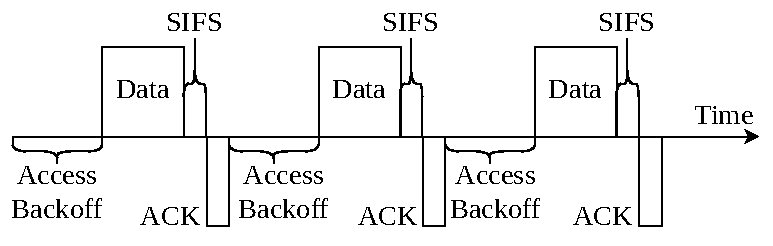
\includegraphics[width=0.7\textwidth]{Latex/figures/normalACKs}}%
    \\
    \subfloat[fragmentation]{\label{fig:Fragmentation}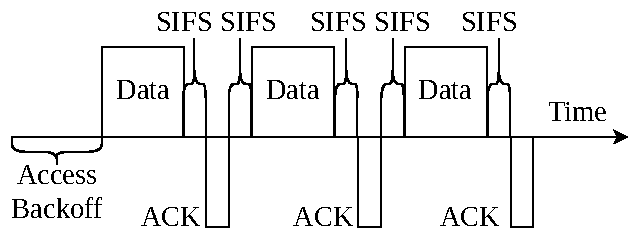
\includegraphics[width=0.7\textwidth]{Latex/figures/fragmentation}}%
    \\
    \subfloat[fragmentation and Block ACK]{\label{fig:BLOCKACK}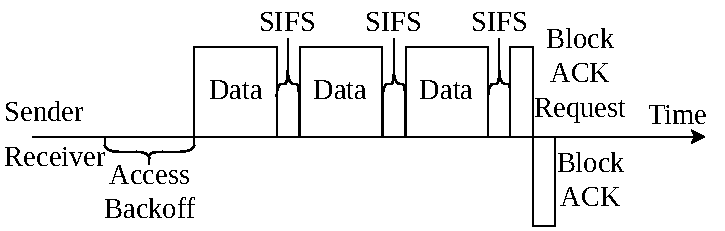
\includegraphics[width=0.7\textwidth]{Latex/figures/BlockACK}}
    \caption{Data transmission between a sender and receiver in regards to the time with normal \acf{ACK} \autoref{fig:ACK},
    fragmentation \autoref{fig:Fragmentation} and additional Block \acs{ACK} \autoref{fig:BLOCKACK}}%
    \label{fig:ACKS}%
\end{figure}

Using the standard \ac{ACK} policy, the sender applies the \ac{DCF} mechanism before sending each frame.
After each transmission, the sender also waits
for an \ac{ACK} frame from the receiver.

Instead of operating in the \ac{DCF} mode, the sender
can also send the next frame after waiting for the \ac{SIFS} time when the \ac{ACK} frame has been received.
This is displayed in \autoref{fig:Fragmentation} and saves the overhead of acquiring the medium again.

Additional transmission time can be saved using the Block \ac{ACK} policy, shown in \autoref{fig:BLOCKACK}.
The sender sends the first frame and waits for the \ac{ACK} frame.
After transmitting all fragments, the sender sends the Block \ac{ACK} request.
The receiver sends the Block \ac{ACK} frame, which contains the information of all received frames.
All missing frames are retransmitted.
The Block \ac{ACK} frame can be sent delayed when some processing time is required.

The IEEE 802.11 standard defines how every Block \ac{ACK} session is started and ended \cite{ieee_standard_2009n, ieee_standard_2021ax}.
Every Block \ac{ACK} session is started with an add Block Acknowledgment (ADDBA) request frame, which the sender sends and
contains the session parameters.
The receiver sends an \ac{ACK} and answers with an add Block Acknowledgment (ADDBA) response frame.
After the sender acknowledges the response frame, the Block \ac{ACK} session is established.
The Block \ac{ACK} session is ended with a delete Block Acknowledgment (DELBA) frame, which is sent by the sender and acknowledged by the receiver.

The Block \ac{ACK} policy can be used in IEEE 802.11n \cite{ieee_standard_2009n}, IEEE 802.11ac \cite{ieee_standard_2020} and IEEE 802.11ax \cite{ieee_standard_2021ax}.
In the IEEE 802.11p standard, the Block \ac{ACK} policy can be added as an optional feature \cite{ieee_standard_2010p}.





\begin{comment}
	CF Parameter set-element


MAC Header


    \cite{khorov_tutorial_2019}
Power Management Modes
Enhanced Time TWT Enhanced Microsleep

Spatial Reuse
Adaptive Power and Sensitivity Thresholds, BSS COlor

Quiet Period

Midamble Preamble


more levels of fragmentation

\end{comment}






%\subsection{IEEE 802.11ac - Wi-Fi 5}
The 5th generation WLAN is \ac{ac} and operates in the \SI{5}{\giga\hertz}  frequency range \cite{dhawankar_throughput_2018}.

According to \textcite{perahia_gigabit_2011}, \ac{ac} is a further evolution of IEEE 802.11n, where \ac{ac} adds to the known bandwidth of \text{IEEE 802.11n} of \SI{40}{\mega\hertz} the bandwidths \SI{80}{\mega\hertz},\SI{160}{\mega\hertz} and the interrupted bandwidth of \SI{80}{\mega\hertz} + \SI{80}{\mega\hertz}.

nach \textcite{sauter_wireless_2022} ist die Aufspaltung in zwei 80 Mhz Kanäle sehr nützlich, wenn das frequenzband reservierte Regionen enthält. Dadurch kann ein 160 Mhz breiter Kanal um  eine reservierte region des frequenzbandes gebaut werden.

The modulation technique used is \ac{OFDM}.
Additionally, a new \ac{MIMO} Downlink functionality for multiple users, called DL MU-MIMO, with up to 8 partial streams is introduced according to the authors. Together with the new \ac{MCS} from 64 \ac{QAM} to 256 \ac{QAM}, these three enhancements ensure that a higher data rate can be achieved. The maximum data rate is \SI{6.9}{\giga\hertz} according to the authors.

As declared by \textcite{abdelrahman_comparison_2015}, the 5th generation of WLAN has made it possible to expect better performance as in addition to a longer communication range compared to the previous IEEE 802.11 standards This statement could be proven at least for indoor range.  \textcite{dhawankar_throughput_2018} were able to demonstrate that \ac{ac} with a range of over \SI{60}{\metre} enables a longer indoor communication range than previous IEEE 802.11 standards.


new Physical Layer Very High Throughput (VHT) Physical Layer

80 Mhz

Beamforming 

\subsection{IEEE 802.11ax - Wi-Fi 6}

The 6th generation of WLAN is \ac{ax}. \textcite{khorov_tutorial_2019} reveals what has changed from \ac{ac} to \ac{ax}. For this, the authors make the following statements.

\ac{ax} uses the same bandwidths in the \SI{5}{\giga\hertz} range and can also operate in the \SI{2.4}{\giga\hertz} frequency range with a maximum bandwidth of \SI{40}{\mega\hertz}. Similar to DL MU transmission, \ac{ax} enables UL MU transmissions. These can also use \ac{OFDMA} in addition to the already known \ac{MIMO} of \ac{ac}. \ac{OFDMA} groups the orthogonal frequency subcarriers into \ac{RU}s, which can be selected by the transmitter for optimal transmission to the receiver. This increases the \ac{SINR}.

An extension in the PHY layer are the new \ac{MCS}'s of up to 1024-\ac{QAM}. However, these should only be used with very good channel characteristics.
 For better outdoor communication \ac{ax} increases the \ac{OFDM} symbol duration from \SI{3.2}{\micro\second} for \ac{ac} to up to \SI{12.8}{\micro\second} and the \ac{OFDM} Guard Interval from a maximum of \SI{0.8}{\micro\second} for \ac{ac} to up to \SI{3.2}{\micro\second}.   
 
MIMO und OFDMA MU Streams

BSS Coloring

Backward Kompatibilität über CTS Reservierungen.

Tabelle Vergleich

\begin{table}
	\centering
	\begin{tabular}{>{\raggedright}p{1.7cm}p{5.4cm}p{3.4cm}}
		\toprule
		Parameter & IEEE 802.11ac & IEEE 802.11ax \\
		\midrule
		Frequency bands & \SI{5}{\giga\hertz}&
		\SI{2.4}{\giga\hertz}, \SI{5}{\giga\hertz}, \SI{6}{\giga\hertz}\\
		Symbol Length & \SI{3.2}{\micro\second}&
		\SI{12.8}{\micro\second}\\
		\ac{OFDM} Subcarrier Spacing &
		\SI{312.5}{\kilo\hertz} &
		\SI{78.125}{\kilo\hertz} \\
		\ac{OFDM} Subcarriers in \SI{80}{\mega\hertz} &
		256 &
		1024 \\
		max. \ac{MCS} &
		256 -\ac{QAM} &
		1024 -\ac{QAM} \\
		max. \ac{GI} &
		\SI{0.8}{\micro\second} &
		\SI{3.2}{\micro\second} \\
		\bottomrule
	\end{tabular}
	\caption{Comparison of IEEE 802.11ac and IEEE 802.11ax}
	\label{tab:SensorNetworkApplications}
\end{table}

\begin{comment}
	\section{Modell für drahtlose Übertragungssysteme}
Abb 2.3.1  Modell einen Übertragungssystems
Beschränkungen und Regelungen Frequenzwahl, Sendeleistung
Analoger Kanal Störungen: thermisches Rauschen, Nebensprechen, Impulsstörungen
\fi

\end{comment}

\section{Related Work}
Since my undergraduate thesis \footnote{https://github.com/klautenschlaeger/mvsc Accessed: 5.2.2023} about "Wirelessly Networked Coordination of Automatic Section Control for Agricultural Machines"
, I have been working on the topic of wireless infield communication (WIC). I conducted both field experiments and
simulations to investigate the performance of LoRa as a technology to exchange process data in
meshed Automatic Section Control, a prototypical application of connected vehicles in the agricultural domain.
A summary of my results is published in a paper \cite{lautenschlaeger_beyond_2022}.
In my undergraduate thesis and paper, I described the current state of research in the field of WIC.

The first research paper on WIC that I found was from \textcite{ali_multi-agent_2010}. The authors
developed a system based on General Packet Radio Service (GPRS) to exchange position data between \ac{TM}s and combine
harvesters to guide empty \ac{TM}s to a combine harvester.

\textcite{smolnik_5g_2020} describes the research project "5G Netmobil" in which the authors investigated how existing technologies like
IEEE 802.11 or 3GPP LTE can be integrated into 5G technologies to enable Agricultural Platooning Services. The research plan was to evaluate the use of \ac{UDP} and Basic Transport Protocol (BTP) to exchange guidance data via
the underlying technologies 3GPP LTE and 5G V2X and IEEE 802.11p. The authors implemented a system using 802.11p,
as according to their technical analysis, this technology already fulfils the requirements for data rate, latency
and the number of participants. The authors report that the project results demonstrated that achieved
latencies were five times lower than the defined maximum latency of \SI{50}{\milli\second} for Agricultural Platooning Services.

Further research on \ac{WIC} is not based on cellular networks. \cite{zhang_method_2009} used IEEE 802.15.4 to implement a
prototype of an Agricultural Platooning Service, where the developed system exchanges relevant control data between a leading tractor
to guide a following tractor.

\textcite{smolnik_5g_2020} states, that the developed system of \textcite{zhang_method_2009} is part
of the project \textit{Elektronische Deichsel für landwirtschaftliche Arbeitsmaschinen (EDA)}
and it was further improved within the scope of project \textit{Elektronische Deichsel für landwirtschaftliche Arbeitsmaschinen mit Umfeldsensorik und zusätzlichen Geoinformationen (EDAUG)}.


\textcite{klingler_agriculture_2018} investigated how IEEE 802.11p can be used for \ac{WIC}. Experiments revealed
that data could be exchanged over a maximum range of 1700 m, where \ac{LoS} was lost. But during the
measurement in an agricultural work scenario from the corn harvest, there were collapses in the \ac{RSS}
due to shadowing effects of the machines. The authors point out that the size and shape of the forage harvester
can cause intensified shadowing effects.

As of July 2, 2021, the frequency spectrum of IEEE 802.11p in the United States of America, ranging from
\SIrange{5,850}{5,925}{\giga\hertz}, has been split. The upper \SI{30}{\mega\hertz} are reserved for
Intelligent transportation systems now. The lower \SI{45}{\mega\hertz} have been released for unlicensed
operations \cite{noauthor_use_2021}.

Since the use of IEEE 802.11p has now been newly
regulated by the FCC, the \ac{WIC} project group is looking for an alternative technology that enables \ac{WIC}.

There are also more developments in the industry field of \ac{WIC}. In this context, \textcite{thomasson_review_2018} describe the John Deere Machine Sync and Case IH V2V systems as follows:

John Deere Machine Sync enables the \ac{WIC} use cases Process Data Exchange and Agricultural Platooning Service. \textcite{liu_automation_2022} have extended the system to use Combine Harvesters, adding that the Machine Sync system is based on \textcite{metzler_system_2006}'s patent.
\textcite{smolnik_5g_2020} adds that John Deere Machine Sync is only available for a subgroup of John Deere machine types and cannot be used with machines of other brands.

Case IH V2V also offers an agricultural platooning service. However, according to the authors, the system can only be used for harvesting and loading scenarios.

Also currently on the market is the Raven Autonomy™ Driver Assist Harvest Solution \footnote{https://ravenind.com/products/autonomy/driver-assist-harvest-solution Accessed: 5.2.2023} system from Raven Industries. This system allows the harvester to take control of a \ac{TM} from a distance of \SI{70}{\metre}. The harvester then automatically guides the \ac{TM} into the perfect position to load the harvested crop onto the \ac{TM} via the spout. Once the harvesting and loading process is complete, the driver of the \ac{TM} driver retakes control.

A comparable system is CartACE from AgLeader \footnote{https://www.agleader.com/harvest/cartace/ Accessed: 5.2.2023}

The technology used in the mentioned systems is not known. In response to questions about how the systems can be used on farms worldwide and what prerequisites must be created for this, the manufacturers refer to the regional distribution options.


\todo{Paul outdoor performance, table selbst done}

Wireless communication technologies are also used to implement wireless sensor networks in the agricultural domain.

According to \textcite{ahmed_internet_2018}, wireless sensor networks in the agricultural domain can be used to monitor soil and water conditions, plant diseases and farm automation solution
or track animals or assets. The authors mention similar requirements for wireless sensor network applications  compared to \ac{WIC} applications.
For example, asset tracking applications require a low latency and must support asset mobility.
The results of the authors indicate, that fog computing can lessen the latency and the required bandwidth compared to cloud computing.
When a higher data rate is required, the authors recommend to wi-fi technologies like IEEE 802.11n or IEEE 802.11ac.

As wireless sensor networks for agricultural applications, they must be able to operate in the same agricultural environment as \ac{WIC} applications.
\textcite{brinkhoff_characterization_2017} describe as requirements, that they expect a limited cellular network coverage and complex outdoor
environments with large water areas, different crop vegetations and other obstacles or various weather conditions. The
reseachers developed a wirless sensor network based on IEEE 802.11b, where they exchanged data between an \ac{AP} and multiple stations on
a cotton and rice field. The authors report, that they easily a achieved communication of \SI{1000}{\metre} in a \ac{LoS} scenario.
They mention, that different wheater conditions have little impact on the communication reliability. A big influence on the communication range is
the height above ground or the crop vegetation, where the authors recommend to use at least a height of \SI{0.2}{\metre}.

Aust:

paul:


\section{Harvest and Loading Processes as a Use Cases for \ac{WIC}}
The Forage harvester has proven to be an essential agricultural machine for harvest
ing and loading forage. \textcite{seifert_feldhacksler_1962} define a forage harvester
as an agricultural loading machine for nearly all types of animal feed. According to the authors, a  forage harvester can load the following animal feed by mounting different cutting and loading devices: Hey, Straw, Corn, Grass and Clover.
\begin{figure}%
	\centering
	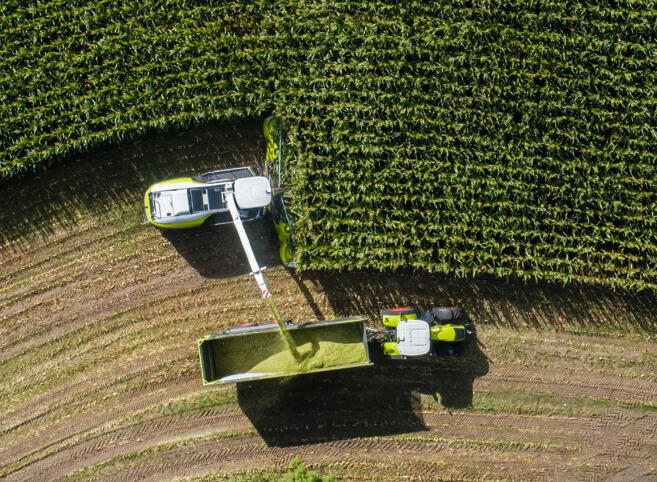
\includegraphics[width=0.6\textwidth]{figures/claas_harvest_side.png}
	\caption{\ac{FH} and \ac{TM} while }%
	\label{fig:normal}%
\end{figure}

In the harvesting and loading process, a \ac{TM} typically drives alongside or behind the \ac{FH} so that the \ac{FH} can load the harvested goods onto the trailer of the \ac{TM} using the spout. Drivers operate both machines and try to keep the speed and distance so that the spout only throws the harvested goods into the trailer of the TM. An image of a corn harvesting and loading process can be seen in \autoref{fig:normal}.

Taking a corn harvest scenario as an example, I looked up key figures in \cite{faustzahlen2018}, a standard reference book in agricultural literature. This book contains key figures of agricultural processes, which 80 experts have compiled. The key figures, which are shown in \autoref{tab:DataSilageHarvest}, are dependent on the \ac{PPD} and show the large amount of forage harvested by a  \ac{FH} every hour.
\begin{table}[H]
	\centering
	\begin{tabular}{>{\raggedright}p{4.9cm}p{1.8cm}p{1.8cm}p{1.8cm}}
		\toprule
  		\ac{PPD} &  \SI{20}{\tonne\per\hectare} & \SI{30}{\tonne\per\hectare} & \SI{50}{\tonne\per\hectare}\\
		\midrule
		Required \ac{TM}s & \num{5}&
		\num{7} & \num{10} \\
		Harvested volume in \si{\cubic\metre\per\hour} &
		\num{285.7}-\num{333.3}
		& \num{428.6}-\num{500.0} &
		\num{595.7}-\num{695.0}\\
		Filled \ac{TM} loads in \si{\per\hour} &
		\num{5.7} - \num{6.7}
		& \num{8.6} - \num{10.0} &
		\num{11.9} - \num{13.9}\\
		Harvested mass in \si{\tonne\per\hour} & \num{100}
		& \num{150} &
		\num{208.5} \\
		\bottomrule
	\end{tabular}
	\caption{Key figures from \cite{faustzahlen2018} of corn harvest of a \ac{FH} with a working width of \SI{6.2}{\metre} in a \SI{80}{\hectare}-field in regards to \ac{PPD}}
	\label{tab:DataSilageHarvest}
\end{table}

The harvesting and loading processes are examples of the use of agricultural Platooning Services as described by 
\textcite{zhang_method_2009}.
This Platooning Service creates a leader and follower system where an uncrewed agricultural machine follows a leading operated agricultural machine.
The operated \ac{FH}, as a leader, sets the path and speed and transmits the data via \ac{WIC} to the \ac{TM}. Based on the path and speed data of the \ac{FH}, \ac{TM} follows unmanned with a longitudinal and lateral offset, as \autoref{fig:offset} displays.
\begin{figure}[H]
	\centering
	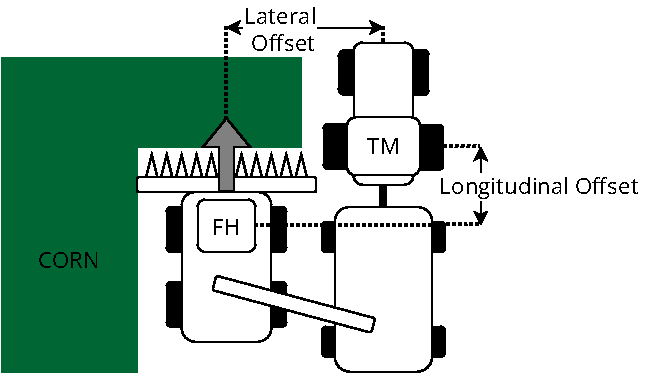
\includegraphics[width=0.65\textwidth]{figures/offset_platoon.pdf}
	\caption{Lateral and longitudinal Offset between the two agricultural machines \ac{FH} and \ac{TM} in a corn harvest scenario}%
	\label{fig:offset}%
\end{figure}

The application of platooning services offers many advantages.
The \ac{TM} is positioned optimally to the \ac{FH} so that the forage can be loaded ideally from the \ac{FH} onto the \ac{TM}.

Because, as displayed in \autoref{fig:workforce_agri}, fewer and fewer workers are working in agriculture, platooning services for harvest and loading processes can save and free up labour for other activities \cite{liu_automation_2022}. As stated in \autoref{tab:DataSilageHarvest}, already ten drivers for the \ac{TM}s are needed in the corn harvest process with a high \ac{PPD}. Using an agricultural Platooning Service, each \ac{TM} can drive unmanned in the field, leading to fewer workers needed in the corn harvest process.

\begin{figure}[H]
	\centering
	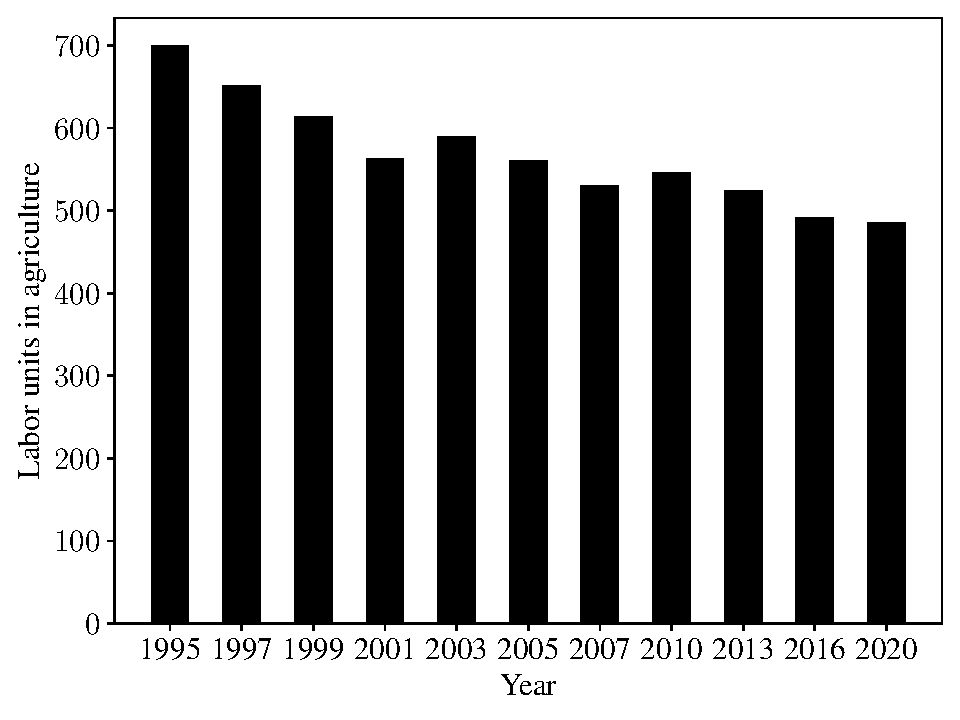
\includegraphics[width=0.75\textwidth]{figures/WorkForceAgriculture.pdf}
	\caption{Decrease in the agricultural labor force in Germany based on the data from \cite{bmel2020}}%
	\label{fig:workforce_agri}%
\end{figure}

\textcite{smolnik_5g_2020} adds that platooning services at the platoon level can reduce drivers' workload so that they can focus on optimally adjusting the machines.
In addition, \ac{TM}s can be guided to the \ac{FH}s in a targeted manner so that logistics processes in the field can be improved.

At the same time, the harvest and loading processes are examples of the video streaming \ac{WIC} use case. During these harvest and loading processes, the spout of the \ac{FH} must be controlled to set the loading position of the forage into the trailer of the \ac{TM}.

According to \textcite{murcia_quadrotor_2014}, different spout guidance and control systems have been developed to automate the filling of the trailer. Spout guidance and control systems use a camera attached to the spout to determine the fill volume at each point of the trailer via machine vision and set the spout to fill the empty parts accordingly. The author describes Autofill - systems from Claas and Intellifill - systems from CNH Industrial as examples of spout guidance systems. 

Streaming the video of a camera at the spout from the \ac{FH} to the \ac{TM} would be a practical application of the video streaming use case in the harvesting process. If the \ac{TM} driver can watch a live stream of the trailer's fill level, he will always be
informed and knows when the trailer is full and can drive the forage back to the
farm.

\chapter{Analyzing Corn Harvest Process Data}

To gain a better insight into requirements of the \ac{WIC} use cases Platooning and Streaming Services, I analysed process data of a corn harvest scenario as the example for I collected GPS tracks of  a  \ac{FH} and two to three \ac{TM}s harvesting corn on a field in Germany on two days in September. For this, I placed tablets in the driver's cabs of  a  \ac{FH} and three \ac{TM}s, which recorded the position and speed in an NMEA data stream of the tablet's GPS every second. 

% wahrscheinlich raus
The workflow for collecting the corn harvest process data was as follows. 
I handed out the tablets to the drivers, which left the farm with the tablets in the driver's cabs to drive to the field in the morning. The tablets recorded the position and speed of the \ac{FH} and the \ac{TM}s all day. During breaks, the tablets continued to capture the NMEA data stream of their GPS even if the positions and speed did not change.

After recording the process data, I anonymized it. 
First, I deleted data points of the log files until the recorded accuracy of the following data points was less than \SI{2}{\metre}. Then, I replaced the timestamp and the date for all data points with a continuous index.

To gain a better insight into requirements of the \ac{WIC} use cases Platooning and Streaming Services, I analysed process data of a corn harvest scenario as the example for I collected GPS tracks of a  \ac{FH} and two to three \ac{TM}s harvesting corn on a field in Germany on two days in September. For this, I placed tablets in the driver's cabs of a  \ac{FH} and three \ac{TM}s in the morning, which recorded the position and speed in an NMEA data stream of the tablet's GPS every time second. 

After I collected the tablets in the evening, I anonymised the recorded process data. 
Starting, I deleted data points of the log files until the recorded accuracy of the following data points was less than \SI{2}{\metre}. Then, I replaced the timestamp and the date for all data points with a continuous index.

After that, I anonymised the location data by adding a random offset to the GPS coordinates. As a result, this procedure moved the areas to a random location in the world with a continuous index as a timestamp, where the exact date is unknown.

The goal of analysing the corn harvest data was to investigate the machines moving in the working scenarios relative to each other. The machines' speed and distance in tracked harvest platoons data may result in new use case requirements, e.g. latency or communication range of Platooning and Streaming Services. The machinery movement profile can be used to identify when shadowing effects may occur in the work scenario or when machines meet in the field.

For this purpose, I built a dashboard with the Python framework \textit{Dash}\footnote{https://dash.plotly.com/introduction Accessed: 5.12.2022}. I initially plotted all the positions in a polyline for each machine
on a map in the dashboard. An added slider allows one to set a time interval that narrows down the data points for display in the dashboard. In addition, one could select which \ac{TM}s are displayed next to the \ac{FH}. For the chosen time interval, the distance and velocity difference between the selected \ac{TM}s and the \ac{FH} were plotted in graphs as time histories.

In the dashboard, I could get an overview of the machine's behaviour 
before, during, and after the overloading scenario.
The overview shows that a \ac{FH} is nearly always in the overloading process with a \ac{TM}. In doing so, the \ac{FH} may occasionally stay in the same place if the cutter is clogged or there is a transition of \ac{TM}s where a full \ac{TM} moves away from the \ac{FH} and an empty \ac{TM} catches up to the \ac{FH} to take over the forage.

A \ac{TM} is in a platoon with a  \ac{FH} if it is close to the \ac{FH} and they are moving at nearly the same speed. The distance between \ac{TM} and \ac{FH} increases during a turning manoeuvre on the field. Since both machines have different curve radii in a turning manoeuvre, a different machine's speed can be observed to finish turning simultaneously.
\textcite{smolnik_5g_2020} also describes these observations and indicates that this different speed adds a new level of complexity.

A new harvesting process begins as soon as the machines finish turning and are at the beginning of a new lane.
Again, the machines drive closely and nearly at the same speed to harvest and overload forage.

Furthermore, another \ac{TM} can sometimes be close to the \ac{FH}. This \ac{TM} is empty and waits to work with the \ac{FH} in the next platoon. For that purpose, the empty \ac{TM} drives close behind the current platoon at the same speed to not catch up even closer to the platoon and be ready in the vicinity.

Based on the above observations, I developed an intelligent algorithm for detecting platooning scenarios in the recorded harvest process data. It uses a weighted sum of distance and speed difference between \ac{FH} and \ac{TM} to detect the platooning scenarios.

For verification purposes, I displayed the found platoons scenarios on the map and confirmed the algorithm's functioning. 

Additionally, I implemented the following further verification method. 
I observed that a fully loaded \ac{TM} leaves the field via one of the field exits to bring the crop to a farm building. Via a check, if a \ac{TM} has left the field and thereby passed the exit after leaving a platoon, wrongly recognized platoons can be discarded.

\begin{figure}%
	\centering
	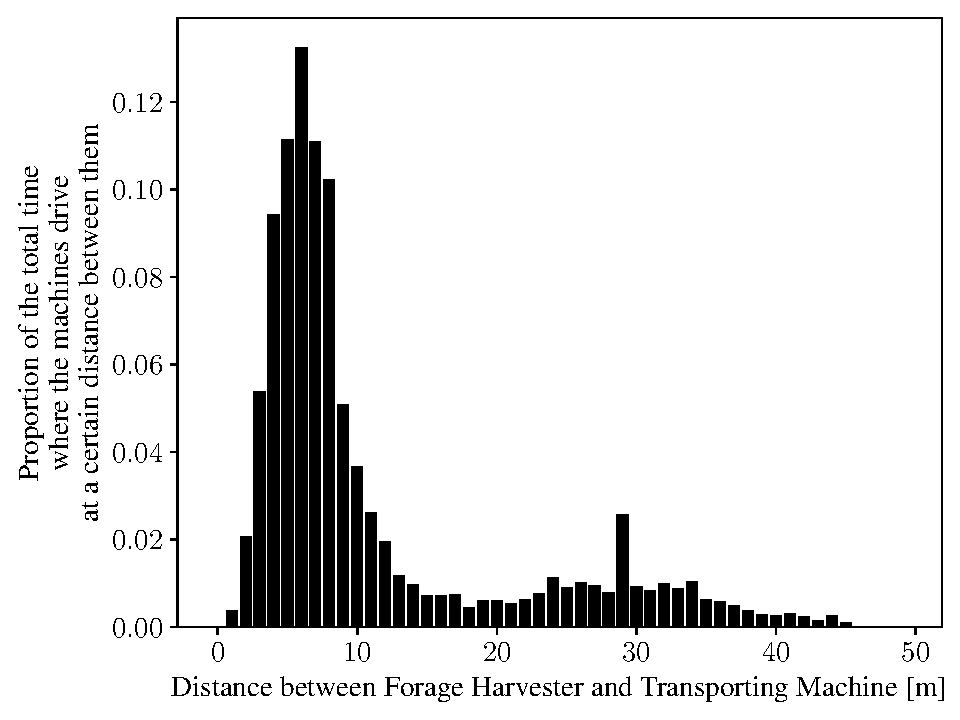
\includegraphics[width=0.85\textwidth]{figures/distanceHarvestSzenario.pdf}
	\caption{Distribution of time proportions where a given distance was between \ac{FH} and \ac{TM} in a harvest platoon scenario.}%
	\label{fig:distance}%
\end{figure}
\begin{figure}%
	\centering
	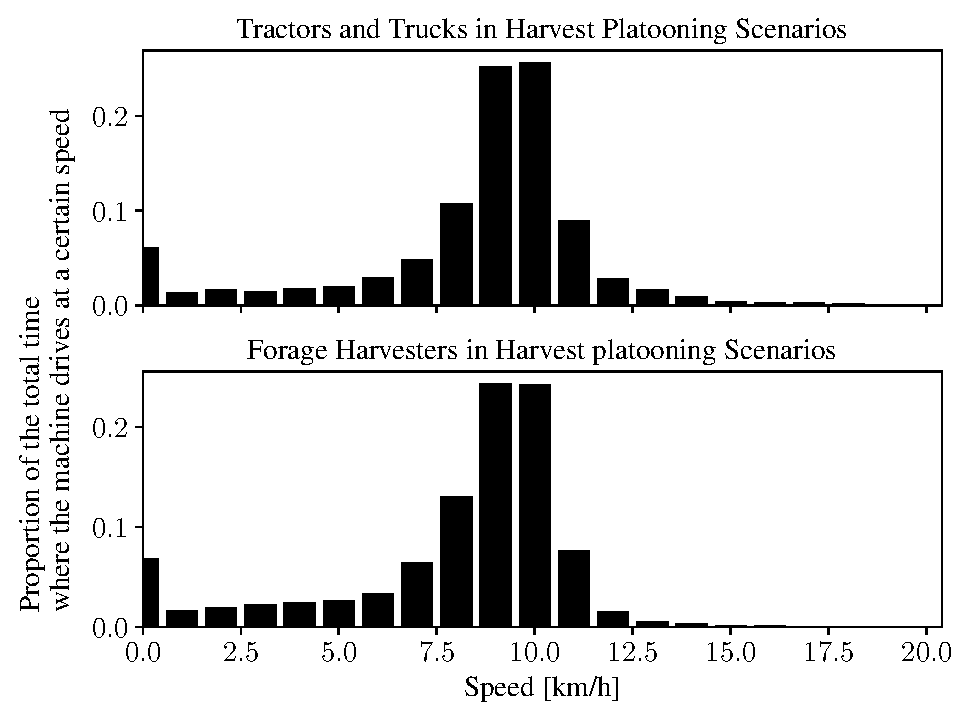
\includegraphics[width=0.85\textwidth]{figures/speedHarvestSzenario.pdf}
	\caption{Distribution of time proportions where \ac{FH} and \ac{TM} drove with a certain speed in a harvest platoon scenario}%
	\label{fig:speed}%
\end{figure}

After the platoons scenarios were correctly detected, I included the data points before each platoons scenario till a maximum distance of \SI{50}{\metre} between \ac{FH} and \ac{TM} was exceeded. These data points are also relevant to the requirements because at the beginning of an agricultural platooning service, the \ac{FH}, as the system leader, must be able to guide an empty \ac{TM} to the appropriate position for overloading.

For the detected data points of the platooning services from recorded data of the corn harvest, the proportion where the \ac{FH} and \ac{TM} move in a specific distance is shown in \autoref{fig:distance}. For the same data points, the proportion in which \ac{FH} and \ac{TM} move at a given speed is available in \autoref{fig:speed}.

These analysing results show that the \ac{TM} and the \ac{FH} usually move with a distance of less than \SI{10}{\metre}. In addition, the distance can also be higher, e.g. in turning manoeuvres or before the overloading process.

\textcite{smolnik_5g_2020} specifies the required communication range of platooning services in the corn harvest process as less than \SI{30}{\metre}.

One notable observation in \autoref{fig:speed} is that the \ac{FH} and \ac{TM}s in the corn harvesting platooning scenario often travel at a speed of approximately \SI{10}{\kilo\metre\per\hour}. This speed is significantly higher than the average speed of \SI{5.6}{\kilo\metre\per\hour} of a \ac{FH} in an entire corn harvesting process from \cite{faustzahlen2018}. It is necessary to classify that in the year of the recorded data was little precipitation, so the corn was not dense and high, and the last speed value is an average value of the entire corn harvest process, which can be calculated from the data in \cite{faustzahlen2018}.
Nevertheless, the recorded data shows that a platooning service in agriculture must also be designed for higher speeds. 

In \autoref{fig:speed} is a local maximum at a speed of \SI{0}{\kilo\metre\per\hour}. In a harvest platoon scenario, \ac{FH} and \ac{TM} can stand still briefly when the cutting device is jammed.
The driver's specific actuation usually clears the forage jam of the cutting device so that the platoon can continue its work.

\textcite{smolnik_5g_2020} defines an average speed of \SI{4.5}{\kilo\metre\per\hour} for the development of platooning services in the corn harvesting process. Depending on the \ac{PPD}, the speed can vary from \SIrange{2}{6}{\kilo\metre\per\hour} according to the authors.
The authors do not give a basis for the figures. However, the report is from the agricultural machinery manufacturer Claas, which is a major producer of \ac{FH} worldwide and thus should have expertise in the topic.

\textcite{klingler_agriculture_2018} investigated the suitability of IEEE 802.11p for \ac{WIC}. The authors detected that shadowing effects occur in the harvest scenario. The authors explain the effect because another tractor or the spout of the \ac{FH} was in \ac{LOS}.
\begin{figure}%
	\centering
	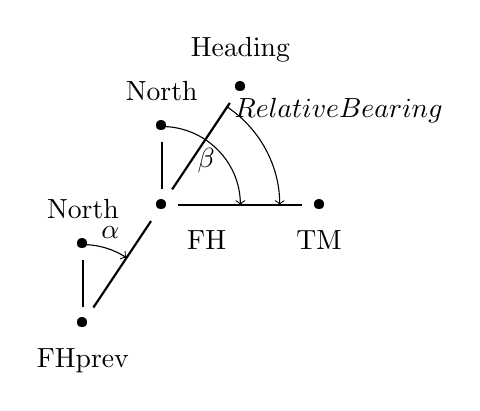
\begin{tikzpicture}
		\node[label=below right:FH](a) at (0,0) {\textbullet};
		\node[label=above:North](d) at (0,1) {\textbullet};
		\node[label=above:Heading](c) at (1,1.5) {\textbullet};
		\node[label=below:TM](b) at (2,0) {\textbullet};
		\node[label=below:FHprev](e) at (-1,-1.5) {\textbullet};
		\node[label=above:North](f) at (-1,-0.5) {\textbullet};
		\draw [thick] (a) -- (b);
		\draw [thick] (a) -- (c);
		\draw [thick] (a) -- (d);
		\draw [thick] (a) -- (e);
		\draw [thick] (e) -- (f);
		\draw 
		pic["$\beta$", draw, <-,angle eccentricity=0.8, angle radius=1.0cm]
		{angle=b--a--d}
		pic["$\alpha$", draw, <-,angle eccentricity=1.2, angle radius=1.0cm]
		{angle=a--e--f}
		pic["$Relative Bearing$", draw, <-, angle eccentricity=1.7, angle radius=1.5cm]
		{angle=b--a--c};
	\end{tikzpicture}
	\caption{Relative bearing between \ac{FH} and \ac{TM} which is calculated using the previous location of \ac{FH} by using $\beta$ and $\alpha$ for \autoref{eq:RelativeBearing}}%
	\label{fig:bearing_fh_tm}%
\end{figure}
I reviewed the recorded position data to get an overview of the \ac{TM}'s position relative to the \ac{FH}  in the overloading process. The relative bearing is the angle between B, and the heading of point A. Using the previous position of the \ac{FH}, the relative bearing between \ac{FH} and \ac{TM} can be calculated with the angles $\alpha$ and $\beta$ in \autoref{fig:bearing_fh_tm} as:
\begin{equation}\label{eq:RelativeBearing}
	Relative\_Bearing = \beta - \alpha	,
\end{equation}
Assuming that the \ac{FH} does not move backwards, the relative bearing describes the relative angle from the \ac{FH} to \ac{TM}. The result is displayed in \autoref{fig:bearing}. It can be observed that the \ac{TM} is mainly close to the \ac{FH} at an angle of \SIrange{30}{150}{\degree} at a distance between \SIrange{0}{10}{\metre}. 

\begin{figure}[H]
	\centering
	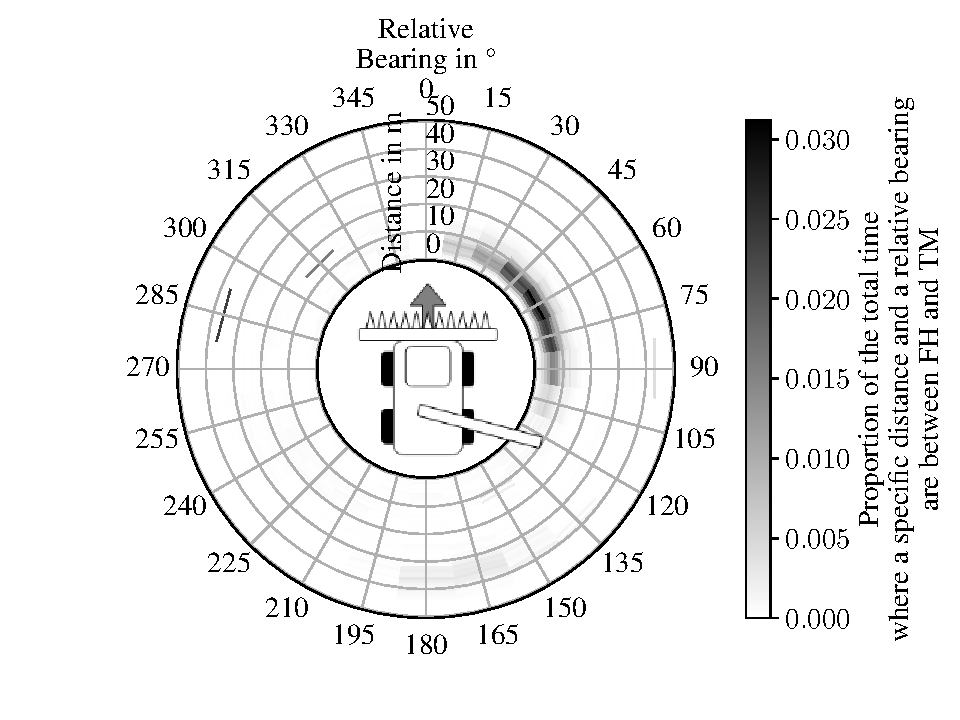
\includegraphics[width=0.99\textwidth]{figures/bearingHarvestScenario50.pdf}
	\caption{Distribution of time proportion at specific distances and relative bearings between \ac{FH} and \ac{TM}}%
	\label{fig:bearing}%
\end{figure}

In addition, it is noticeable that the machine can also be directly behind the \ac{FH}. This driving behind each other is common when a new part of the field is being cut in harvesting, as shown in \autoref{fig:startpart}. When there is a greater distance between \ac{TM} and \ac{FH}, the \ac{TM} is usually behind the FH at an angle of \SIrange{157.5}{187.5}{\degree}. At these moments, the \ac{TM} is empty and closes up to the \ac{FH} to operate in a new platooning Service together. 

\begin{figure}[H]%
	\centering
	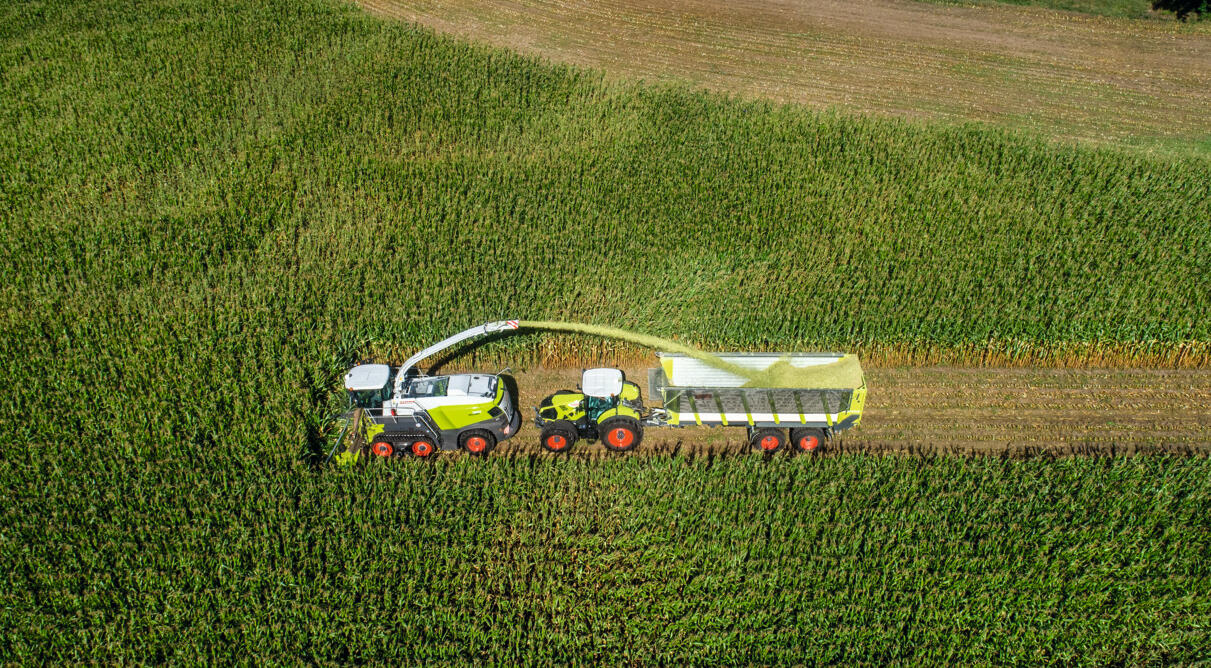
\includegraphics[width=0.8\textwidth]{figures/claas_harvest_behind.png}
	\caption{\ac{FH} and \ac{TM} start cutting a new field section}%
	\label{fig:startpart}%
\end{figure}

Another notable fact is that the \ac{TM} hardly ever stayed to the left of the \ac{FH}. Since the \ac{FH} often made left turns, the crop was usually already harvested to the right of the \ac{FH} so that the \ac{TM} could drive there without running over the crop. On rare occasions, the \ac{TM} was also to the left of the \ac{FH}. Such a platooning scenario can be an exception or a driving manoeuvrer to start cutting a new part of the field.   

The results reveal only a first impression of the harvest and loading process requirements. More data from around the world must be analyzed to make a general statement. The low rainfall this year has already resulted in a low plant population. This field condition made a higher process speed possible. To make a general statement, I should use data from different years because they can reveal different initial field conditions.


\TODO{
	Heading Annahme Vorwärts Fahrt. Ansonsten Überprüfen und nochmal Einzelfahrt plotten und anschauen. 
	Wie oft dreht sich das Heading ?
	Möglicherweise Rückwärtsfahrt erkennen? Oder WIC Requirements erwähnen? }


\chapter{Field Measurements}


\autoref{fig:bearing} shows that the \ac{TM} can be positioned at various distances and angles in relation to the \ac{FH}.
For one corn harvest scenario, \textcite{klingler_agriculture_2018} found out that the \ac{RSS} can drop due to
shadowing effects caused by the size and shape of the \ac{FH} and the \ac{TM}.

In a field experiment, I want to analyze which positions of the \ac{TM} and \ac{FH} cause the shadowing effects which
subsequently reduce the \ac{RSS}, and how physical layer parameters like \ac{MCS} and \ac{STBC} can used to ensure a low
\ac{PER}.

For the experiment, I will use a \ac{CH} instead of a \ac{FH} as it has a similar shape and size as a \ac{FH} and is available.
The \ac{TM} will be a Tractor pulling a trailer of the type HW80.
Both machines will be equipped with a \ac{GPS} receiver and Wi-Fi devices which record the position, \ac{RSS} and the \ac{PER} of the
exchanged packets.
The \ac{CH} will be positioned in an agricultural field.
The tractor will start \SI{50}{\metre} behind the \ac{CH}, advance to the \ac{CH} and pass the \ac{CH} slowly with a
speed of \SIrange{1}{5}{\kilo\metre\per\hour} (\SIrange{0.28}{1.39}{\metre\per\second}) as shown in \autoref{fig:fieldDrive}.
\begin{figure}[]%
	\centering
	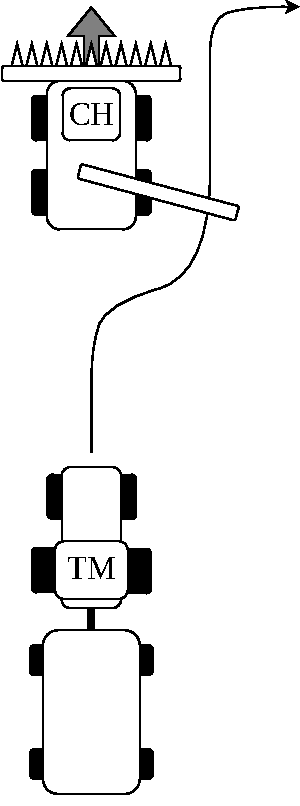
\includegraphics[width=0.21\textwidth]{figures/FieldExperimentDrive}
	\caption{Path around the static \acf{CH}, which the \acf{TM} will drive during the experiment to mimic various overloading positions}%
	\label{fig:fieldDrive}
\end{figure}

While driving along the specified path, the tractor will mimic various overloading positions, where shadowing effects can occur. After the tractor has passed the \ac{CH},
it will drive back to its starting position, and the experiment will be repeated with different overloading distances between the \ac{CH} and the tractor.

During the experiments, \ac{GPS} receivers at the agricultural machines will record the position and speed of the machines every \SI{1}{\second}.

The Wi-Fi setup consists of a Milesight Industrial Router UR75 \footnote{\url{https://iot-shop.de/en/shop/mil-ur75-500gl-g-p-w-milesight-ur75-500gl-g-p-w-industrial-cellular-5g-router-with-gps-wifi-and-poe-5677}}, which implements the standards IEEE 802.11 b/g/n in the \SI{2.4}{\giga\hertz} band and IEEE 802.11 a/n/ac in the \SI{5}{\giga\hertz} band and
IEEE 802.11 a/n/ac in the \SI{5}{\giga\hertz} band.
The router is equipped with two omnidirectional antennas for \SI{2.4}{\giga\hertz} and \SI{5}{\giga\hertz} usage.
\textcite{brinkhoff_characterization_2017} and \textcite{paul_characterizing_2011} already found out that placing the antenna higher above ground improves
the robustness and communication range of Wi-Fi networks in an outdoor environment.
As the regulation in the German Law StVZO §32 Abs. 2 limits the height of
every agricultural vehicle or combination of vehicles to less than \SI{4.0}{\metre}, the maximum antenna height is \SI{4}{\metre} above the ground. Therefore, I will mount the router on the tractor's roof at a height \SI{4}{\metre} above the ground.


I set up two Wi-Fi devices on the \ac{CH}, which are two UP Squared Boards \footnote{\url{https://eu.mouser.com/datasheet/2/826/UP_Square_DatasheetV0_4-3084829.pdf}} with an Intel AX210 Wi-Fi module \footnote{\url{https://docs.alfa.com.tw/datasheets/alfa-network_ait-ax210-ex_latest.pdf}}.

Every Intel AX210 Wi-Fi module supports the IEEE 802.11ax standard for \SI{2.4}{\giga\hertz}, \SI{5}{\giga\hertz} and \SI{6}{\giga\hertz} band and is equipped with two antennas,
which support omnidirectional transmissions in the \SI{2.4}{\giga\hertz}, \SI{5}{\giga\hertz} and \SI{6}{\giga\hertz} band and have a gain of \SI{5}{\decibel}.
The boards are mounted on the roof of the \ac{CH} next to one another at a height \SI{4}{\metre} above the ground too.

The router on the tractor sets up a Wi-Fi \ac{AP}.
One of the boards on the \ac{CH} connects to the \ac{AP} of the router as a Wi-Fi \ac{STA} and hosts an iperf3 \footnote{\url{https://iperf.fr/}} server.
A notebook is connected via LAN to the router and runs an iperf3 client, which connects to the iperf3 server on the \ac{CH}.
The iperf3 client sends \SI{100}{\byte} \ac{UDP} packets every \SI{100}{\milli\second} to the iperf3 server on the \ac{CH}.
The server records the received packets.
\textcite{paul_characterizing_2011} and \textcite{klingler_agriculture_2018} also used iperf3 to create \ac{UDP} traffic for their experiments.

Many different Wi-Fi transmissions arise through the iperf3 \ac{UDP} packets, the Wi-Fi manager of the Milesight Industrial Router, and the Intel AX210 Wi-Fi card.
These transmissions can be RTS/CTS, ACK, Data, Beacon or Probe request frame, displayed in \autoref{fig:fieldWifi}.
Through testing, I found out that the Wi-Fi manager of the Wi-Fi devices can apply \ac{VHT} \ac{MCS} \numrange{0}{9} and \ac{STBC} as physical layer configurations.

\begin{figure}[H]%
	\centering
	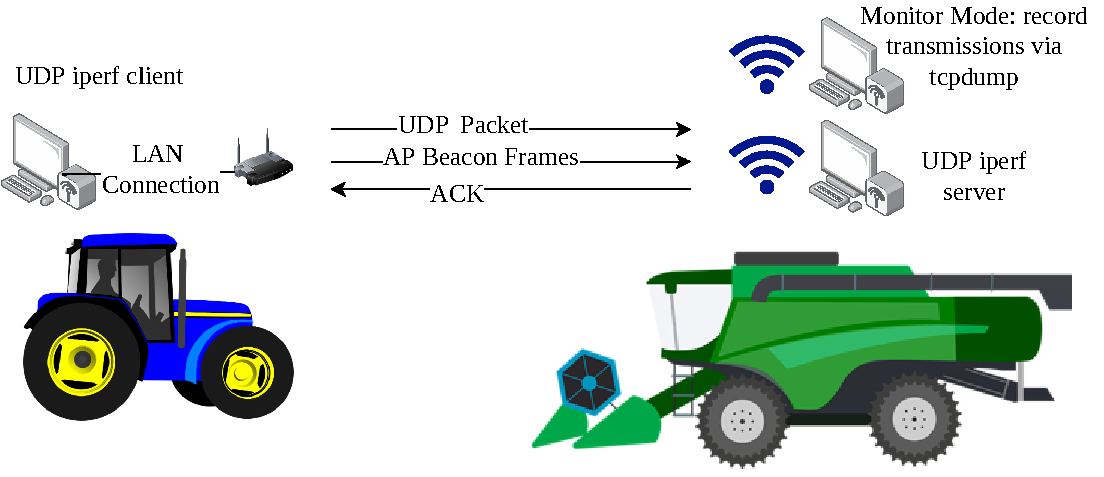
\includegraphics[width=0.98\textwidth]{figures/FieldExperimentwifi}
	\caption{Wi-Fi transmissions between the Wi-Fi \ac{AP} on the \acf{TM} and the Wi-Fi \ac{STA} on the \acf{CH}, which
	are recorded by a third Wi-Fi device in monitor mode on the \ac{CH}}
	\label{fig:fieldWifi}%
\end{figure}

The other UP Squared Board on the \ac{CH} uses the Wi-Fi card in the monitor mode and records every transmission in the \SI{5.6}{\giga\hertz} band using tcpdump \footnote{\url{https://www.tcpdump.org/}}.
Since the UP Squared board is placed next to the other board on the roof of the \ac{CH}, it can record the same signals the other board receives in the \ac{UDP} transmission.
The tcpdump records are in pcap - format, which can be analyzed using Wireshark\footnote{\url{https://www.wireshark.org/}}.
Using Wireshark, my plan is to identify possible retransmissions to calculate a \ac{PER}.
At the same time, the data contains the \ac{RSS} of each antenna and the physical layer parameters for every
transmission, allowing each transmission's robustness to be calculated as a function of the \ac{RSS} and the physical
layer configuration.

In order to get insights on the robustness of using the different frequency bands, the frequency channels for a \ac{BW} of \SI{20}{\mega\hertz} in \autoref{tab:fieldChannels} are configured.
To be able to calculate the means and standard deviations of the result for every configuration, the experiment is repeated \num{5} times for each channel,
which means that the tractor drives \num{5} times the same path, which is displayed in \autoref{fig:fieldDrive}.

\begin{table}[H]
	\centering
	\begin{tabular}{>{\centering}p{2cm}p{4cm}p{4cm}}
		\toprule
		\ac{BW} & Channel number \SI{2.4}{\giga\hertz} & Channel number \SI{5}{\giga\hertz}\\
		\midrule
		\SI{20}{\mega\hertz} & \num{1}&
		\num{100} \\
		\SI{40}{\mega\hertz} &
		\num{3}
		& \num{102} \\
		\SI{80}{\mega\hertz} &
		- & \num{106} \\
		\bottomrule
	\end{tabular}
	\caption{Frequency channel numbers for \SI{2.4}{\giga\hertz} and \SI{5}{\giga\hertz} for the different \acfp{BW} of the IEEE 802.11 standard \cite{ieee_standard_2021ax}, which can be used for
	outdoor communication \cite{freq_plan_24G}, \cite{freq_plan_5G} and can be configured in the Milesight Industrial Router UR75 for
	the field experiments.}
	\label{tab:fieldChannels}
\end{table}

\section{Trial Run}

To ensure that the experiment setup worked, I did a trial run and I got the data I needed as expected.
I mounted the Wi-Fi devices on the \ac{TM} and the \ac{CH} as shown in \autoref{fig:trailrunPositions} and
started the iperf3 client and server on the \ac{CH} and the \ac{TM} respectively.
During the trial run, the machines kept the same positions in a yard at the university.
To vary the recorded \ac{RSS}, I simultaneously moved the Wi-Fi antennas of the Wi-Fi devices on the \ac{CH} to
different positions.
I varied the used \ac{BW} of the \ac{AP} between \SIrange{20}{80}{\mega\hertz} in reference to \autoref{tab:fieldChannels}.
\begin{figure}[H]%
   \centering
   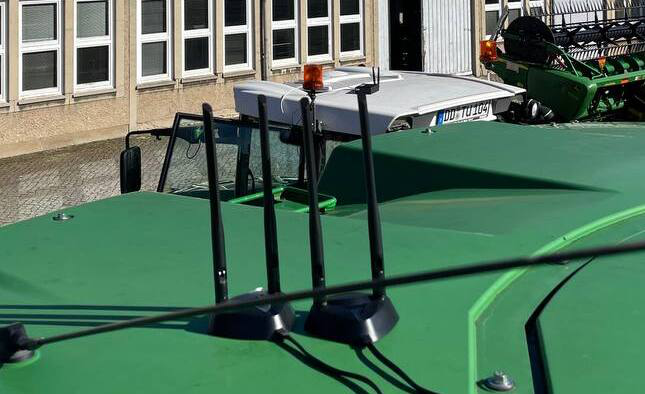
\includegraphics[width=0.5\textwidth]{figures/trainRun}
   \caption{Position of the Wi-Fi Devices on the \ac{TM} and the \ac{CH} during the trialrun}
   \label{fig:trailrunPositions}%
\end{figure}
The trial run was partly successful.
The monitoring Wi-Fi device blocked any try to configure monitoring channels with higher \ac{BW}s than \SI{20}{\mega\hertz}.
Therefore, I could only record data for a \ac{BW} of \SI{20}{\mega\hertz}.

The recorded data contains \ac{RSS}, physical layer configuration and MAC layer information of every received packet.
This can be used to find shadowing and fading effects, which may occur in the corn harvest scenario.

The recorded data was filtered to contain only the \ac{UDP} packets sent by the iperf3 client on the \ac{TM}
and displayed in \autoref{fig:trailrunIperf}.
It is visible that the Wi-Fi rate manager on the Milesight Industrial Router UR75 does not use \ac{STBC} and varies
the \ac{MCS} between \numrange{5}{8} and the \ac{GI} between \SIrange{400}{800}{\nano\second}.
Due to moving the antennas, the \ac{RSS} varies until I placed the antennas at a suitable fixed position at the end of the trial run.
As soon as the \ac{RSS} drops significantly at around \SIrange{25}{50}{\second}, the Wi-Fi rate manager switches to a lower \ac{MCS} and a longer
\ac{GI} to increase the transmission's robustness and reduce the retransmissions, which are indicated by the retry flag in the \ac{UDP} packet.

\begin{figure}[]%
   \centering
   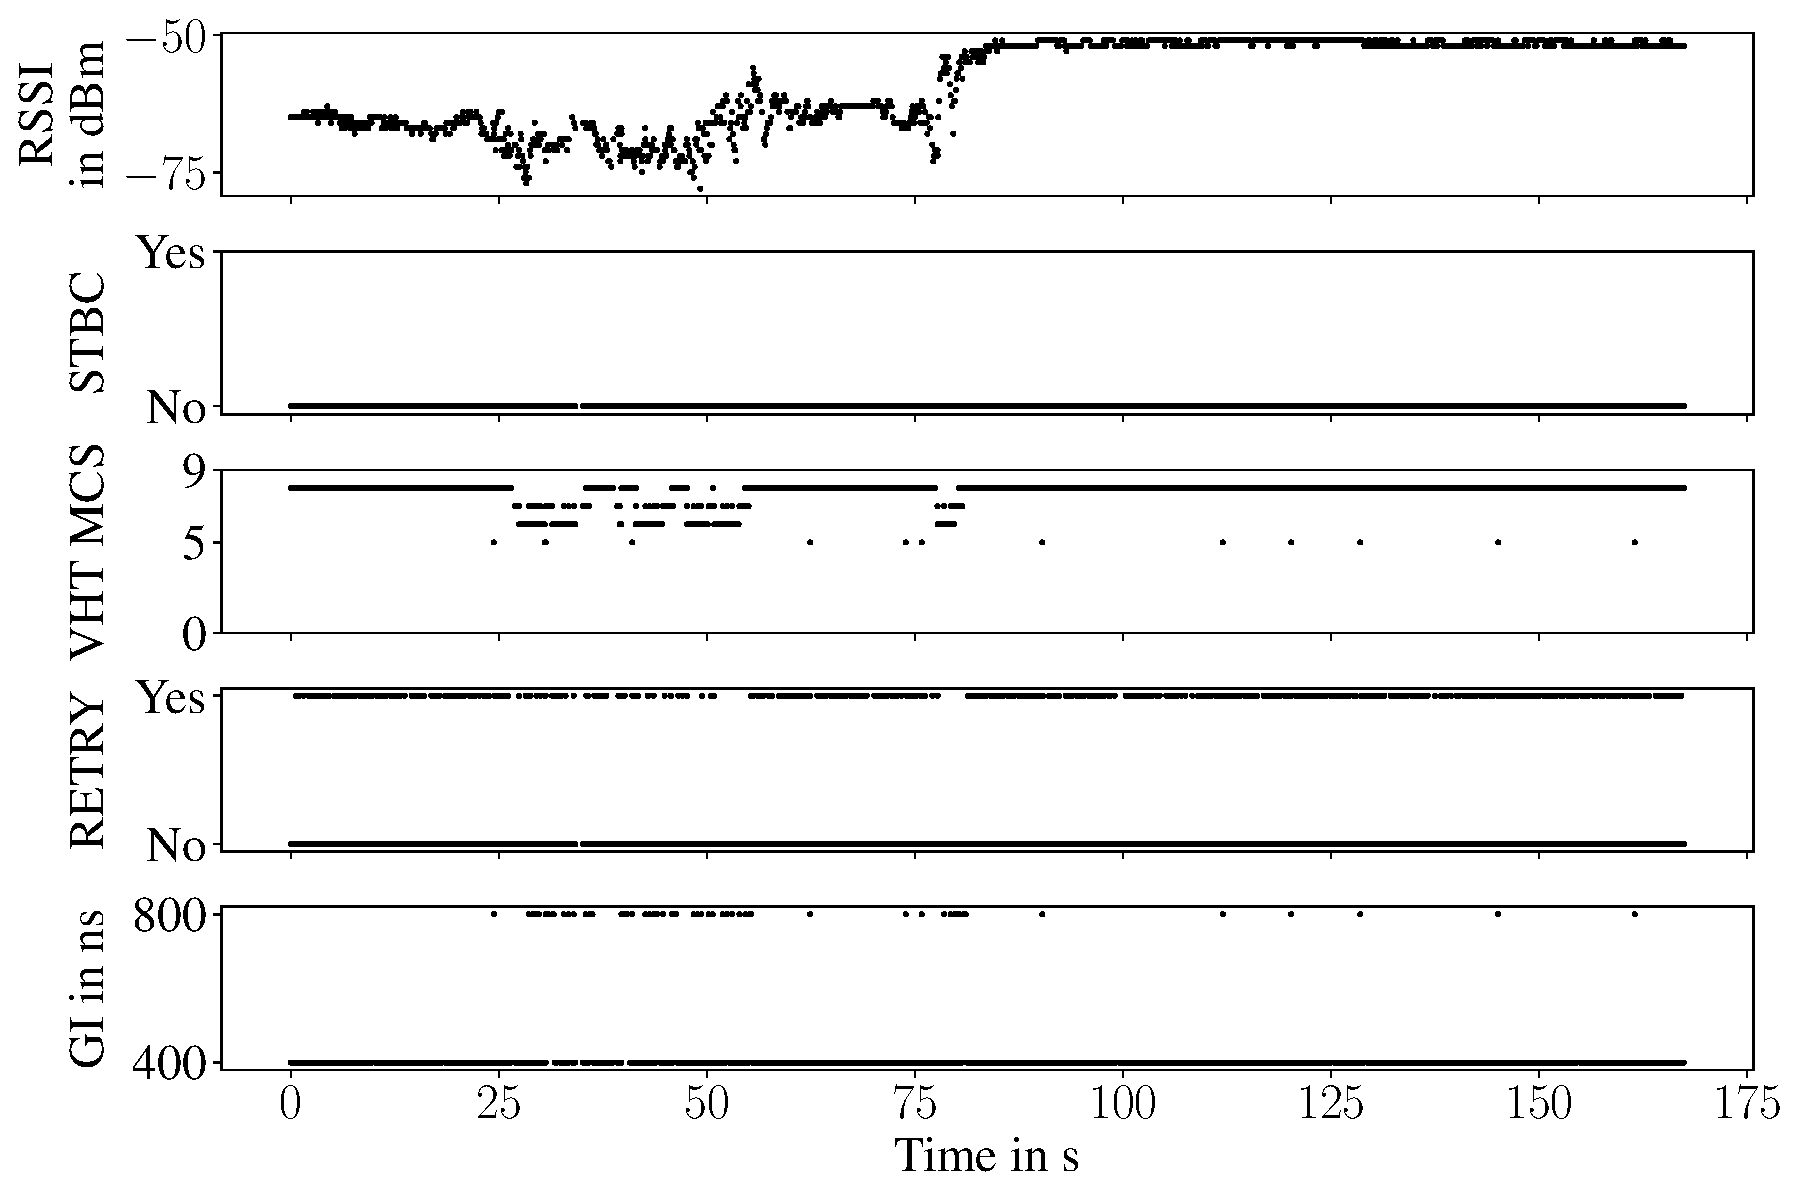
\includegraphics[width=0.95\textwidth]{figures/wireless5_144}
   \caption{All data transmissions between the Wi-Fi \acf{AP} on the \acf{TM} and the Wi-Fi \ac{STA} on the \acf{CH} in a trial run,
   which were initiated by the iperf3 client on the \acf{TM}}
   \label{fig:trailrunIperf}%
\end{figure}

The trial run took place in a yard at the university, where shadowing and fading effects due to buildings, trees, and agricultural machines are
expected.
The university ran other Wi-Fi networks, which may have interfered with my Wi-Fi network.
Therefore, many packets can get lost due to interference, shadowing or fading.

Every \ac{UDP} packet contains a sequence number to identify the packet.
If the packet is a retransmission, the packet contains the retry flag
with the same sequence number and data of the original transmission.
In general, \SI{25}{\percent} of received \ac{UDP} data packets contained retry flags.
This cannot be transferred to the \ac{PER} directly,
as it is unknown how many transmissions were sent by the iperf3 client and were lost due to interference, shadowing or fading.
To calculate the \ac{PER}, an additional Wi-Fi monitoring device next to the Wi-Fi router on the \ac{TM} is needed to record all
outgoing transmissions of the iperf3 client.
The \ac{PER} can then be calculated as the ratio of every successfully received \ac{UDP} packet to the number of transmitted \ac{UDP} packets.

Alternatively, retransmissions could be disabled as \textcite{klingler_agriculture_2018} did in their experiments.
Then every packet, which is missing in the sequence of received packets, is counted as a lost packet.
But the user interface of the Milesight Industrial Router UR75 has no option to disable retransmissions.

It is notable that the Wi-Fi rate manager on the Milesight Industrial Router UR75 always tries to use two spatial streams, the highest \ac{MCS} and the shortest \ac{GI} possible,
which results in the highest theoretical data rate.
For the \ac{BW} of \SI{20}{\mega\hertz}, the highest \ac{MCS} is \num{8} and the shortest \ac{GI} is \SI{400}{\nano\second} \cite{ieee_standard_2020}.
This translates to a theoretical data rate of \SI{173.3}{\mega\bit\per\second}, which is overdimensioned for the \ac{UDP} data packet rate of \SI{100}{\byte}
every \SI{100}{\milli\second}.
Additionally, the communication is less robust, which results in the high percentage of \SI{25}{\percent} of known retransmissions.

In the end, I could not conduct the proposed field experiments due to the rainy weather in the last \num{3} month of working period, which led to very wet agricultural fields.

\section{Wi-Fi Range Measurements}
Instead, I conducted a range measurement in an outdoor environment on an abandoned airfield near Mahlwinkel (52°23'17.9"N 11°50'35.4"E) in Saxony-Anhalt, Germany,
which can be seen in \autoref{fig:rangeEnvironment}.
The airfield was surrounded by grassland, wind turbines, a solar park and forests, which describe a typical environment for agricultural machines.
\begin{figure}[H]%
   \centering
   \includegraphics[width=0.75\textwidth]{figures/rangeMeasurementEnvironment}
   \caption{Airfield near Mahlwinkel (52°23'17.9"N 11°50'35.4"E) in Saxony-Anhalt, Germany, where I conducted the range measurements}
   \label{fig:rangeEnvironment}%
\end{figure}

I set up the Wi-Fi devices according to the setup above, where I replaced the \ac{CH} with a \SI{4}{\metre} wooden antenna mast and
the \ac{TM} with a roof extension on top of a car rack to reach a height of \SI{4}{\metre}.
The setup is shown in \autoref{fig:rangemeasurementSetup}.
\begin{figure}[]%
   \centering
   \includegraphics[width=0.75\textwidth]{figures/rangeMeasurementSetup}
   \caption{Setup of the Wi-Fi devices for the range measurements, which I mounted on wooden antenna masts to reach a height of \SI{4}{\metre}, the
   maximum allowed height of agricultural machines in Germany}
   \label{fig:rangemeasurementSetup}%
\end{figure}

The two Wi-Fi devices are mounted on the wooden antenna mast and were configured to run the iperf3 server and the monitoring mode.
I connected a \ac{GPS} receiver to the monitoring device and recorded the static position of the wooden antenna mast.
The wooden extension on top of the car rack carried the Wi-Fi router with the iperf3 client and an \ac{GPS} receiver to record the car's position every
second.

I place the Wi-Fi devices on the wooden antenna mast at one end of the airfield (52°23'17.8"N 11°50'41.7"E)
and drove the car with a speed of around \SI{10}{\kilo\metre\per\hour} (\SI{2.78}{\kilo\metre\per\hour}) the other end
of the airfield (52°23'17.8"N 11°50'29.7"E). Meanwhile, the iperf3 application exchanged \SI{100}{\byte} \ac{UDP} packets every
\SI{100}{\milli\second}.
Every Wi-fi transmission, which was received by the monitoring device, was recorded.
The iperf3 application ran while I drove away and back to the starting point.
I repeated this procedure three times to get a reliable result.

As I started the iperf3 client after the monitoring device, the first \ac{UDP} packets were recorded and used as a time reference to
synchronize the \ac{GPS} data of the car and the monitoring device.
I also used the recorded GPS time stamps to synchronize the recorded Wi-Fi transmissions with the \ac{GPS} logs.

\begin{figure}[]%
   \centering
   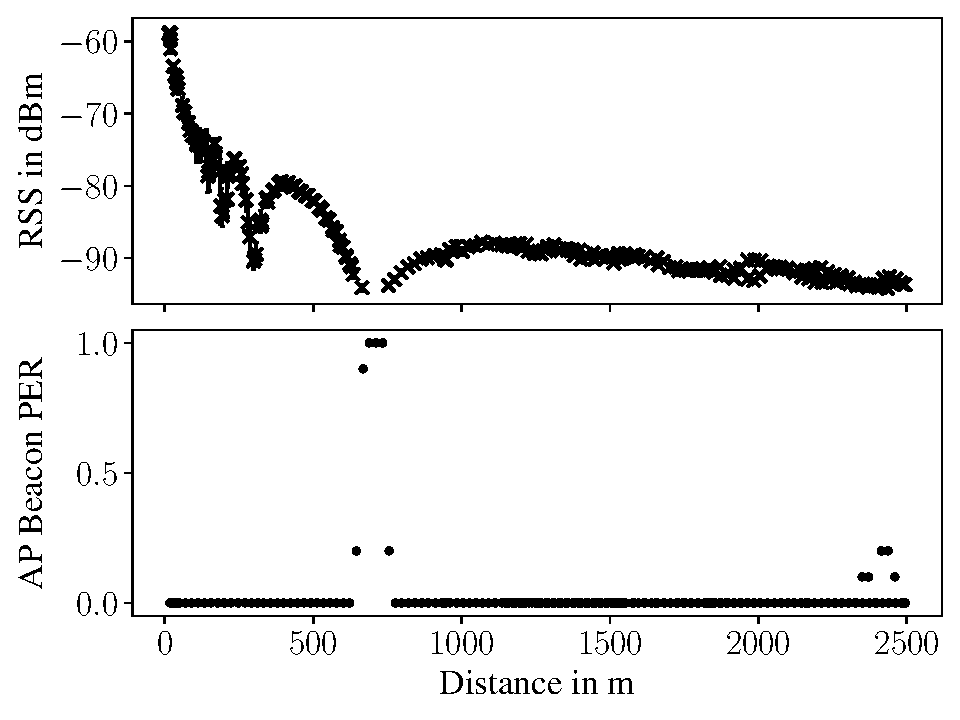
\includegraphics[width=0.8\textwidth]{figures/rangeMeasurementResults2}
   \caption{Range measurement results of the Wi-Fi transmissions on the airfield near Mahlwinkel (52°23'17.9"N 11°50'35.4"E) in Saxony-Anhalt, Germany}
   \label{fig:rangemeasurementResults}%
\end{figure}

The range measurement results are shown in \autoref{fig:rangemeasurementResults}.
I received Wi-Fi transmissions up to a distance of \SI{2.5}{\kilo\metre},
which equals the length of the airfield.

The \ac{RSS} values reflect a typical two-ray ground reflection model, where the ground reflection can be seen as a second ray,
which can cause destructive interference with the direct ray.
The destructive interference can be seen as the drops in the \ac{RSS} values.

At a distance of around \SIrange{650}{750}{\metre}, the \ac{RSS} values drop below the sensitivity of the Wi-Fi devices and
no Wi-Fi transmissions are received anymore.

This effect can also be detected in the \ac{PER} values of beacon frames.
The Milesight Industrial Router UR75 broadcasts every \SI{100}{\milli\second} the \ac{AP} beacon frame, which is used by Wi-Fi devices to
authenticate and associate with the \ac{AP}.
This beacon frame interval is defined in the recorded beacon frames and allows me to
calculate the \ac{PER} of the beacon frames as every \si{\second} \num{10} beacon frames should be received by the monitoring device.
The \ac{PER} of the beacon frames is shown in \autoref{fig:rangemeasurementResults} and indicates that no beacon frame was received at
a distance of around \SIrange{650}{750}{\metre}, because the \ac{RSS} values dropped below the sensitivity of the Wi-Fi devices.

\textcite{brinkhoff_characterization_2017} detected a similar effect at a range measurement with Wi-Fi on a rice field.
Inceasing the Antenna height,
resulted in a lower \ac{RSSI} values at a certain distance.
The authors explained this effect with the two-ray ground reflection on the water surface of the rice field,
which caused destructive interference with the direct ray.

The authors cite the following formula from \cite{rappaport_wireless_nodate} to find the distance, where local maxima
of destructive interference occurs and \ac{RSS} is at a minimum.
The distances $d$ can be calculated as a function of antenna heights
$h_r$ and $h_t$, the wavelength $\lambda$ and $k = 1, 2, 3, \dots$:
\begin{equation}\label{eq:destructiveInterference}
   \text{d} =
   \frac{
      2 \times h_r \times h_t
   }{
      \lambda \times k
   }
   \cdot
\end{equation}

Using \autoref{eq:destructiveInterference} with antenna heights of \SI{4}{\metre} and a wavelength of \SI{0.054}{\metre} for a frequency of \SI{5.6}{\giga\hertz},
the distances at which there are local minima of \ac{RSS} are \SI{199}{\metre}, \SI{299}{\metre}, and \SI{597}{\metre}.
The calculated distances are close to the measured distances of \SI{193}{\metre}, \SI{299}{\metre} and \SI{664}{\metre}.

This indicates that the measured effect is close to the theoretical two-ray ground reflection model.

Every beacon frame is transmitted in the IEEE 802.11a standard with a data rate of \SI{6}{\mega\bit\per\second}, which can also be received
by older Wi-Fi devices.
A data rate of \SI{6}{\mega\bit\per\second} refers to Binary \ac{PSK} modulation with a \ac{CR} of \nicefrac{1}{2} \cite{ieee_standard_1999}.
This \ac{MCS} and \ac{CR} combination is the most robust combination, which caused the low \ac{PER} values of the beacon frames over
the large communication range of up to \SI{2.5}{\kilo\metre}.
However, at the end of the communication range, the \ac{PER} values of the beacon frames
started to increase, because the \ac{RSS} values suffer more from fading effects and are not high enough to
to be sensed by the Wi-Fi devices.

\textcite{paul_characterizing_2011} conducted a similar range measurement with Wi-Fi devices across fields. Their
results for a continuous measurement over a distance of \SI{500}{\metre} revealed an approximate logarithmic decrease
in \ac{RSSI} values with increasing distance, with little two-ray ground reflection effects.
The satellite image of their measurement area shows a flat landscape with fields growing various crops.
In a second experiment, they measured a range of \SI{1. 8}{\kilo\metre} with a corresponding maximum throughput of
\SI{40.8}{\mega\bit\per\second}.

Similar to my range measurements the authors results indicate that long range Wi-Fi transmissions are possible. The achieved throughput of \SI{40.8}{\mega\bit\per\second} of
the authors leaves space for other physical layer configurations, which can be used to increase robustness and Wi-Fi range.

In general, \textcite{brinkhoff_characterization_2017} was also able to fit a logarithmic path loss model to their measurement results
for their Wi-Fi range measurement over different fields with different crops. However at the rice field, they detected
two-ray ground reflection effects from the water surface, which caused local maxima of destructive interference at certain distances.

This shows that my measurement results could have been different if I had done the range measurement in normal field.
The ground reflection effects would have been less significant, and the \ac{RSSI} values would have decreased logarithmically,
resulting in a lower \ac{PER} at a distance of \SIrange{650}{750}{\metre}.


The Wi-Fi rate manager on the Milesight Industrial Router UR75 used a \ac{VHT} \ac{MCS}0 for the \ac{UDP} data transmissions over this long communication distances, which also refers to a Binary \ac{PSK} modulation with a \ac{CR} of \nicefrac{1}{2}.
Additionally, it applied \ac{STBC} to increase the robustness of the Wi-Fi transmissions. This configuration resulted in a theoretical data rate of \SI{6.5}{\mega\bit\per\second} \cite{ieee_standard_2020}.

\section{Field Measurements Evaluation}

The achieved Wi-Fi transmission range may be dependent on the antenna height. \textcite{brinkhoff_characterization_2017} concluded that
the antenna height has a significant impact on the Wi-Fi transmission range.
They state, that the Wi-Fi transmission range increases
with the antenna height, because the Wi-Fi transmissions are less affected by obstacles and the Fresnel zone is less obstructed.
This effect is available until a maximum antenna height of \SI{50}{\metre} by the authors.

\textcite{krause_network_2021} performed simulations and measurements for network planning and coverage optimization
of mobile campus networks for agricultural and construction site scenarios.
They assume tractor heights of \SI{3. 5}{\metre} where an antenna can be mounted.
They conclude that higher antenna heights increase the fraction where a \ac{LOS} is available, resulting in
a higher data rate and less shadowing.

With regard to antenna height, future field experiments should be conducted to find the optimal antenna height for
agricultural machines.
Antenna masts can be built retractable and extendable to stay below the maximum allowed height of \SI{4}{\metre} for
agricultural machines on public roads in Germany and to be able to extend the antenna height to the optimal height
for the Wi-Fi transmission range in agricultural fields.

\ac{WIC} uses cases require reliable communication between the agricultural machines to exchange data
with each use case's specific required data rate, range, and latency.

The range measurements indicate that the Wi-Fi transmissions can be received up to a distance of \SI{2.5}{\kilo\metre},
which is sufficient to cover substantial agricultural fields.
However, Wi-Fi transmissions suffer from multipath, shadowing and fading effects, which can cause a large number of retransmissions,
when the physical layer configuration is oriented towards a high data rate instead of high robustness as it was
in the trial run.

As every used Wi-Fi device in the field experiment runs a Wi-Fi rate manager, which is responsible for the rate adaptation,
the influence of a particular physical layer parameter on the data goodput, robustness and latency can not be examined in the field experiment as no particular physical layer parameter can be set.
The Milesight Router is only capable of setting IEEE 802.11ac physical layer parameters, which don't include the new physical layer parameters of IEEE 802.11ax:
\ac{ER} mode, longer \ac{GI}s, \ac{HE}-\ac{MCS} \numrange{9}{11} or \ac{DCM}.

Taking \ac{DCM} as an example, the impact on the Wi-Fi receiver minimum input level sensitivity was mentioned in \autoref{fig:ReceiverSensitivityDCM}. \ac{DCM}
increases the robustness of the Wi-Fi transmissions and therefore allows a lower receiver minimum input level sensitivity to be used.

In the following chapter, I will analyze in simulations which physical layer
configurations are suitable for the agricultural environment to establish reliable communications,
which meets the data rate, range and latency requirements of Agricultural Platooning Services.







\chapter{Link Level Simulation}

Simulations benefit from the flexibility and possibility of simulating different communication and network protocols \cite{kumar_simulators_2012}.

Simulations are considered the main evaluation method for IEEE 802.11ax networks by the IEEE 802.11ax task group \cite{omar_survey_2016}.

The authors distinguish between link-level and system-level simulations for simulating \ac{HE} wireless networks.
The authors explain both methods as follows.

For system-level simulation, it requires abstractions of the physical and MAC layers to simulate a system close to
real on this basis.

Link-level simulations, according to the authors,
investigate the performance of the \ac{HE} physical layer for different physical layer parameters as \ac{PER} in terms of \ac{SNR}.
As an example, the authors cite multiple different researchers, which simulated \ac{PER} regarding \ac{SNR} and chosen \ac{MCS}.


\section{Robustness}
\label{sec:Robustness}
The field measurements showed.
\cite{smolnik_5g_2020} \SI{3}{\metre} corn plants
Therefore, the following section focuses on the influence of the different physical layer parameters on the robustness of the IEEE 802.11ax standard
Wi-Fi transmissions.

A known simulation tool for wireless communication networks is GNU Radio \footnote{https://www.gnuradio.org/}.
GNU Radio is an open-source software development toolkit, which has additional blocks for IEEE 802.11 network simulation,
called gr-ieee802-11 \footnote{https://github.com/bastibl/gr-ieee802-11}. However, the gr-ieee802-11 only
supports the IEEE 802.11a, IEEE 802.11b, IEEE 802.11g and IEEE 802.11p. This means, that the gr-ieee802-11 does not support
the \ac{ER} mode, \ac{DCM} or \ac{STBC}. Therefore, I decided that the GNU Radio is not suitable for my simulation.

\textcite{s_performance_2022} cites ns-3 \footnote{https://www.nsnam.org/docs/models/html/wifi-design.html},
that ns-3 does not implement
any frequency-selective fading effects, such as multipath propagation and shadowing. Therefore, the authors decided to use
the MATLAB WLAN Toolbox, which is standards-compliant and credible.
I also decided to use Matlab because besides \cite{s_performance_2022}, \cite{cao_efficient_2022} and \cite{jin_efficient_2021} have also considered
the MATLAB WLAN Toolbox to be suitable for IEEE 802.11ax simulations.

The MATLAB WLAN Toolbox \footnote{\url{https://de.mathworks.com/products/wlan.html?s_tid=AO_PR_info}} is a add-on to simulate, analyse, and test of wireless LAN communications systems.
The WLAN Toolbox supports a wide range of IEEE 802.11 standards.
Since Release R2019b \footnote{https://de.mathworks.com/help/wlan/release-notes.html}, the WLAN Toolbox supports the Signal Recovery, Packet Extension and Physical Layer abstractions to simulation IEEE 802.11ax networks.

My robustness analysis is based on the WLAN Toolbox example wlan/HESUExample \footnote{https://de.mathworks.com/help/wlan/ug/802-11ax-packet-error-rate-simulation-for-single-user-format.html} to simulate the \ac{PER} of point-to-point IEEE 802.11ax networks for
a specified \ac{SNR} values.

First, I set the IEEE 802.11ax physical layer parameters using the wlanHEConfig object,
where I define the default settings in \autoref{tab:robustnessDefaultSettings}.

\begin{table}
	\centering
	\begin{tabular}{>{\raggedright}p{4.5cm}p{4.5cm}}
		\toprule
		Parameter & Chosen Default Settings \\
		\midrule
		\ac{GI} & \SI{3200}{\nano\second} \\
		\ac{BW} & \SI{20}{\mega\hertz} \\
		Number Spatial Streams & \num{2}\\
		Number Transmit Antenna & \num{2} \\
		\ac{DCM} & disabled \\
		\ac{STBC} & disabled \\
		\ac{HE}-\ac{MCS} & \num{0} \\
		\ac{ER} & disabled \\
		\ac{LDPC} & enabled \\
		\bottomrule
	\end{tabular}
	\caption{Default physical layer settings for the IEEE 802.11ax robustness simulations}
	\label{tab:robustnessDefaultSettings}
\end{table}

Next, I chose a channel model to simulate the channel.
The WLAN Toolbox supports a wide range of channel models, such as wlanTGaxChannel, wlanTGnChannel, wlanTGacChannel, and wlanTGnChannel.
The wlanTGaxChannel model supports \num{6} different channel models for IEEE 802.11ax networks, named TGax-A, TGax-B, TGax-C, TGax-D, TGax-E, and TGax-F,
where the TGax-F channel model is suitable for pseudo-outdoor scenarios \cite{TGAXCHANNEL}.
The TGax channel models were used for Matlab Wlan Toolbox simulations by \cite{s_performance_2022}, \cite{cao_efficient_2022} and \cite{jin_efficient_2021}.

\cite{TGAXCHANNEL} and \cite{omar_survey_2016} list, that IEEE 802.11ax task group has also implemented the channel models UMa and UMi for
outdoor urban scenarios.
However, the WLAN Toolbox does not support these channel models and they are intended for urban scenarios, which

As I want to simulate outdoor scenarios, I chose the TGax-F channel model, which is suitable for pseudo-outdoor scenarios \cite{TGAXCHANNEL}.
The wlanTGaxChannel model supports configuring the \ac{BW}, the number of transmit and receive antennas, which I set equal to the configuration of the wlanHEConfig object.
\cite{freq_plan_24G} and \cite{freq_plan_5G} allow outdoor transmission in the frequency range of \SI{5.725}{\giga\hertz} to \SI{5.825}{\giga\hertz}. Therefore, I set the carrier frequency to \SI{5.6}{\giga\hertz}.
The TGax-F channel sampling rate is set to \SI{20}{\mega\hertz}, which is the nominal sampling rate for the configured \ac{BW} of \SI{20}{\mega\hertz}.
Additional parameters are left at their default values as they are not relevant for outdoor scenarios. According to the MATLAB WLAN Toolbox documentation \footnote{https://de.mathworks.com/help/wlan/ref/wlantgaxchannel-system-object.html},
the TGax-F channel model has a maximum delay of \SI{1050}{\nano\second} and root mean square delay spread of \SI{150}{\nano\second}.

The simulations is based on the procedure \autoref{alg:ProcedurePER}. To get a \ac{PER} for every \ac{SNR} value ranging
from \SIrange{0}{45}{\decibel}, the procedure \autoref{alg:ProcedurePER} is executed \num{5} times for \num{500} packets each.
All packet errors are counted and the \ac{PER} is calculated by dividing the number of packet errors by \num{500} packets.
A mean \ac{PER} and the confidence interval with a confidence level of
\SI{95}{\percent} is calculated of the \ac{PER} values of the \num{5} iterations.
\begin{algorithm}
\begin{algorithmic}[1]
\REQUIRE Global variable $numPacketErrors$
\STATE Create random packet data $txData$ of length \SI{1000}{\byte}
\STATE Create transmission waveform $txWaveform$ from packet data $txData$
\STATE $rxWaveform \gets $ $txWaveform$ passed through TGax channel model
\STATE Add noise to $rxWaveform$ based on \ac{SNR} value
\STATE Run packet detection on $rxWaveform$
\IF {no packet detected}
    \STATE $numPacketErrors \gets numPacketErrors + 1$
\ENDIF

\STATE Detect packet delay $delay$
\IF {$delay$ > \num{50} samples}
    \STATE $numPacketErrors \gets numPacketErrors + 1$
\ENDIF
\STATE Steps to recover packet data $rxData$ from $rxWaveform$
\IF {$txData$ != $rxData$}
    \STATE $numPacketErrors \gets numPacketErrors + 1$
\ENDIF
\end{algorithmic}
\caption{Procedure to detect packet errors}
\label{alg:ProcedurePER}
\end{algorithm}

The procedure \autoref{alg:ProcedurePER} starts with the creation of a random packet of the specified length of \SI{1000}{\byte}.
The packet is used to create a Wlan waveform based on the physical layer parameters specified in the wlanHEConfig object using the wlanWaveformGenerator function.

The waveform is extended by
\num{50} trailing zeros to ensure, that packet delays can be detected by finding trailing samples unequal to null. When the possible maximum detectable channel delay can be calulated by
\begin{equation}\label{eq:DELAY_CHANNEL}
	\text{detectable channel delay} =
	\frac{
		\text{Length of trailing zeros}
	}{
		\text{Sampling rate}
	}
	,
\end{equation}
then \num{50} trailing zeros match a maximum channel delay of \SI{2.5}{\micro\second}. As the maximum channel delay of the TGax-F channel model is \SI{1.05}{\micro\second},
\num{50} trailing zeros are sufficient to detect the maximum channel delay. I verified \autoref{eq:DELAY_CHANNEL} by comparing
the length of the maximum detected packet delay with the maximum channel delay of the TGax-F channel model. The results showed,
that maximum detected packet delay is \num{11} samples, which can be transfered using \autoref{eq:DELAY_CHANNEL} to rounded maximum TGax-F channel delay of \SI{1.1}{\micro\second}.

After creating the waveform an appending the trailing zeros, the waveform is passed through the TgaxF channel model to simulate the channel.
The output of the channel model is the received waveform, where I added noise to the transmitted waveform based on the
specified \ac{SNR} value and active \ac{OFDM} subcarriers.

The generated waveform is then passed through the configured wlanTGaxChannel to simulate the channel. The output of the channel model is the received waveform, where
I added additive white gaussian noise to the transmitted waveform based on the specified \ac{SNR} value.

In the next step, the received waveform is passed through the packet detection algorithm, which is based on the
WLAN Toolbox example wlan/HESUExample \footnote{https://de.mathworks.com/help/wlan/ug/802-11ax-packet-error-rate-simulation-for-single-user-format.html} and
shown in an abstracted form in \autoref{alg:PacketDetection}. The procedure calls various functions to decode the preamble, header and payload of
the received waveform. A packet error is detected, when, no packet can be detected, the packet delay is greater than \num{50} samples or the recovered packet data
is not equal to the transmitted packet data.

\subsubsection*{\acf{MCS} and \acf{CR}}
In a first simulation run, I analysed the influence of a chosen set of HE-MCS values on the \ac{PER} in regards to the \ac{SNR}.
The results in \autoref{fig:PER_SNR_MCS} show that the \ac{PER} decreases with higher \ac{SNR} for all HE-MCS values. The
\ac{PER} decreases at lower \ac{SNR} values for lower HE-MCS values. Increasing the HE-MCS value by \num{2} increases the \ac{SNR}, where a \ac{PER} of less than
\SI{10}{\percent} is achieved, by \SIrange{5}{6}{\decibel}.
\begin{figure}[H]%
	\centering
	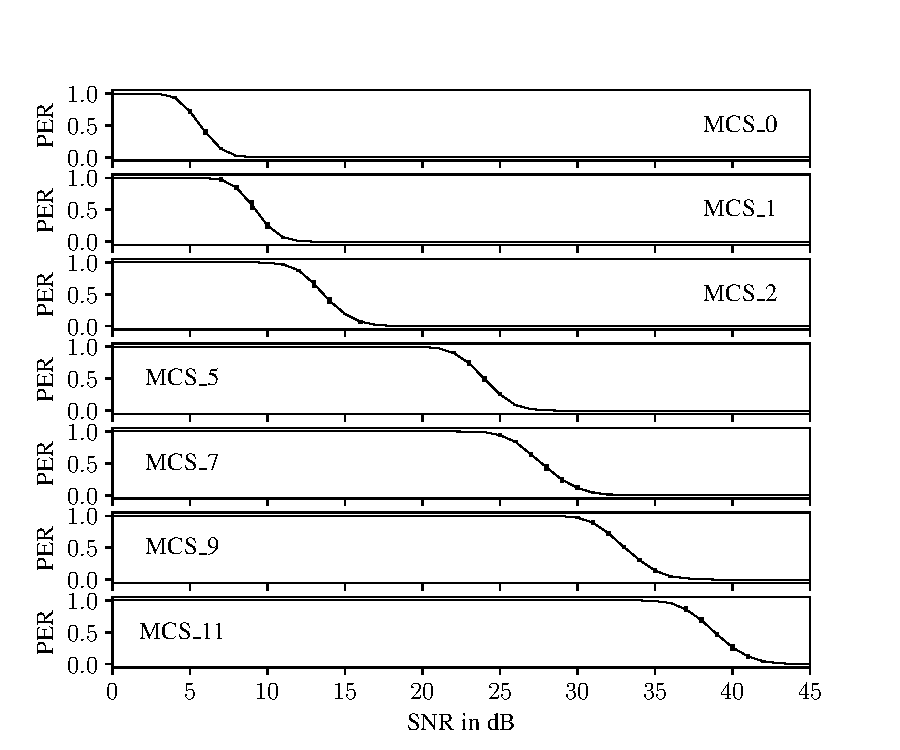
\includegraphics[width=0.95\textwidth]{figures/MCS_PER_to_SNR.pdf}
	\caption{Simulated PER in regards to SNR for chosen HE-MCS values for IEEE 802.11ax physical layer parameters
			of a GI of 3200 ns, a bandwidth of 20 MHz and 2 spatial streams.}
	\label{fig:PER_SNR_MCS}%
\end{figure}
\textcite{paul_characterizing_2011} conducted outdoor experiments to analyse the error rate and \ac{SNR} of different IEEE 802.11n \ac{MCS} for the
communication distances of \SI{300}{\meter}, \SI{800}{\meter} and \SI{1800}{\meter}. Their results show that \ac{SNR} decreases, when the transmissions range is longer.
Additionally, they experienced a higher error rate for higher.

The effect, that the \ac{PER} decreases, when the a lower \ac{MCS} or \ac{CR} is used, is the basis for the design of wifi rate managers.
A rate manager is a software component responsible to select physical layer parameters, such as \ac{MCS} or \ac{CR}, based on the current network conditions to
achieve the best possible throughput. Known rate managers of the linux kernel are the minstrel or the minstrel HT rate manager.

\subsubsection*{\acf{FEC}}
Another parameter that influences the \ac{PER} is the choice of the forward error correction (FEC) procedure. In order to
analyse the influence of the FEC procedure on the \ac{PER}, I simulated the \ac{PER} in regards to the \ac{SNR} for HE-MCS
\numrange{0}{9} and whether \ac{LDPC} or \ac{BCC} is enabled. For higher HE-MCS values \ac{BCC} can be used as \ac{LDPC} is compulsory, so no comparison of the \ac{FEC} procedures is possible.

The results are displayed in \autoref{fig:PER_SNR_LDPC}. The \ac{PER} decreases with higher \ac{SNR} for both \ac{FEC} procedures for all HE-MCS values as
expected. Using \ac{LDPC} instead of \ac{BCC}, a \ac{PER} of less than \SI{10}{\percent} can be achieved at \SI{2}{\decibel} higher \ac{SNR}
for all HE-MCS values. The effect increases to \SI{3}{\decibel} with higher HE-MCS values than HE-MCS \num{5}.
\begin{figure}[H]%
	\centering
	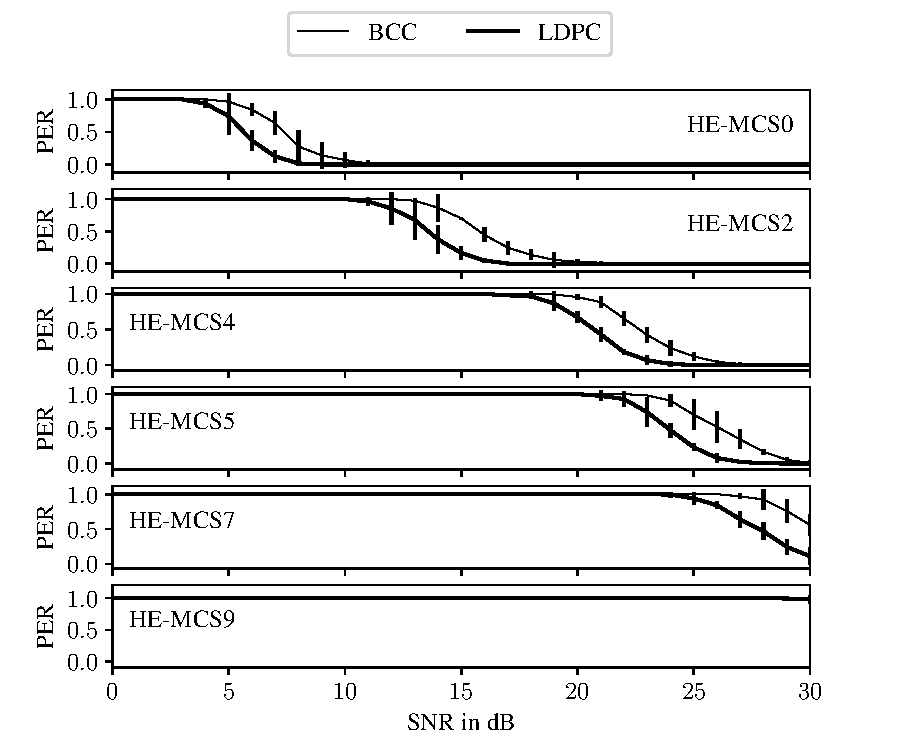
\includegraphics[width=0.95\textwidth]{figures/LDPC_PER_to_SNR.pdf}
	\caption{Simulated \ac{PER} in regards to \ac{SNR} for chosen HE-\ac{MCS} values and whether \ac{LDPC} or \ac{BCC} is enabled for IEEE 802.11ax physical layer parameters of a \ac{GI} of \SI{3200}{\nano\second}, a bandwidth of \SI{20}{\mega\hertz} and 2 spatial streams}%
	\label{fig:PER_SNR_LDPC}%
\end{figure}

\textcite{syafei_performance_2009} simulated the effect of the \ac{FEC} procedure on the \ac{PER} for IEEE 802.11n. They
had similar results and state, that using \ac{LDPC} instead of \ac{BCC}, a \ac{PER} of \SI{0.1}{\percent}  can be achieved at a
\SIrange{3.2}{6}{\decibel} higher \ac{SNR}.

According to \textcite{tran_asic_2014}, this effect is also present for IEEE 802.11ac. A \ac{PER} of \SI{0.1}{\percent} can be achieved at a
\SI{1.1}{\decibel} higher \ac{SNR} for using \ac{LDPC} instead of \ac{BCC} for 64 - \ac{QAM}. The effect increases to \SI{1.5}{\decibel} for 256 - \ac{QAM}.

\subsubsection*{\acf{GI}}

Robustness against intercarrier interference and intersymbol interference can be achieve by using a longer \ac{GI} \cite{pulimamidi_development_2007}. In order to analyse the impact of the \ac{GI} on the \ac{PER},
I simulated the \ac{PER} in regards to the \ac{SNR} for different HE-MCS values. The results for a \ac{GI} of \SI{3200}{\nano\second} and \SI{800}{\nano\second} are plotted in \autoref{fig:PER_SNR_GI}.
The \ac{PER} decreases with higher \ac{SNR} for all HE-MCS values as expected. Using a \ac{GI} of \SI{3200}{\nano\second} instead of \SI{800}{\nano\second} no significant difference of \ac{PER} in regards to the \ac{SNR} can be observed for HE-\ac{MCS} values lower than \num{5}.
Increasing the HE-\ac{MCS} value, the robustness of the \ac{MCS} sinks and the effect of the intercarrier interference and intersymbol interference increases.
As the maximum channel delay for the Tgax-F channel model is \SI{1050}{\nano\second}, the channel delay can be longer than the \ac{GI} of \SI{800}{\nano\second}. This
can result in intersymbol interference, which results in a higher \ac{PER} for higher HE-\ac{MCS} values.
For HE-\ac{MCS}\num{5}, a \ac{PER} of less than \SI{10}{\percent} can be achieved at \SI{1}{\decibel} lower \ac{SNR} for a \ac{GI} of \SI{3200}{\nano\second} instead of \SI{800}{\nano\second}. The effect increases
with higher HE-\ac{MCS} values.

\begin{figure}[H]%
	\centering
	
\includegraphics[width=0.95\textwidth]{figures/GI_PER_to_SNR.pdf}
	\caption{Simulated \ac{PER} in regards to \ac{SNR} for chosen HE-\ac{MCS} values and whether a \ac{GI} of \SI{800}{\nano\second} or \SI{3200}{\nano\second} is enabled for IEEE 802.11ax physical layer parameters of a bandwidth of \SI{20}{\mega\hertz} and 2 spatial streams}%
	\label{fig:PER_SNR_GI}%
\end{figure}
\textcite{patil_ieee_2020} conducted similar simulations for IEEE 802.11n.
They agree, that a longer \ac{GI} can increase the robustness against longer delay spreads as they are in the TGn-E and TGn-F channel models,
which are predecessors of the TGax-F channel model \cite{TGAXCHANNEL}.
\begin{comment}
	cite others seane old?? Evelt Van Duc Nguyen, 2016

\end{comment}



\subsubsection*{\acf{DCM}}
Next, I simulated the \ac{PER} in regards to the \ac{SNR}  and whether \ac{DCM} is enabled for the specfied HE-\ac{MCS} values. Dabei habe ich für die SImulation die möglichen
HE-MCS \num{0},\num{1},\num{3} and \num{4} aus dem IEEE 802.11ax Standard verwendet.

The results indicate, that using \ac{DCM} can achieve the same \ac{PER} at lower \ac{SNR} values compared to not using \ac{DCM}. A \ac{PER} of less than \SI{10}{\percent} can be achieved at
a \SI{2}{\decibel} lower \ac{SNR} when using \ac{DCM}.
The effect increases to \SI{4}{\decibel} for higher HE-\ac{MCS}\num{4}.
The results are plotted in \autoref{fig:PER_SNR_DCM}.
\begin{figure}[H]%
	\centering
	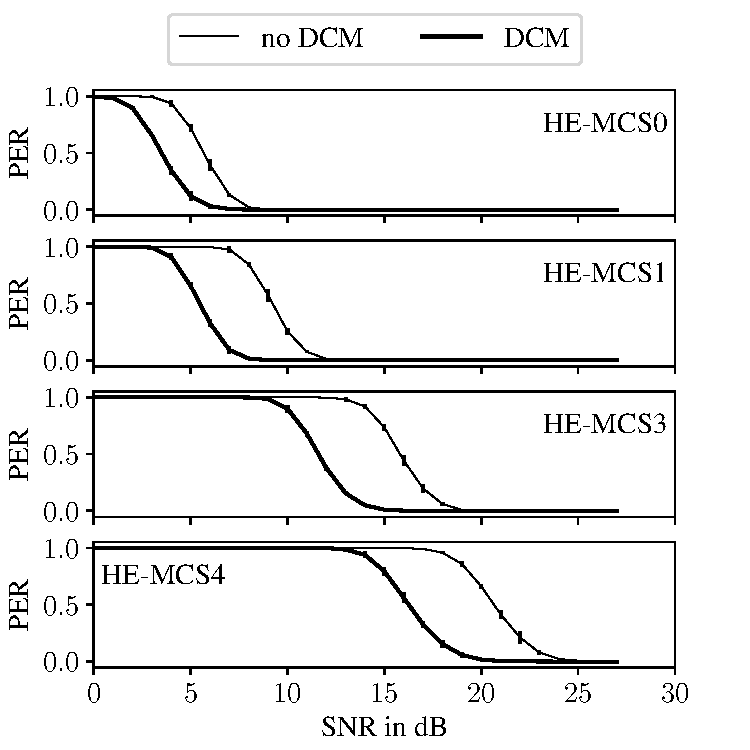
\includegraphics[width=0.95\textwidth]{figures/DCM_PER_to_SNR.pdf}
	\caption{Simulated \ac{PER} in regards to \ac{SNR} for chosen HE-\ac{MCS} values and whether \ac{DCM} is enabled for IEEE 802.11ax physical layer parameters of a \ac{GI} of \SI{3200}{\nano\second}, a \ac{BW} of \SI{20}{\mega\hertz} and 2 spatial streams}%
	\label{fig:PER_SNR_DCM}%
\end{figure}


\Textcite{ryu_ber_2010} and \textcite{park_ber_2006} conducted a similar simulation, where they analyse the bit error rate in
regards to the normalized \ac{SNR} and whether \ac{DCM} was enabled for rayleigh fading channels. Both authers wraped two
Quadrature \ac{PSK} modulated symbols into one 16-\ac{QAM} symbol. As Quadrature \ac{PSK} modulates \SI{2}{\bit} per symbol, the infomation
of two Quadrature \ac{PSK} modulated symbols can be
transmitted in one 16-\ac{QAM} symbol, which encodes \SI{4}{\bit}. The authors transmit the 16-\ac{QAM} symbols and a redundant copy
of the 16-\ac{QAM} symbols via orthogonal subcarriers. At the receiver the authors combine the copies and retrieve the transmitted
information using the Maximum likelyhood criterion. The results of the author show that a better bite error rate can be achieved while applying
\ac{DCM} than sending the information via two Quadrature \ac{PSK} or 16-\ac{QAM} modulated symbols without \ac{DCM}.
\cite{khorov_ieee_2015} DCM 2db gain


\subsubsection*{\acf{ER}}
For a HE-MCS \num{0} and \num{1} the \ac{ER} range mode can be applied additional to \ac{DCM}, when one spatial stream is used \cite{noauthor_ieee_2021}.
In order to analyse the impact of the \ac{ER} mode, I set the physical layer parameters to a \ac{GI} of
\SI{3200}{\nano\second}, a \ac{BW} of \SI{20}{\mega\hertz} and one spatial streams. For He-MCS \num{0}, \num{1} and \num{3} I run simulations, where I enabled the
\ac{ER} mode and compared the \ac{PER} to the \ac{PER} of the same HE-MCS values without \ac{ER} mode.

The results in \autoref{fig:PER_SNR_ER} indicate , that the \ac{PER} is influenced by the \ac{ER} mode.
The difference in \ac{SNR} with \ac{ER} mode to without \ac{ER} mode, where a \ac{PER}
of \SI{10}{\percent} is achieved, is \SIrange{1}{2}{\decibel}.
\begin{comment}
	{'mcs0_1_er.csv': [7.0, 6.0, 3.0], 'mcs1_2_er.csv': [11.0, 10.0, 6.0], 'mcs2_3_er.csv': [16.0, 14.0]}
\end{comment}
\begin{figure}%
	\centering
	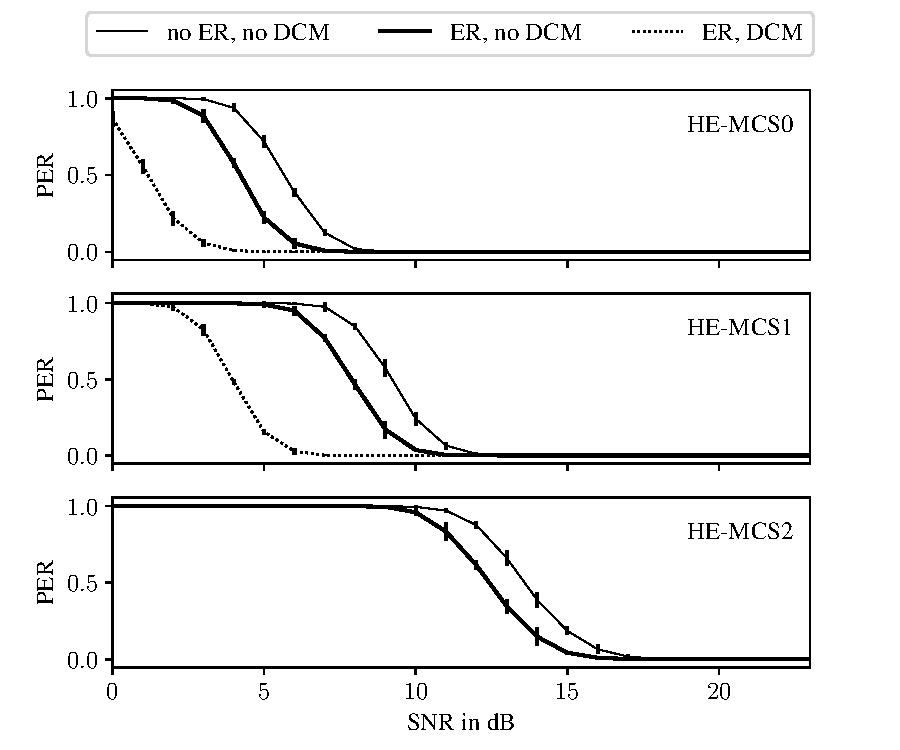
\includegraphics[width=0.95\textwidth]{figures/ER_PER_to_SNR.pdf}
	\caption{Simulated \ac{PER} in regards to \ac{SNR} for chosen HE-\ac{MCS} values and whether Extended Range or \ac{DCM}
	is enabled for IEEE 802.11ax physical layer parameters of a \ac{GI} of \SI{3200}{\nano\second}, a \ac{BW} of \SI{20}{\mega\hertz} and 2 spatial streams}
	\label{fig:PER_SNR_ER}%
\end{figure}

Additionally, I simulated the impact of applying the \ac{ER} mode and \ac{DCM} for the allowed HE-MCS values \num{0} and \num{1}.
Applying \ac{DCM} additionally makes the transmission more robust. As it is displayed in \autoref{fig:PER_SNR_ER_DCM},
a \ac{PER} of less than \SI{10}{\percent} can be achieved at a \SIrange{4}{5}{\decibel} lower \ac{SNR} when using \ac{DCM} and \ac{ER} mode together instead
of using \ac{ER} mode alone.

\textcite{jacob_system-level_2020} conducted a simulation, where they analysed the effect of \ac{DCM} and \ac{ER} on the \ac{PER} for
IEEE 802.11bd in vehicular environments to the transmission range. The authors found out, that the using \ac{DCM} and \ac{ER} can
increase the transmission range for \ac{LoS} by \SI{65}{\percent} for a \ac{PER} greater than \num{0.1}. After additional analysis with higher
vehicle densities, the authors remark, that using \ac{DCM} and the \ac{ER} mode cause channel congestion in CSMA/CA based
networks with low bandwidths. The authors conclude, that the \ac{ER} mode and \ac{DCM} should be used for long range transmissions, where
the physical layer parameters can extend the transmission range significantly.

A similar simulation was conducted by \textcite{triwinarko_phy_2021}. The researchers state, that using \ac{DCM} and the
\ac{ER} mode results in better \ac{PER} performance at lower \ac{SNR} values in \ac{LoS} and non \ac{LoS} scenarios.

\subsubsection*{\acf{STBC}}
As aforementioned, additional robustness can be achieved by applying \ac{STBC}. In order to analyse the impact of \ac{STBC} on the \ac{PER} in regards to the \ac{SNR},
I run the simulation for the HE-MCS values \numrange{0}{11} with and without \ac{STBC}.

The results in \autoref{fig:PER_SNR_STBC} indicate, that the \ac{PER} is influenced
by the \ac{STBC} mode. A \ac{PER} of less than \SI{10}{\percent} is possible at a \SIrange{2}{10}{\decibel} lower \ac{SNR} when using \ac{STBC} additionally.
The impact of \ac{STBC} on the \ac{PER} grows from \SI{2}{\decibel} for HE-MCS\num{0} to \SI{10}{\decibel} for HE-MCS\num{11}.
\begin{comment}
	{'mcs0_stbc.csv': [7.0, 5.0], 'mcs2_stbc.csv': [16.0, 8.0], 'mcs9_stbc.csv': [36.0, 26.0],
		'mcs7_stbc.csv': [30.0, 20.0], 'mcs5_stbc.csv': [26.0, 18.0], 'mcs1_stbc.csv': [11.0, 6.0], 'mcs11_stbc.csv': [41.0, 31.0]}
\end{comment}

\begin{figure}%
	\centering
	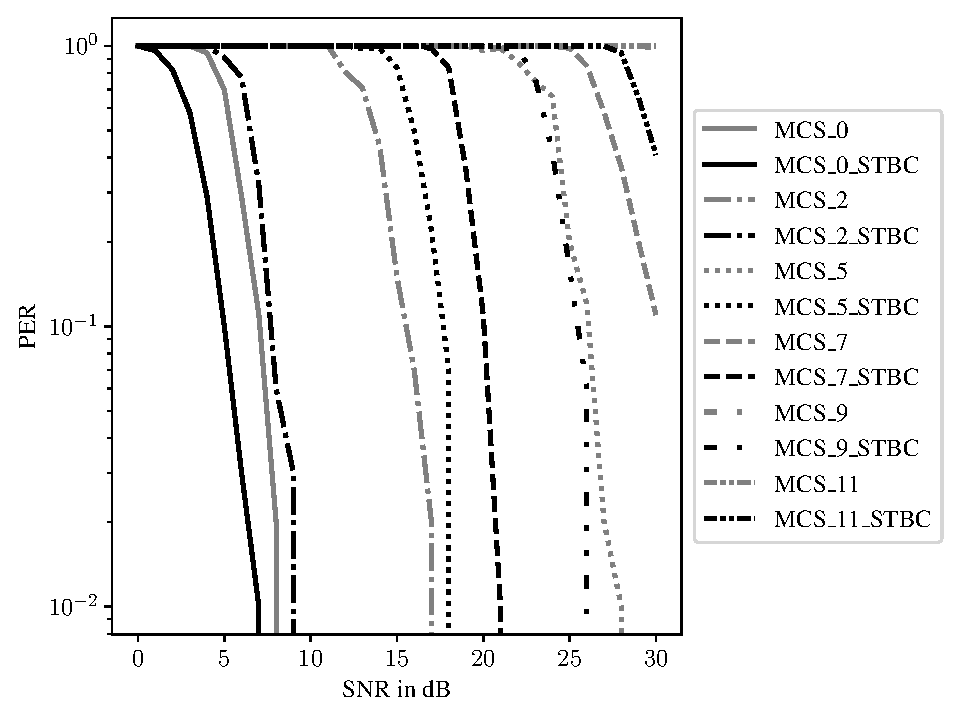
\includegraphics[width=0.95\textwidth]{figures/STBC_PER_to_SNR.pdf}
	\caption{Simulated \ac{PER} in regards to \ac{SNR} for chosen HE-\ac{MCS} values and whether \ac{STBC} is enabled for IEEE 802.11ax physical layer parameters of a \ac{GI} of \SI{3200}{\nano\second}, a \ac{BW} of \SI{20}{\mega\hertz} and 2 spatial streams}%
	\label{fig:PER_SNR_STBC}%
\end{figure}
\textcite{stamoulis_impact_2003} analysed the impact of \ac{STBC} on the bit error rate for IEEE 802.11a in regards to the \ac{SNR}. Their simulation was based
on a HiperLAN/2 channel with \num{2} antennas. They used HiperLAN/2, because it has a similar physical layer as IEEE 802.11a.
The authors found out, that applying \ac{STBC} results in a lower bit error rate for a given \ac{SNR} value. The authors conclude, that \ac{STBC} can be used to
\textcite{santumon_space-time_2012} and \textcite{tarokh_space-time_1999} conducted simulations, where they analysed the effect of \ac{STBC} on the bit error rate for
wireless communication systems. In general, the authors found out, that \ac{STBC} can be used to increase the bit error rate for a given \ac{SNR} value for different
\ac{MCS} values. Additionally, the authors remark, that the impact of \ac{STBC} on the bit error rate grows with the number of antennas.
However, the number of antennas is limited to \num{2} for IEEE 802.11ax \cite{noauthor_ieee_2021}.

The robustness analysis results indicate, which \ac{PER} decreases can be achieved by applying the different phsyical layer parameters.
The intensity of the impact varies depending on the environment and the actual communication channel.

I conducted the same simulations for the frequency band of \SI{2.4}{\giga\hertz}. Using the same physical layer parameters in
the \SI{2.4}{\giga\hertz} band achieve a similar \ac{PER} in regards to the \ac{SNR} and chosen physical layer parameters
as in the \SI{5}{\giga\hertz} band.

But how does the effect of the frequency bands on the \ac{PER} in regards to the \ac{SNR} differ?
Taking the Friis transmission model \cite{shaw_radiometry_2013} into account, the \ac{RSS} for omnidirectional antennas can be calculated in regard to the distance $d$,
receiving antenna gain $G_{R}$, transmitting antenna gain $G_{T}$ and transmission power $P_{T}$  as follows:
\begin{equation}
	RSS = P_{T} * G_{T} * G_{R} * \frac{\lambda^2}{(4 * \pi * d)^2}.
\end{equation}
When $\lambda$ is replaced and  $P_{T}$,  $G_{T}$,  and $G_{R}$ are set to \num{1} the following equation can be derived:
\begin{equation}
	RSS = \frac{c^2}{(f* 4 * \pi * d)^2},
\end{equation}
where $c$ is the speed of light and $f$ is the frequency of the transmission.
Converting the equation to $d$ it results in the following equation:
\begin{equation}
	d = \frac{c}{(4 * \pi * f * \sqrt {RSSI})}.
\end{equation}
The equation shows, that a lower frequency results in a higher \ac{RSS} for a given distance.
This means, that the \SI{2.4}{\giga\hertz} band can achieve a higher \ac{SNR} for a given distance and noise floor
compared to the \SI{5}{\giga\hertz} band.
The simulation results can now be used to derive the following conclusion,
that a lower \ac{PER} for the \SI{2.4}{\giga\hertz} band can be accomplished
for a given set of physical layer parameters, distance and noise floor.


\todo{What should be chosen?}

\section{Data Rate}
\label{sec:DataRate}
For the simulation of Wi-Fi data throughput, various tools are already available, such as Matlab, ns-2 and ns-3, OMNeT++, Qualnet \cite{keller_simulation_2021} or OPNet \cite{kumar_simulators_2012}.

\textcite{kumar_simulators_2012} compares different available simulators for the simulation of wireless networks and concludes that, in general, ns-2, ns-3 and OMNeT++ are the most popular simulators for academic research of wireless networks.
\textcite{keller_simulation_2021} mentions that ns-3 keeps a more accurate Implementation of the IEEE 802.11 standard than OMNeT++.
So far, I know that OMNeT++ supports some IEEE 802.11ac modes via the library INET Release 4.0.0 \footnote{\url{https://inet.omnetpp.org/2018-06-28-INET-4.0.0-released.html}}.
Consequently, OMNeT++ seems unsuitable for IEEE 802.11ax simulations and I looked at ns-3.


\subsubsection*{ns-3 Network Simulator}
\todo[color=yellow]{fundamentals of ns-3}
Ns-3 is well documented in the ns-3 manual in the \textit{./doc} - folder of  \cite{henderson_ns-3-dev_2023}, where I found the following information about the simulator.
Ns-3 is a discrete-event network simulator project which was founded in 2006.
The ns-3 project is open source with a licence based on GNU GPLv2 compatibility.
It aims to provide an open, extensible network simulator for research and educational use.
Ns-3 scripts can be written in C++ or Python.

The concept of ns3 is based on the abstraction of simulated systems.
For this purpose, the term node was introduced for basic computing devices.
The Node class offers the possibility of installing protocol stacks and applications or adding peripheral cards and mobility models to the node.
Applications are the abstraction of the user-level applications, representing an activity to be simulated.
For this purpose, the applications use resources and functionalities provided by the system software of a node.

Every node gets network access via the Net Device class.
The Net Device class represents the physical interface of a node,
which can be a network interface card or peripheral card.
The Net Device simulates the software driver and the network interface hardware.

Every Net Device is connected to a channel.
The channel class represents the physical medium which is used to transmit data.
The channel behaviour is based
on the channel model, which may include interference, propagation delay and loss.

The current version ns-3.37 supports IEEE 802.11ax as a standard in infrastructure and ad-hoc mode \footnote{\url{https://www.nsnam.org/docs/models/html/wifi-design.html}}.
However, support for the 802.11ax standard is not yet complete.
It is already possible to configure \ac{DCM} and \ac{STBC},
but there is a comment in line 496 of the file \textit{he-ppdu.cc} that these are
not yet taken into account in the current ns-3 version 3.37 \footnote{\url{https://www.nsnam.org/docs/models/html/wifi-user.html}}.

When examining the implementation of 802.11ax in ns-3, one notices that the implementation of 802.11ax in ns-3 already implements a \ac{HE} \ac{ER} SU \ac{PPDU} preamble, but this is never used, and one cannot activate the extended range mode.
Therefore, some open points of 802.11ax in ns-3 still need to be implemented.

\textcite{black_netsimulyzer_2021} have developed a 3D visualisation of ns-3, which visualises the simulations in 3D to make the ns-3 simulation
scenarios tangible.
The authors' graphical extension consists of two open source programmes.
The NetSimulyzer ns-3 module \footnote{https://github.com/usnistgov/NetSimulyzer-ns3-module} can be integrated into the ns-3 simulation and builds a JSON file using the specified functions and configurations.
This file contains all the data required for visualisation in the application NetSimulyzer \footnote{\url{https://github.com/usnistgov/NetSimulyzer}}.


Ns-3 is chosen as a simulation tool for the simulation of 802.11ax by \cite{dolinska_new_2019}, \cite{rochim_performance_2020} and
\cite{behara_performance_2022}.


As ns-3 is an open-source simulation software and was used by the mentioned other researchers in the past too, I used ns-3
to evaluate the effect of physical layer configuration on the achievable goodput between two nodes using IEEE 802.11ax Wi-Fi Netdevices
to exchange \ac{UDP} packets in ad-hoc Mode.

The setup consists of two nodes placed in static positions with a distance of \SI{20}{\metre}.
I chose the short communication range setup with no simulated interference to enable Wi-Fi transmission without any packets lost.

Every node is equipped with an IEEE 802.11ax Wi-Fi NetDevice, which is configured with the default parameters in
\autoref{tab:SimulationDataRate}.
\begin{table}[H]
   \centering
   \begin{tabular}{p{6cm}p{4cm}}
      General Parameters & \\
      \midrule
      Wi-Fi Standard & IEEE 802.11ax\\
      \ac{GI} & \SI{3200}{\nano\second}\\
      Frequency Spectrum & \SI{5.6}{\giga\hertz}\\
      \ac{BW} & \SI{20}{\mega\hertz}\\
      max. Transmission Power & \SI{25}{\decibel}\\
      Antenna Gain & \SI{5}{\dB}\\
      Spatial Streams & 2\\
      \bottomrule
   \end{tabular}
   \caption{Default simulation parameters for Wi-Fi Devices in the goodput simulations}
   \label{tab:SimulationDataRate}
\end{table}

A Constant Rate Wi-Fi Manager is used to set a constant data rate according to the fixed \ac{HE}-\ac{MCS} for data, non-uniform and control data transmissions.
The used frequency band is \SI{2.4}{\giga\hertz} or \SI{5}{\giga\hertz} as higher frequencies are less resistant to shadowing and fading, and a higher data rate is not needed for the \ac{WIC} use cases.
The Wi-Fi Netdevices operate in the frequency channels specified in \autoref{tab:fieldChannels}, which can be used for
outdoor Wi-Fi communication in Germany \cite{freq_plan_24G}, \cite{freq_plan_5G}.

The simulation is based on the ns-3 ConstantSpeedPropagationDelayModel and the  ns-3 FriisPropagationLossModel,
representing free-space signal propagation at the speed of light.
The FriisPropagationLossModel is suitable for outdoor scenarios with a clear \ac{LOS} between the nodes.
As both nodes are only \SI{20}{\metre} apart a transmission in the \ac{LOS} is possible.
The ns-3 TableBasedErrorRateModel is used to model the error rate of the physical layer.
According to the ns-3 Wi-Fi design guide \footnote{\url{https://www.nsnam.org/docs/models/html/wifi-design.html\#default-table-based-error-model-validation}},
the TableBasedErrorRateModel derives the \ac{PER} from results of the Matlab WLAN Toolbox
regarding the physical layer parameters and \ac{SNR}.
The design guide recommends the TableBasedErrorRateModel for the IEEE 802.11ax standard.

As the Wi-Fi standard implements ACKs for every packet, every lost packet is repeated until it is received or the number of retries is
exceeded.
Platooning Services are time critical, so the number of retries should be as low as possible.
This is why additional retransmission mechanisms like TCP are not needed.
Therefore, the chosen transport layer protocol is UDP.

One node operates a \ac{UDP} server, and the other is a \ac{UDP} client.
The client sends \SI{1000}{\byte} \ac{UDP} packets to the server every \SI{0.1}{\micro\second}.
This packet interval
ensures that the packet queue of the client is never empty after starting the simulation.
The server receives the packets and sends an ACK back to the client.

For every physical layer configuration, the simulation runs five times for \SI{5}{\second}.
The goodput for every simulation run is calculated by dividing the number of received bytes at the \ac{UDP} Server by the simulation time.
The goodput is then averaged over all simulation runs per physical layer configuration, and the confidence interval with a confidence level of
\SI{95}{\percent} is calculated.

The theoretical data rate for the different physical layer configurations is retrieved from the function ns3::WifiMode::GetDataRate().

To verify the simulation software, I used different methods.
First, I confirmed that the theoretical data rate for the simulation's IEEE 802.11ax physical layer configurations equals the theoretical data rate specified in the IEEE 802.11ax standard \cite{ieee_standard_2021ax}.

I also used the MonitorSnifferRxCallback and the MonitorSnifferTxCallback of the ns-3 WifiPhy class to check the ongoing transmissions.
Both Callback functions can be added to WifiPhy objects of Wi-FiNetDevice and are called every time a packet is received or transmitted at the Wi-Fi Netdevice.
The function parameters are information about the packet, channel frequency and station ID and an instance of the WifiTxVector class.
The WifiTxVector instance in the current ns-3 version 3.37 describes all parameters of the transmission in accordance to the TXVECTOR field of the IEEE 802.11 standard \cite{ieee_standard_2021ax}. Additionally, the function parameters of the MonitorSnifferRxCallback contain the signal strength and
the noise power of the received packet.

Using the provided information from the MonitorSnifferRxCallback and the MonitorSnifferTxCallback, I was able to comprehend the ongoing transmissions and
verify the simulation results.

\subsubsection*{\acf{GI}}

In the first simulation, I varied the \ac{GI} of the Wi-Fi Netdevices for different \ac{HE}-\ac{MCS} values.
The results are shown in \autoref{fig:Data_rate_GI}.
The achieved goodput is plotted against the theoretical data rate for the different \ac{GI} values.
The theoretical data rate is always higher than the achieved goodput of the \ac{UDP} applications because Wi-Fi devices
cannot transmit data during other ongoing transmissions and the corresponding \acp{IFS}.
These transmissions can be \ac{ACK} and ad-hoc Beacon transmissions.
Due to this waiting time, the goodput is lower than the theoretical data rate.
\begin{figure}[H]
   \centering
   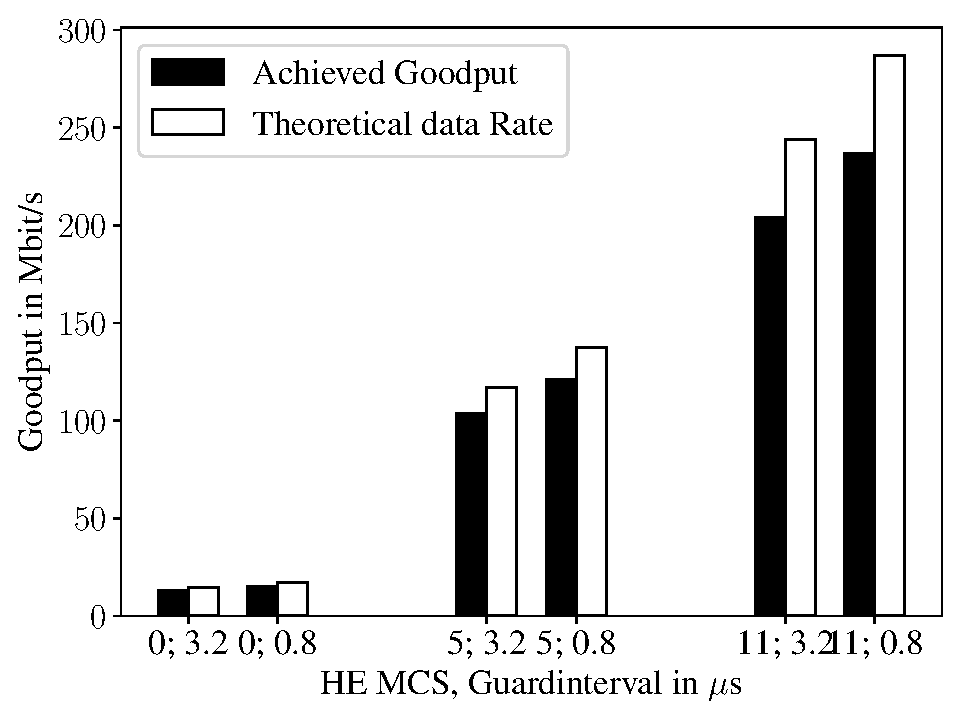
\includegraphics[width=0.64\textwidth]{figures/gi_dataRate_simulation.pdf}
   \caption{Achieved Goodput and theoretical Datarate of two Wi-Fi6 stations in Ad-Hoc Mode
   with \num{2} \acf{MIMO} streams and a bandwidth of \SI{80}{\mega\hertz} in regards to the chosen \acf{GI} and \ac{HE}-\ac{MCS} value}%
   \label{fig:Data_rate_GI}%
\end{figure}

The achieved goodput decreases as the \ac{GI} length increases.
This effect can be characterized by \autoref{eq:GI}.
The bandwidth attenuation for the possible \ac{GI} lengths is displayed in \autoref{tab:GIbandwidthAttenuation}.
The effect of the bandwidth attenuation for the different \ac{GI} lengths can be observed in the mean achieved goodput in
\autoref{tab:GIbandwidthAttenuation}, where the decrease of the mean goodput reflects the bandwidth attenuation of the decreasing \ac{GI} length.

A similar effect can be observed with higher \ac{HE}-\ac{MCS} values.
\begin{table}[H]
   \centering
   \begin{tabular}{>{\centering}p{3cm}p{3cm}p{3cm}}
      \toprule
      \ac{GI} & Mean achieved goodput & \ac{BW} attentuation\\
      \midrule
      \SI{800}{\nano\second} & \SI{31.15}{\giga\bit\per\second}&
      \SI{94}{\percent} \\
      \SI{1600}{\nano\second} &
      \SI{29.47}{\giga\bit\per\second}&
      \SI{89}{\percent} \\
      \SI{3200}{\nano\second} & \SI{26.52}{\giga\bit\per\second}&
      \SI{80}{\percent} \\
      \bottomrule
   \end{tabular}
   \caption{\acf{BW} attenuation and mean goodput for \ac{HE}-\ac{MCS}0 in regards to \acf{GI} length}
   \label{tab:GIbandwidthAttenuation}
\end{table}

\textcite{patil_ieee_2020} and \textcite{karmakar_s2-gi_2020} conducted similar simulations
for the \SI{400}{\nano\second} and \SI{800}{\nano\second} \ac{GI} lengths in IEEE 802.11n and IEEE 802.11ac, respectively.
Both papers state that shorter \ac{GI} lengths lead to higher goodput values under the condition that there is a short delay spread and a low
channel loss due to interference.

\subsubsection*{\acf{ER} Mode}

In the following simulation, I analyzed the effect of the \ac{ER} Mode on the goodput of the IEEE 802.11ax physical layer.
As mentioned in ns-3 Version 3.37, the \ac{ER} Mode is implemented as a \ac{HE} Capability with the new extended WifiPreamble.
But the new preamble in the \ac{HE} \ac{ER} SU \ac{PPDU} format is not used in ns-3 version 3.37.

As I was using the ConstantRateWifiManager, all parameters for the data transmission are set in the function
ConstantRateWifiManager::DoGetDataTxVector().
The function creates a WifiTxVector instance with the parameters of the
transmission.
There I overwrote the preamble type to the already implemented ns3 WifiPreamble::WIFI\_PREAMBLE\_HE\_ER\_SU, when
the \ac{ER} Mode is enabled and conditions for the \ac{ER} Mode in the IEEE 802.11ax standard \cite{ieee_standard_2021ax} are fulfilled.
Ns-3 version 3.37 implements the ns3::GlobalValue, which allows users to set global values for the simulation, which can be accessed
in every class without changing Constructor or function parameters.
This leaves the original functionality of the ns3 code intact.

I used the ns3::GlobalValue to create an instance named HE\_ER\_Mode, which is set to true at the start and read in the ns3::ConstantRateWifiManager::Do\-Get\-Data\-Tx\-Vector() function
to overwrite the preamble type.

Via the MonitorSnifferRxCallback and the MonitorSnifferTxCallback, I was able to verify that the ns3 WifiPreamble::WIFI\_PREAMBLE\_HE\_ER\_SU was used
for data transmission, when the following conditions were met: a) the \ac{ER} Mode is enabled, b) the number of spatial streams is \num{1}, c) the \ac{HE}-\ac{MCS} value is less than \num{3} and
d) the \ac{BW} is \SI{20}{\mega\hertz}.

The simulation results are shown in \autoref{fig:Data_rate_ER}, where the reduction of achieved goodput is plotted against the theoretical data rate for the different \ac{HE}-\ac{MCS} values.
The lost goodput is calculated by subtracting the achieved goodput when using the \ac{HE} \ac{ER} mode from the achieved goodput when using the normal \ac{HE} SU mode.
The only difference between \ac{HE} SU and \ac{HE} \ac{ER} SU transmissions is the preamble, which repeats the \ac{HE}-SIG-A field in the \ac{HE} \ac{ER} SU \ac{PPDU} format.
This results in a longer transmission time, reflecting the lower achieved goodput for the \ac{ER} Mode.
\begin{figure}[H]%
   \centering
   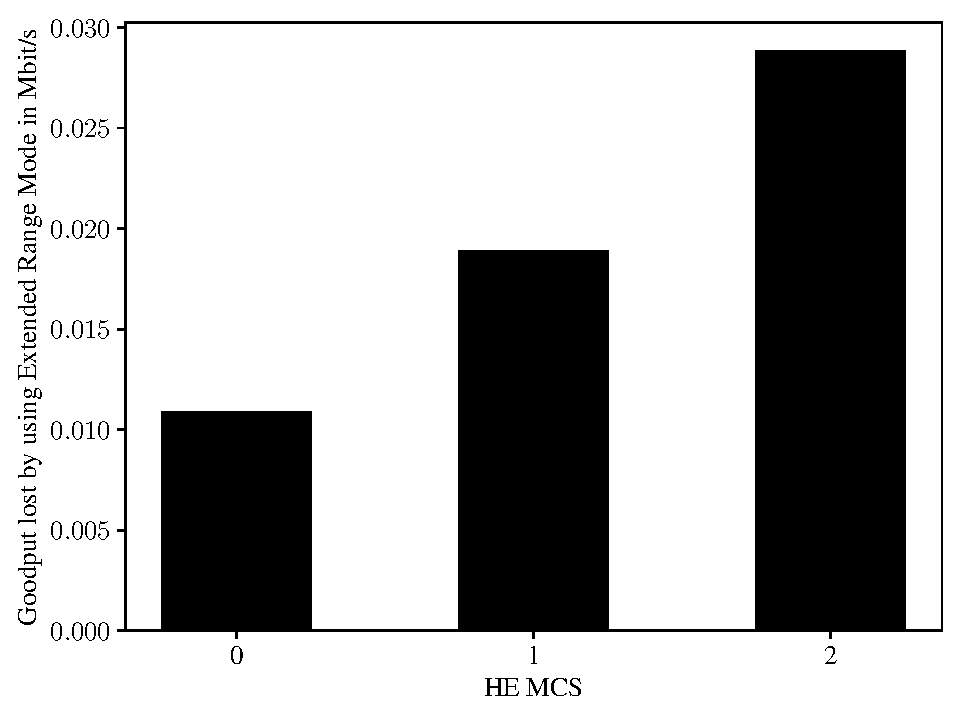
\includegraphics[width=0.64\textwidth]{figures/ER_dataRate_simulation.pdf}
   \caption{Lost Goodput between two Wi-Fi6 stations in Ad-Hoc Mode with a
   \acf{GI} of \SI{3200}{\nano\second} and a bandwidth of \SI{20}{\mega\hertz} in regards to \acf{HE}-\acf{MCS} when enabling the \ac{ER} mode}%
   \label{fig:Data_rate_ER}%
\end{figure}
The effect increases with smaller packet sizes because the longer preamble transmission time is more significant for smaller packets.
For higher \ac{HE}-\ac{MCS} values, more achievable goodput is lost because longer transmission time for the preamble could have
been used more \ac{OFDM} symbol transmissions, where more data is coded onto a symbol.

\subsubsection*{\acf{DCM}}
Using the \ac{DCM} in the IEEE 802.11ax physical layer also affects the achievable goodput.
As aforementioned, the \ac{DCM} is not supported by ns-3 version 3.37.
Therefore, I implemented the \ac{DCM} for this simulation in the ns-3 version 3.37 by transmitting a payload of twice the size, which represents the original payload and a
copy of it for the \ac{HE}-\ac{MCS} values 0, 1, 3 and 4, where \ac{MCS} is allowed.
Using \ac{DCM}, the receiver would apply maximum likelihood decoding to decode the original payload with a higher probability.

The results of the simulation are shown in \autoref{fig:Data_rate_DCM}, where the lost achieved goodput is plotted against
the theoretical data rate for the different \ac{HE}-\ac{MCS} values.
The theoretical data rate while using \ac{DCM} is half of the
theoretical data rate without \ac{DCM}, which complies with the IEEE 802.11ax standard \cite{ieee_standard_2021ax}.
\begin{figure}[H]%
   \centering
   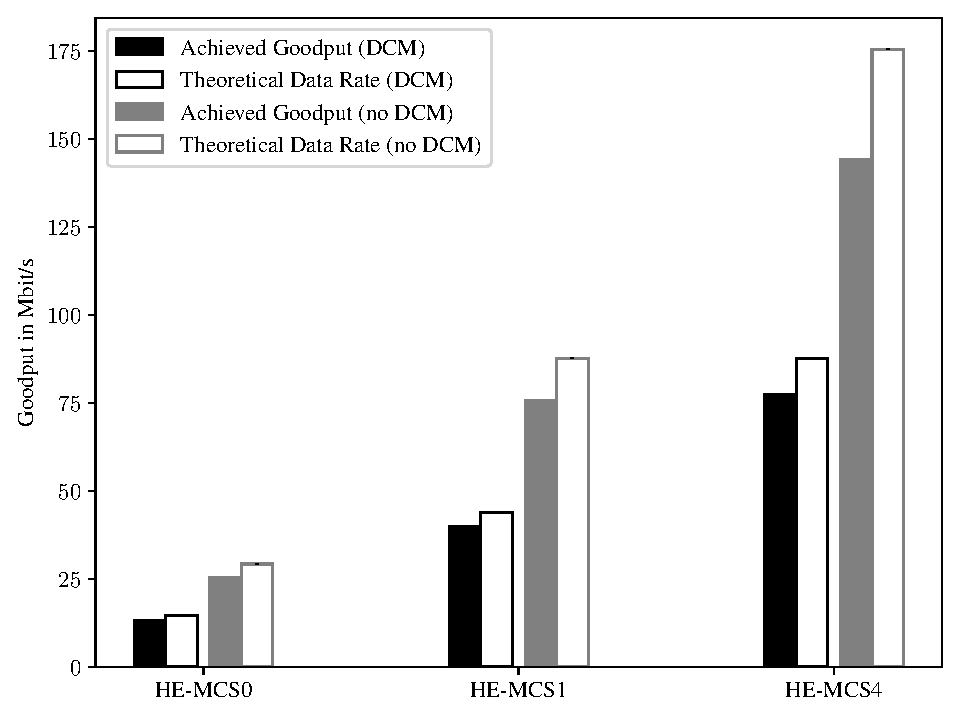
\includegraphics[width=0.64\textwidth]{figures/DCM_dataRate_simulation.pdf}
   \caption{Achieved Goodput and theoretical Datarate of two Wi-Fi6 stations in Ad-Hoc Mode with for IEEE 802.11ax physical layer parameters of a \acf{GI} of \SI{3200}{\nano\second}, a \acf{BW} of \SI{20}{\mega\hertz} and \num{2} spatial streams  in regards to the number of the chosen \ac{HE}-\acf{MCS} value and whether \acf{DCM} is enabled}%
   \label{fig:Data_rate_DCM}%
\end{figure}

The achieved goodput is always lower than the theoretical data rate because data transmission time is lost to the header overhead and media access time.
Wi-Fi access is based on \ac{CSMACA}, meaning the stations have to wait for a random time before transmitting on a free channel.
Additionally, the channel can be occupied by ACK or ad-hoc beacon frames, which must be transmitted.

Using \ac{DCM} increases the ratio of achievable goodput to theoretical data rate because only one header and one ACK frame are transmitted per
\SI{2000}{\byte} payload, and the node has to go to the medium access procedure only once per \SI{2000}{\byte} payload.


\begin{comment}
   sommer
   header_fixed  medium access (beacon, ACK, RTS, CTS) the achievable goodput is always lower than the theoretical data rate.
   theoretical data rate
\end{comment}




\subsubsection*{\acf{STBC}}
\label{sec:STBCDataRate}
Another physical layer parameter that reduces the theoretical data rate for more robustness is the \ac{STBC}.
As mentioned, ns-3 version 3.37 does not support the \ac{STBC} for the IEEE 802.11ax standard.
Therefore, I reduced the number of
\ac{MIMO} streams from \num{2} to \num{1} when the \ac{STBC} is enabled. \ac{STBC} would transmit a redundant copy of the data on the second antenna, which would be combined
using the space-time block code (STBC) to increase the robustness and reliability of the transmission.
The results of the simulation are shown in \autoref{fig:Data_rate_STBC}, where the lost achieved goodput is plotted against
the theoretical data rate for the different \ac{HE}-\ac{MCS} values.
The theoretical data rate while using \ac{STBC} is half of the theoretical data rate without \ac{STBC},
which complies with the IEEE 802.11ax standard \cite{ieee_standard_2021ax}.
\begin{figure}[H]%
   \centering
   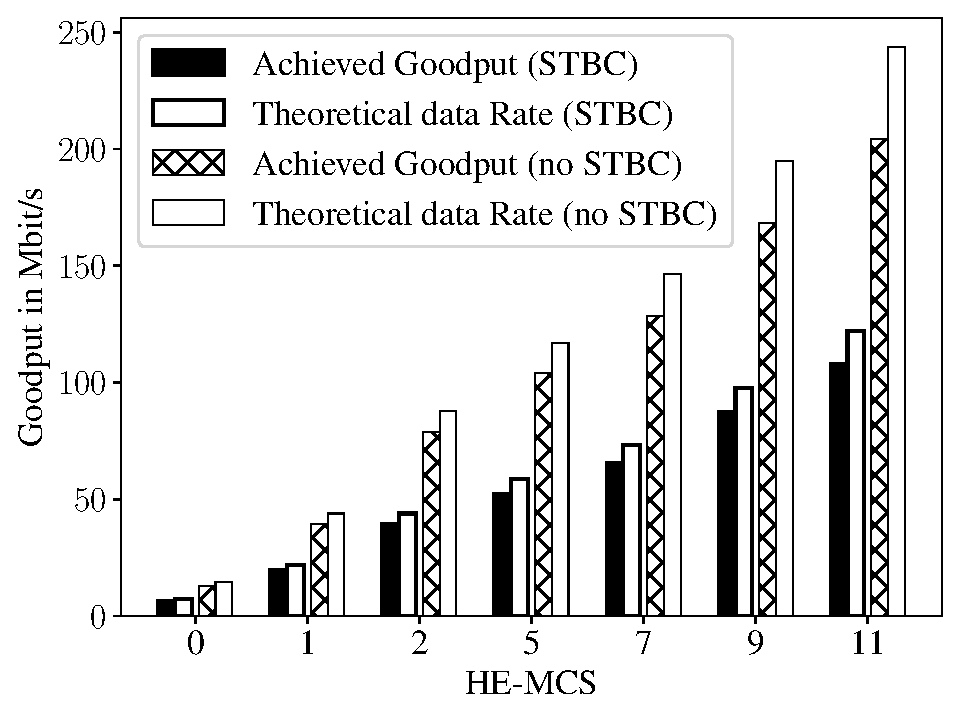
\includegraphics[width=0.64\textwidth]{figures/STBC_dataRate_simulation}
   \caption{Achieved Goodput and theoretical Datarate of two IEEE 802.11ax stations in Ad-Hoc Mode with for IEEE 802.11ax physical layer parameters of a \acf{GI} of \SI{3200}{\nano\second}, a \acf{BW} of \SI{20}{\mega\hertz} and 2 spatial streams  in regards to the number of the chosen \ac{HE}-\acf{MCS} value and whether \acf{STBC} is enabled}%
   \label{fig:Data_rate_STBC}%
\end{figure}

Other physical layer parameters, supported by the IEEE 802.11ax standard, are \ac{LDPC} and utilizing more \ac{MIMO} streams.
The effect that using more \ac{MIMO} streams for transmission increases the achievable goodput, is already known \cite[294-296]{sauter_wireless_2022, ieee_standard_2021ax, ieee_standard_2020}.
\ac{LDPC} adds no new effect for the achievable goodput, but more robustness which results in a lower \ac{PER}.

Using a different frequency spectrum, the achievable goodput can be limited due to the lower maximum \ac{BW} of \SI{40}{\mega\hertz} in the \SI{2.4}{\giga\hertz} frequency spectrum.
To analyze achievable goodput in the \SI{2.4}{\giga\hertz} frequency spectrum, I reran the simulations with the same configuration as in \autoref{sec:STBCDataRate}, but within the \SI{2.4}{\giga\hertz} frequency spectrum.
The results indicate that the achievable goodput is between \SIrange{0.1}{2.7}{\mega\bit\per\second} slower than in the \SI{5}{\giga\hertz} frequency spectrum.

Due to a signal extension of \SI{6}{\micro\second} in the \SI{2.4}{\giga\hertz} frequency spectrum, the transmission time is longer, which results in a lower achievable goodput.
\cite{ieee_standard_2009n} states that the signal extension in the \SI{2.4}{\giga\hertz} frequency spectrum enables
backwards compatibility with the older 802.11 standards, which need time to write their network allocation vector register.
\begin{comment}
\begin{figure}[H]%
   \centering
   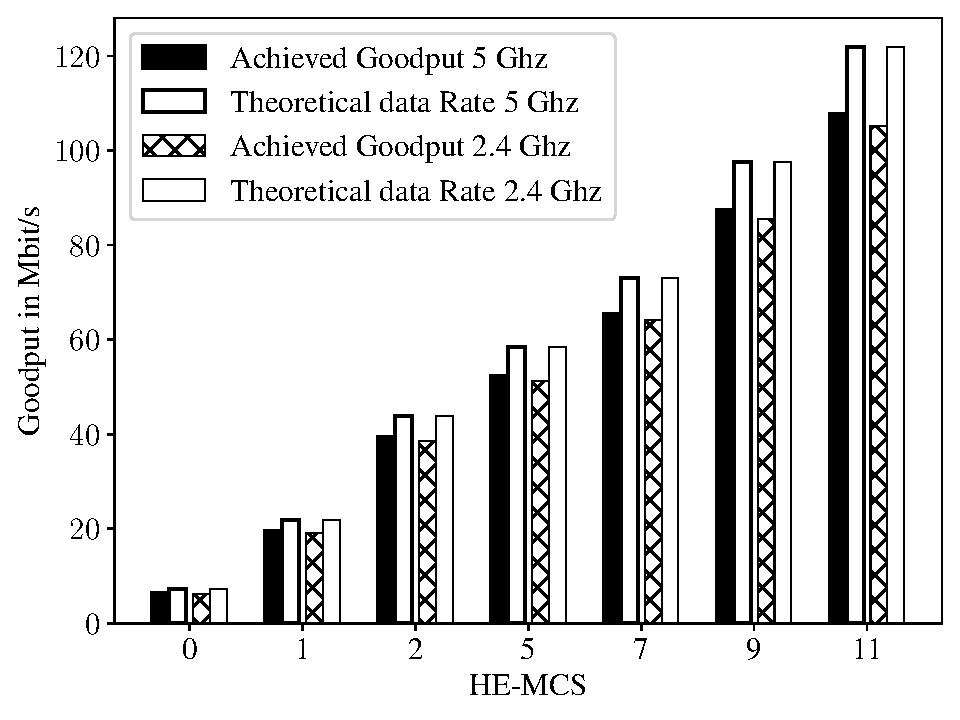
\includegraphics[width=0.95\textwidth]{figures/STBC_dataRate_simulation24}
   \caption{Achieved Goodput and theoretical Datarate of two IEEE 802.11ax stations in Ad-Hoc Mode with for IEEE 802.11ax
      physical layer parameters of a \acf{GI} of \SI{3200}{\nano\second}, a \acf{BW} of \SI{20}{\mega\hertz} and 2 spatial streams,
      \ac{STBC} enabled and in regards to the number of the chosen \ac{HE}-\acf{MCS} value and whether the
      \SI{2.4}{\giga\hertz} or \SI{5}{\giga\hertz} frequency spectrum is used}%
   \label{fig:Data_rate_STBC24}%
\end{figure}
\end{comment}

The simulation results represent an ideal scenario where only two nodes exchange data.
In a real-world scenario in the agricultural domain, the number of nodes and the distance between the nodes may be higher.
The signal propagation will be influenced by the complex agricultural environment,
which can consist of large water areas, various obstacles and vegetation or weather conditions \cite{brinkhoff_characterization_2017}.
In case of the corn harvest scenario, \textcite{smolnik_5g_2020} points out that corn plants can be up to \SI{3}{\metre} high
and thus influence signal propagation.
These factors in the real-world scenario can lead to higher \ac{PER} and thus reduce the achievable goodput.





\section{Link Level Simulation Evaluation}

The past two sections gave an overview of impact of the different parameters on the achievable goodput and robustness of the IEEE 802.11ax standard.
Both simulations were based on nearly ideal conditions, where the channel was not affected by any interference from other devices.

The results show the complex interplay of the different parameters in regards of the achievable goodput and robustness.
Every mentioned parameter can be set to have the highest possible data rate, which may lead to a low robustness and vice versa.
When the communication link is less robust, more retransmissions are required, which may result in a lower goodput.
When the configured data rate is too low, the goodput is also reduced.

As every application has different requirements on
latency, range, robustness and goodput, the parameters can be configured accordingly.

In general, modern Wi-Fi offer a variety of different parameters, to achieve the best possible performance for the specific application.
The new IEEE 802.11ax \ac{ER} mode combined with \ac{DCM} offers the highest robustness at low \ac{SNR}s according to my simulations, which can
be used for long range applications. The robustness simulation indicated, that the \ac{ER} mode and \ac{DCM} could extend the range, which was measured in the field experiment.

To deal with intersymbol interferences due to multipath effects, which were considered as the main reason for a high \ac{PER} in  Wi-Fi outdoor networks by
\cite{sheth_packet_2007} and \cite{aguayo_link-level_2004}, IEEE 802.11ax offers longer \ac{GI}s of up to \SI{3200}{\nano\second}.
My simulations show that \ac{GI} of \SI{3200}{\nano\second} is more robust against multipath effects than \ac{GI} of \SI{800}{\nano\second}, but
reduces the theoretical achievable data rate.

Since IEEE 802.11n, the robustness of the communication link can be increased by applying \ac{STBC}.
But just as the IEEE 802.11ax \ac{DCM} mode, the
increased robustness comes at the cost of a reduced theoretical data rate.

The following chapter analyses the impact of the different physical layer parameters on the latency of the Application Layer.

\chapter{Application Level Simulation}

\section{Agricultural Platooning Services}

After I analyzed the impact on data rate and robustness of the physical layer parameters, I will simulate a platooning scenario in ns-3 to find the influence of the physical layer configuration on the network performance.

The network performance metric consists of the latency, which describes the time needed to transmit the data
on the application layer, and the update rate of the platooning service, which defines how long ago a new position update
was received by the \ac{TM} in the Platooning Service.

Ns-3 is suitable for this simulation because it supports application layer-level simulation.
Via the extension Netsimulyzer, a graphical user interface is available to visualize the simulation results.

The simulation scenario is based on the corn harvest and loading scenario, which is described in \autoref{sec:corn_harvest_scenario}, where
multiple \acp{FH} harvest the corn and load it onto one of the \acp{TM}.

An ns-3 Node represents every machine.
Each Node has a mobility model, which describes the movement of the machine.

\subsubsection*{Wi-Fi Setup}
In order to exchange data between the machines, every machine is equipped with an  ns-3 IEEE 802.11ax WifiNetDevice.
Every Wi-Fi Device runs in Ad-Hoc mode to enable direct communication
between the machines.
The Wi-Fi data rate is managed by a Constant Rate Wi-Fi Manager, which has a non-unicast
transmission mode and a data mode for unicast transmissions.
The transmission modes are configured according
to the parameters in \autoref{tab:SimulationParametersWiFi}.

\begin{table}[H]
   \centering
   \begin{tabular}{p{6cm}p{4cm}}
      General Parameters & \\
      \midrule
      Wi-Fi Standard & IEEE 802.11ax\\
      \ac{GI} & \SI{3200}{\nano\second}\\
      \ac{LDPC} enabled & True\\
      Frequency Spectrum & \SI{5.6}{\giga\hertz}\\
      \ac{BW} & \SI{20}{\mega\hertz}\\
      Max. Transmission Power & \SI{25}{\decibel}\\
      Antenna Gain & \SI{5}{\dB}\\
      Maximum retries & \num{3}\\
       & \\
      Unicast Transmission Parameters & \\
      \midrule
      \ac{MCS} & \num{5}\\
      Number \ac{MIMO} Streams & \num{2}\\
       & \\
      Non-Unicast Transmission Parameters & \\
      \midrule
      Broadcast \ac{MCS} & \num{0}\\
      \ac{ER} mode enabled & True\\
      \ac{DCM} enabled & True\\
   \end{tabular}
   \caption{Default simulation parameters for Wi-Fi Devices on \acf{FH} and \acf{TM}}
   \label{tab:SimulationParametersWiFi}
\end{table}

The parameters are chosen from the results of the physical layer analysis of \autoref{sec:DataRate} and \autoref{sec:Robustness}.
Non-unicast transmissions are used to broadcast the Agricultural Platooning Service advertisements.

The non-unicast transmission parameters enable the longest possible
transmission range, which results in the lowest data rate.
Since no high data rate is required to advertise the Service, I chose the parameters to maximize the transmission range.
As aforementioned, ns-3 does not support \ac{DCM} at the moment.
In order to implement \ac{DCM} in the simulation, I doubled the data length for \ac{DCM} enabled transmissions to
represent the overhead of transmitting redundant copies of data for \ac{DCM}. \ac{DCM} would utilize the copies to determine the
correct data via maximum likelihood decoding.
As a result, the communication would be more robust, as shown in \autoref{sec:Robustness}.
This effect is not included in the current version of the simulation.

Guidance data in the Agricultural Platooning Service is exchanged between the \ac{FH} and the \ac{TM} via the
unicast transmission mode.
The process data in \autoref{chap:cornHarvestData} reflects that a short transmission range
is sufficient to exchange the guidance data, which must still be robust against multipath effects.
I chose the parameters to balance a high robustness and high data rate.
The unicast transmission parameters are changed in the simulation to analyze the impact on the network performance metrics.

Similar the ns-3 simulation in \autoref{sec:DataRate}, this simulation is based on the ns-3 ConstantSpeedPropagationDelayModel, the ns-3 FriisPropagationLossModel and
the ns-3 TableBasedErrorRateModel.


\subsubsection*{Agricultural Platooning Service}
Every machine node runs an ns-3 Application responsible for the Agricultural Platooning Service.
The application is identified by a unique identifier and runs a \ac{UDP} socket to exchange data with other Agricultural Platooning Service applications.
Every \ac{UDP} socket can be addressed by an IP address and a port number.
The IP address is the IP address of the machine node.

Throughout the simulation, I used ns-3 Packet Tags \footnote{\url{https://www.nsnam.org/docs/release/3.36/doxygen/classns3_1_1_tag.html}} to add information to packets that needed transferring between Agricultural Platooning Service applications.

Every \ac{FH} starts in the lower left corner of the field and harvests the corn along the path,
which is displayed in \autoref{fig:PlatooningRoute}.
As soon as a \ac{FH} reaches a field border, it makes a U-turn and continues
in the opposite direction.
Every \ac{FH} harvests the corn until it reaches the end of the field in the lower right corner.
The initial position of the \acp{TM} is a row below the \acp{FH}, which is displayed in \autoref{fig:PlatooningInit}.
\begin{figure}[H]%
   \centering
   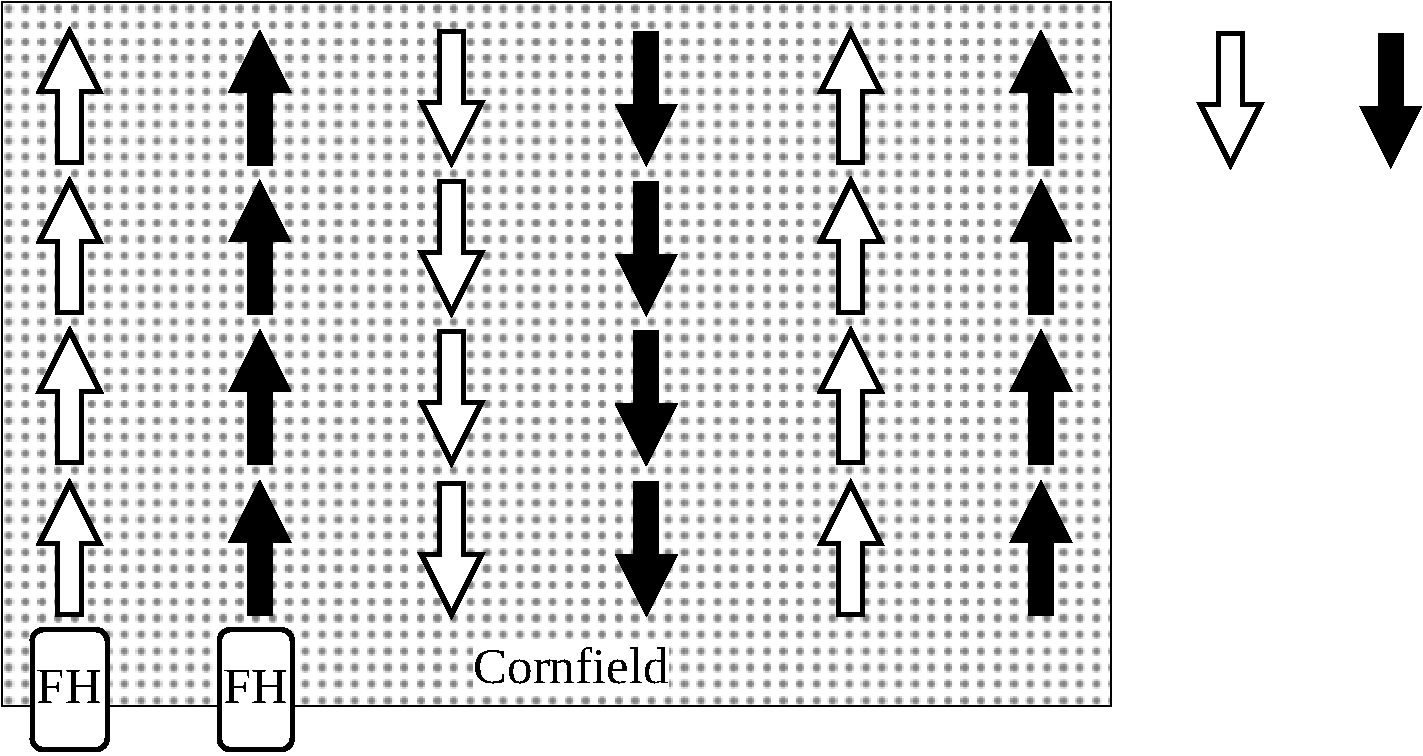
\includegraphics[width=0.7\textwidth]{figures/drawings-Route}
   \caption{Path of the \acf{FH} for harvesting corn on the field}
   \label{fig:PlatooningRoute}%
\end{figure}

In the beginning, every \ac{FH} broadcasts a search request $search\_TM$ via the non-unicast transmission mode to find an empty \ac{TM} to load the corn onto according to
to the procedure in \autoref{alg:SearchTM}.
As shown in \autoref{fig:PlatooningInit}, multiple \acp{TM} receive the search request and answer with
their current fill level of the \ac{TM}'s trailer.
The \ac{FH} chooses the \ac{TM} with the lowest fill level and sends a connection request to the \ac{TM}.
As soon as the \ac{TM} receives the connection request, it answers with a connection response.
When the \ac{FH} receives the connection response, the Agricultural Platooning Service is started.
When no \ac{TM} answers the search request, the \ac{FH} repeats the search request every $search\_TM\_interval$ seconds.

\begin{figure}[H]%
   \centering
   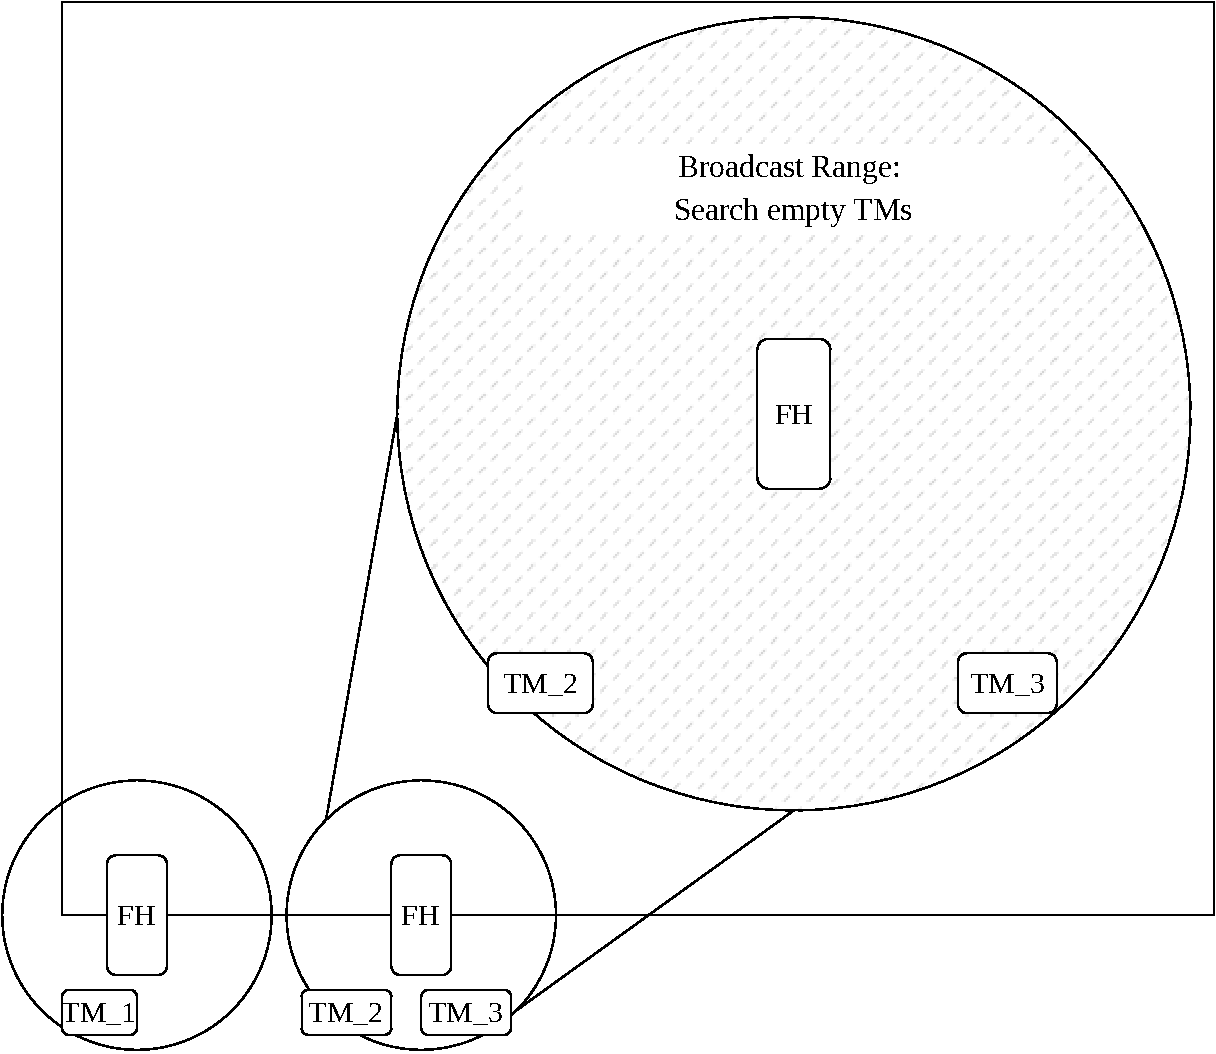
\includegraphics[width=0.83\textwidth]{figures/platoonINIT}
   \caption{Start position of the \acfp{FH} and \acfp{TM}, where a \ac{FH} broadcasts a search request to find
   a \ac{TM} to load the corn onto}
   \label{fig:PlatooningInit}%
\end{figure}

\begin{algorithm}
\begin{algorithmic}[1]
\REQUIRE Defined $search\_TM\_interval$, $search\_TM\_packet\_length$
\STATE Create packet $search\_TM$ of length $search\_TM\_packet\_length$ bytes
\STATE Broadcast $search\_TM$ to all \acp{TM}
\IF {no \acs{TM} ansers}
    \STATE Repeat Broadcasting $search\_TM$ every $search\_TM\_interval$ seconds
\ELSE
   \STATE Send connection request
   \IF {No \acs{TM} response}
      \STATE Repeat Broadcasting $search\_TM$ every $search\_TM\_interval$ seconds
   \ELSE
      \STATE Connection established
      \STATE Start Agricultural Platooning Service
   \ENDIF
\ENDIF
\end{algorithmic}
\caption{Procedure of the \acf{FH} to search for a \acf{TM} to load the corn onto}
\label{alg:SearchTM}
\end{algorithm}

Next, the \ac{FH} starts to harvest the corn.
All steps of the harvest process and Agricultural Platooning Service are summarized in
\autoref{alg:UpdateTM}.

\begin{algorithm}
\begin{algorithmic}[1]
\REQUIRE Defined $platoon\_data\_interval$, $platoon\_data\_packet\_length$
\STATE Calculate harvested volume
\STATE Advance \ac{FH} position
\STATE Add harvested volume to \ac{TM} fill level
\IF {\ac{TM} fill level is full}
    \STATE Disconnect from current \ac{TM}
	\STATE Start Agricultural Platooning Service with waiting \ac{TM}
\ELSE
	\STATE Create packet $TM\_data$ of length $platoon\_data\_packet\_length$ bytes, which contains the \ac{TM} fill level and the new guidance position
	\STATE Send $TM\_data$ to \ac{TM}
	\IF {\ac{TM} fill level is half full}
		\STATE Start \autoref{alg:SearchTM} to search for new \ac{TM}
	\ENDIF
\ENDIF
\end{algorithmic}
\caption{Procedure of the \acf{FH} to send the \acf{TM} fill level and the \ac{TM} guidance position every
\textit{platoon\_data\_interval}}.
\label{alg:UpdateTM}
\end{algorithm}

The FH harvest process is defined by the harvest states in \autoref{tab:harvestStatesDef},
where every harvest state represents a different \ac{PD} and \ac{FH} speed, which are derived from the key figures of a
\ac{FH} harvesting corn with a working width of \SI{6.2}{\meter} on a \SI{80}{\hectare} field in \cite{faustzahlen2018}.
When the \ac{PD} is low, the \ac{FH} can harvest faster and vice versa.

Starting in the harvest state H1, the \ac{FH} determines the next harvest state every \SI{50}{\milli\second}
by the Markov chain in \autoref{fig:MarkovChain}.
This Markov chain ensures that the harvest state can't transverse from H0 to H2 directly, which would represent
a low \ac{PD} immediately followed by a high \ac{PD}.
As I do not have enough harvest process data, which contain the \ac{PD} and the \ac{FH} speed,
I chose the transition probabilities to the best of my knowledge.
In future work, process data can be used to determine
the transition probabilities.

\begin{table}[H]
	\centering
	\begin{tabular}{>{\centering}p{2cm}p{4cm}p{4cm}}
		\toprule
		Harvest State & \ac{PD} & \ac{FH} speed\\
		\midrule
		H0 & \SI{20}{\tonne\per\hectare}
        & \SI{8.06}{\kilo\metre\per\hour} (\SI{2.24}{\metre\per\second}) \\
		H1 & \SI{30}{\tonne\per\hectare}
        & \SI{8.06}{\kilo\metre\per\hour} (\SI{2.24}{\metre\per\second}) \\
		H2 & \SI{50}{\tonne\per\hectare}
        & \SI{6.65}{\kilo\metre\per\hour} (\SI{1.845}{\metre\per\second}) \\
		\bottomrule
	\end{tabular}
	\caption{Corn harvest states, which define a range of \acfp{PD} and \acf{FH} speeds, where the data is derived from
	key figures \cite{faustzahlen2018}}
	\label{tab:harvestStatesDef}
\end{table}

\begin{figure}[H]
\centering
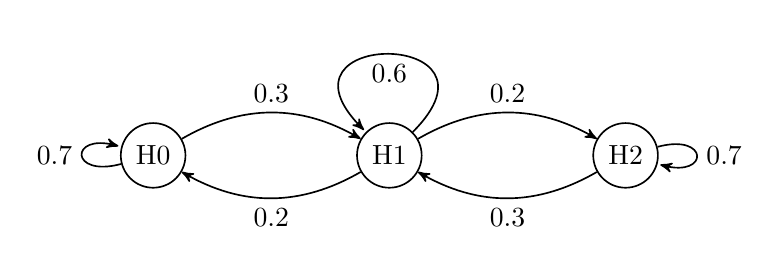
\begin{tikzpicture}[->, >=stealth', auto, semithick, node distance=3cm]
	\tikzstyle{every state}=[fill=white,draw=black,thick,text=black,scale=1]
    \node[circle, draw]    (A)               {H0};
	\node[circle, draw]    (B)[right of=A]   {H1};
	\node[circle, draw]    (C)[right of=B]   {H2};
	\path
	(A) edge[loop left]			node{0.7}	(A)
        edge[bend left,above]	node{0.3}	(B)
	(B) edge[bend left,below]	node{0.2}	(A)
        edge[bend left,above]   node{0.2}	(C)
        edge[loop]		        node{0.6}	(B)
	(C) edge[bend left,below]	node{0.3}	(B)
        edge[loop right]		node{0.7}	(C);
	\end{tikzpicture}
\caption{Markov Chain for the Harvest States 0, 1 and 2, which represent the current \ac{PD} and
harvest speed from \autoref{tab:harvestStatesDef}}
\label{fig:MarkovChain}
\end{figure}

After determining the next harvest state, the \ac{FH} sets the \ac{PD} and the \ac{FH} speed according to the defined values in
\autoref{tab:harvestStatesDef}.
The position of the \ac{FH} is advanced by the \ac{FH} speed multiplied with \SI{50}{\milli\second} along the
harvest path in \autoref{fig:PlatooningRoute}.
The harvested volume during this $platoon\_data\_interval$ is calculated with the following
equations:
\begin{equation}
   \label{eq:AreaCalculation}
   \text{Harvested Area} =
      \text{Harvest width} \times \text{Harvest speed} \times \text{Time step}
   ,
\end{equation}
\begin{equation}
   \label{eq:VolumneCalculation}
   \text{Harvested Volume} =
   \text{Harvested Area} \times \text{\ac{PD}} \times \text{Corn volume per tonne}.
\end{equation}

The harvested area is represented in \si{\hectare}, and
the harvested volume is defined in \si{\cubic\metre}.
The needed parameters for the calculation are from \cite{faustzahlen2018} and are listed in \autoref{tab:SimulationParameters}.
The calculated harvested volume is added to the \ac{TM}'s fill level, which is tracked by the \ac{FH}'s application.
Keeping track of the fill level represents the knowledge of the \ac{FH} about the \ac{TM}'s fill level, which the \ac{FH} would
normally get through a sprout guidance system.

Next, the \ac{FH} determines whether the \ac{TM} is full.
If the \ac{TM} is full, the \ac{FH} stops harvesting and sends a disconnect request to the \ac{TM}.
The \ac{TM} answers with a disconnect response and leaves the field to unload the corn, as shown in \autoref{fig:PlatooningFull}.



If the \ac{TM} is not full, the \ac{FH} sends the $TM\_data$ to the \ac{TM},
which contains the new \ac{TM} fill level and the new guidance position.
The \ac{TM} updates the fill level and drives to the new position to load the corn, as shown in \autoref{fig:PlatooningHF}.
The guidance data positions the \ac{TM} always \SI{5}{\metre} left of the \ac{FH} because this part of the field was already harvested.
The distance between the \ac{FH} and the \ac{TM} is  as the \ac{FH} and the \ac{TM} moved mostly with a distance of around \SI{5}{\metre} in
the recorded process data in \autoref{chap:cornHarvestData}.

\begin{figure}[]%
	\centering
	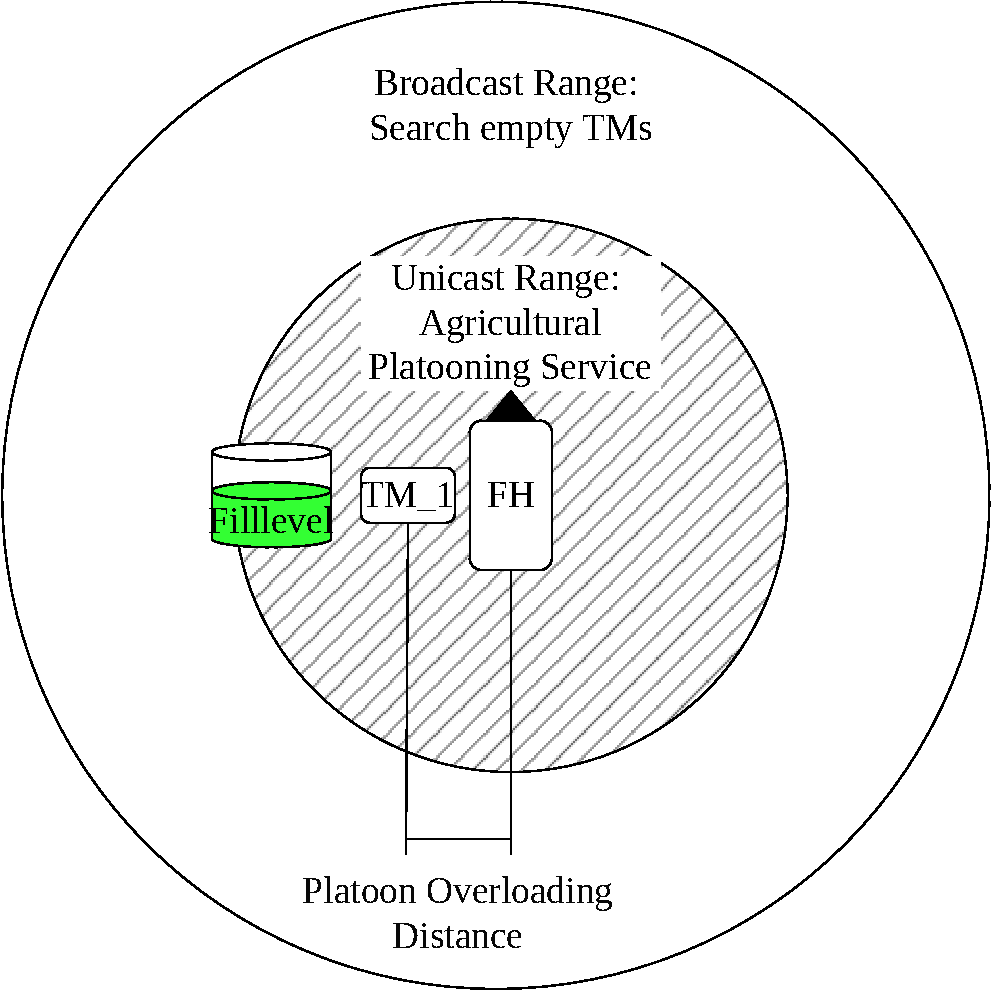
\includegraphics[width=0.65\textwidth]{figures/platoonHALF}
	\caption{\acf{TM} position left of the \acf{FH} for overloading, where the \ac{TM} is half full and the
		\ac{FH} starts \autoref{alg:SearchTM} to search for a next empty \ac{TM},
		which can later take over the loading position.}
	\label{fig:PlatooningHF}%
\end{figure}
If the \ac{TM} fill level is half full, the \ac{FH} starts \autoref{alg:SearchTM}
to search for a new \ac{TM} to load the corn onto.
This process is visualized in \autoref{fig:PlatooningHF}.
As soon as the \ac{FH} finds a new \ac{TM}, the \ac{FH} connects to the new \ac{TM} and starts sending
the \ac{TM} guidance positions, which place the \ac{TM} \SI{12}{\metre} behind the \ac{FH}.
The \ac{FH} continues harvesting until the \ac{TM} is fully loaded.
Meanwhile, the new \ac{TM} is waiting behind the \ac{FH} and can take over the loading position next to the \ac{FH} as
soon as the \ac{TM}, where the \ac{FH} is currently loading onto, is full.

\begin{figure}[]%
	\centering
	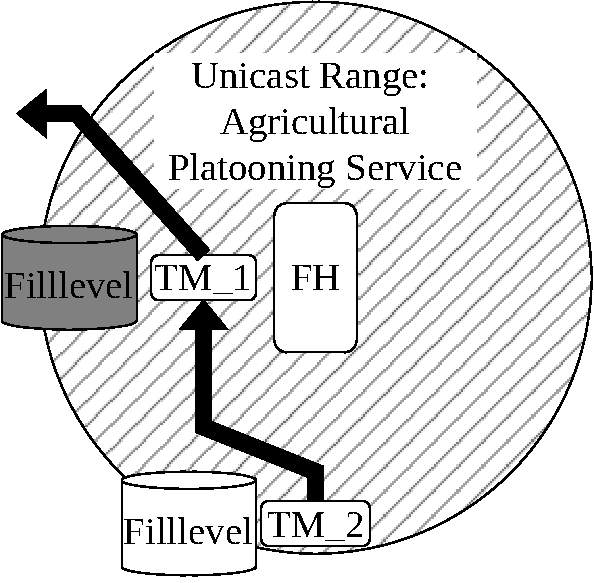
\includegraphics[width=0.39\textwidth]{figures/platoonFULL}
	\caption{Change of \acfp{TM} in the Application Agricultural Platooning Service, where $TM\_1$
	is full and leaves the field while the empty $TM\_2$ takes over the overloading position.}
	\label{fig:PlatooningFull}%
\end{figure}

A fully loaded \ac{TM} leaves the field to unload the corn and returns to the position where it disconnected from the \ac{FH}.
There, it waits for an incoming $search\_TM$ request from a \ac{FH} to connect to a \ac{FH} again.

The corn harvest process is finished when the last \ac{FH} has finished harvesting and moved to the end of the field as
shown in \autoref{fig:PlatooningRoute}.

\begin{table}[H]
	\centering
	\begin{tabular}{p{5cm}p{4cm}}
		\toprule
		Parameters & \\
		\midrule
		\textit{search\_TM\_interval} & \SI{1}{\second}\\
		\textit{search\_TM\_packet\_length} & \SI{0.5}{\kilo\byte}\\
		\textit{platoon\_data\_interval} & \SI{50}{\milli\second}\\
		\textit{platoon\_data\_packet\_length} & \SI{1}{\kilo\byte}\\
		Platoon Overloading Distance & \SI{5}{\meter}\\
		\ac{FH} Working Width & \SI{6.2}{\meter}\\
		\ac{TM} Volume & \SI{50}{\cubic\meter}\\
		\bottomrule
	\end{tabular}
	\caption{Simulation parameters for the Application Agricultural Platooning Service}
	\label{tab:SimulationParameters}
\end{table}

\subsubsection*{Simulation Verification}
Each corn harvest scenario is visualized to ensure the correctness of the simulation.
The visualizations are created with the ns-3 extension Netsimulyzer.
The corn field is marked as a black rectangle. Next to the lower left corner there is a cuboid which marks the location of the silo.
Every node was displayed as the Netsimulyzer model of a landdrone, where all \acp{FH} are black and the
\acp{TM} are either red, green, yellow or blue, depending on the \ac{TM} state.
\begin{figure}[H]%
	\centering
	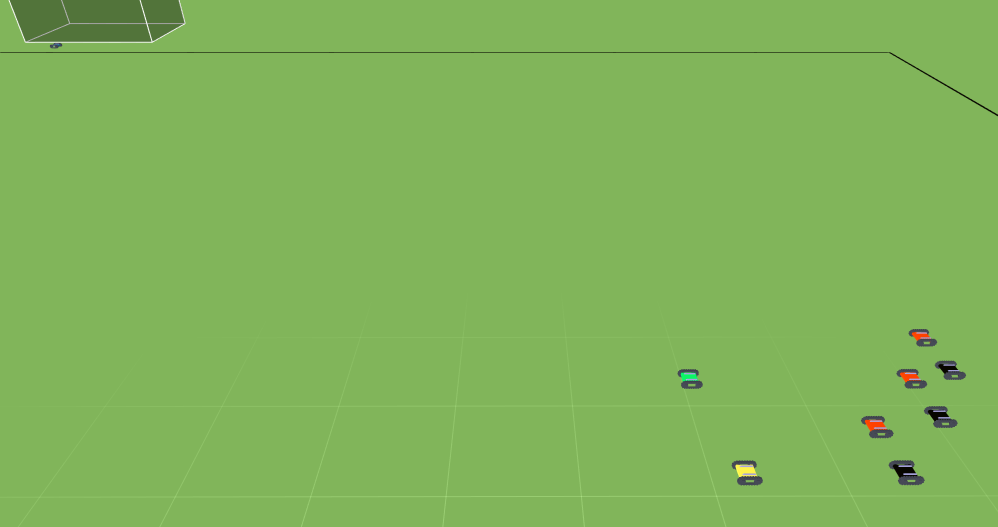
\includegraphics[width=0.75\textwidth]{figures/platooningScreen}
	\caption{Screenshot of the simulation visualization in Netsimulyzer, where a blue \acf{TM} is unloading in the back in front of the farm cuboid,
		two red \acp{TM} are in a Agricultural Platooning Service with the black \acfp{FH},
		a green \ac{TM} is empty and waiting for a new $search\_TM$ request and a yellow \ac{TM} is in waiting position behind a black \ac{FH}.}
	\label{fig:PlatooningScreenshot}%
\end{figure}

An empty \ac{TM} is displayed green and changes to yellow as soon as it is associated with a \ac{FH} and in waiting position behind the \ac{FH}.
The \ac{TM} is red as soon as the \ac{FH} starts loading the corn onto the \ac{TM} in an Agricultural Platooning Service.
A full \ac{TM} is displayed blue and moves to the farm cuboid next to the lower left corner of the field.
As soon as the \ac{TM} is empty, it changes back to green and waits for a new \ac{FH} to connect to it at the last disconnection position.

I use this visualization to verify the correct mobility of the \ac{FH} and the \ac{TM}, the correct \ac{TM} state transitions,
that the simulation is ending properly and that the \ac{FH} switches the waiting \ac{TM} after disconnecting
from the fully loaded \ac{TM}.

Using the provided information from the ns-3 MonitorSnifferRxCallback and MonitorSnifferTxCallback I was able to review ongoing transmissions and
whether the specified physical layer parameters are used correctly for non-unicast and unicast traffic.

Every simulation runs \num{2} \acp{TM} per \ac{FH}.
This does not correspond to the key figures of 10 \acp{TM} per \ac{FH} in the corn harvest scenario \cite{faustzahlen2018},
but is sufficient as there is no communication of \acp{TM} while transporting the harvested crop to the farm currently planned.
For this reason, I have set the simulation so that a full \ac{TM} is empty again after \SI{10}{\second} at the disconnect position.
This is a reasonable value, as it ensures that every time a \ac{FH} starts a $search\_TM$ request, there is a \ac{TM} in range to connect to.

\textcite{zhang_method_2009} defined a data frame of \SI{32}{\byte}, which includes an identifier, timestamp, longitude,
latitude, heading, speed and direction.
This set of data comprises a basic set which is sufficient for the implementation of a platooning service,
as the authors show.
\textcite{schlingmann_aef_2019} do not specify the amount of data further and point out that the required data rate
for platooning services is low.

The use case requirements for vehicle platooning services in \cite{TR-22.886} specify data sizes of \SIrange{300}{1200}{\kilo\byte},
depending on the vehicle density.

I have set the data size \textit{platoon\_data\_packet\_length} to \SI{1}{\kilo\byte} for the simulation of platooning services.
This data size is an abstraction of the storage space that may be needed for additional data or implementations
of authentication and security mechanisms.
In the Corn Harvest scenario, additional data could be, for example, the fill level of the transport machine,
information about the environment, obstacles or other machines on the field.

\textcite{zhang_method_2009} already showed that an interval of \SI{100}{\milli\second} is sufficient for Agricultural Platooning Services
in a harvest scenario.

I chose a $platoon\_data\_interval$ of \SI{50}{\milli\second} for the Agricultural Platooning Service
as \textcite{smolnik_5g_2020} mention that their requirements analysis indicated that new guidance data should at least arrive every \SI{50}{\milli\second}.

\section{Application Level Simulation Evaluation}
I chose the following simulation configurations for the unicast transmission of guidance data: \ac{HE}-\ac{MCS} 3, 5 and 7 and
\ac{STBC} either enabled or disabled.
Every simulation configuration runs \num{5} times, where every \ac{FH} harvests \SI{1}{\hectare} of corn, which equals to roughly
\num{2.5} \ac{TM} loads.
Every simulation run has a different random seed.
After the simulation run successfully and the simulation process is verified in the visualization,
a mean value and confidence interval with a confidence level of
\SI{95}{\percent} is calculated per simulation configuration.

The results for defined metrics latency and data update rate are shown in \autoref{fig:mean_50}.


\begin{figure}[]%
	\centering
	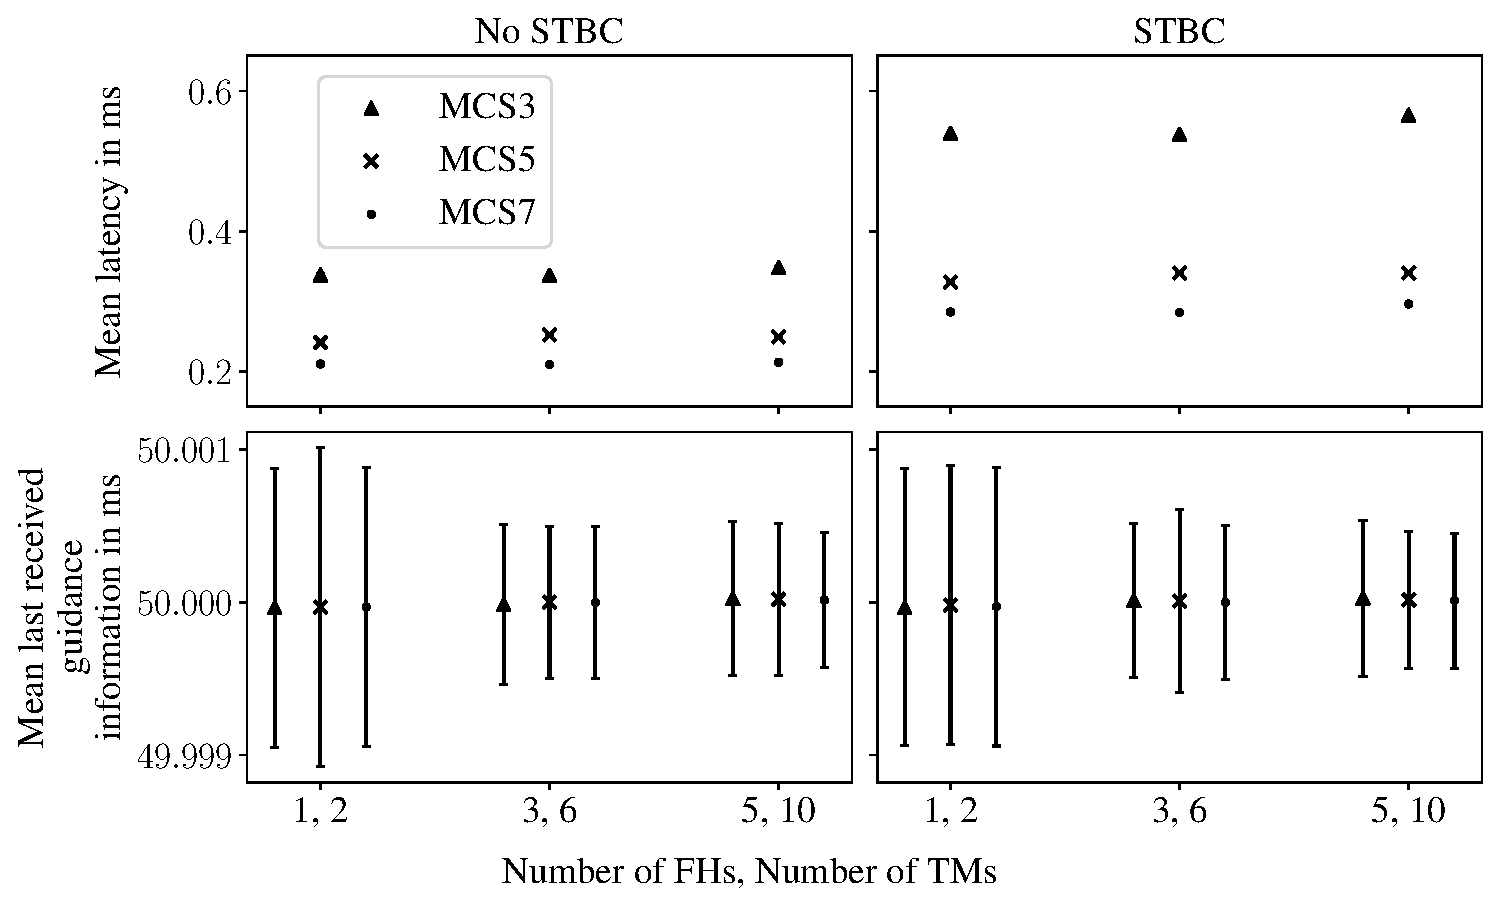
\includegraphics[width=0.98\textwidth]{figures/latency_lastUpdate50ms}
	\caption{Mean latency and mean guidance data update interval of the Application Agricultural Platooning Service
	in regards to the number of \acfp{FH} and \acfp{TM}, enabled \ac{STBC} and
	the chosen \ac{HE}-\ac{MCS} value for a $platoon\_data\_interval$ of \SI{50}{\milli\second}.}
	\label{fig:mean_50}%
\end{figure}

The desired $platoon\_data\_interval$ of \SI{50}{\milli\second} can be achieved with every
configuration.

The confidence interval for the mean update rate is always below \SI{2}{\micro\second}.
The mean latency is always below \SI{0.6}{\milli\second}.
Using higher \ac{HE}-\ac{MCS} values significantly reduces the mean latency of
the Agricultural Platooning Service data exchange.

Applying \ac{STBC} additionally increases the mean latency compared to
non- \ac{STBC} configurations.
This is due to the fact that the \ac{STBC} configuration uses the redundant copy of data to
improve the reliability of the transmission by applying maximum likelihood decoding.
This decreases the data rate and increases
the mean latency.
Nevertheless, the desired $platoon\_data\_interval$ of \SI{50}{\milli\second} can be achieved when using \ac{STBC} for
every specified \ac{HE}-\ac{MCS} value and thereby increase the reliability of the transmission.

The recorded process data from the corn harvest scenario showed that the \ac{FH} can also harvest at higher speeds around
\SI{10}{\kilo\meter\per\hour} than can be calculated from the key figures in \cite{faustzahlen2018}.
To test the applicability of the Agricultural Platooning Service for higher speeds, I ran a additional simulation where I changed the
harvest states according to \autoref{tab:harvestStatesChanged}.

\begin{table}[H]
	\centering
	\begin{tabular}{>{\centering}p{2cm}p{4cm}p{4cm}}
		\toprule
		Harvest State & \ac{PD} & \ac{FH} speed\\
		\midrule
		H0 & \SI{20}{\tonne\per\hectare}
        & \SI{14}{\kilo\metre\per\hour} (\SI{3.89}{\metre\per\second}) \\
		H1 & \SI{30}{\tonne\per\hectare}
        & \SI{12}{\kilo\metre\per\hour} (\SI{3.33}{\metre\per\second}) \\
		H2 & \SI{50}{\tonne\per\hectare}
        & \SI{10}{\kilo\metre\per\hour} (\SI{2.78}{\metre\per\second}) \\
		\bottomrule
	\end{tabular}
	\caption{Corn harvest states, which define a range of \acfp{PD} from \cite{faustzahlen2018} and \acf{FH} speeds,
	which I set higher than the key figures in \cite{faustzahlen2018} specify to
	increase the requirements on the Agricultural Platooning Service.}
	\label{tab:harvestStatesChanged}
\end{table}

As I increased the \ac{FH} speed, which leads each harvest platoon, the whole platoon harvests the field faster.
Therefore, all \acp{TM} move faster.
To provide faster \acp{TM} more often with guidance data,
I decreased the $platoon\_data\_interval$ to \SI{25}{\milli\second} to ensure,
that a \ac{TM} always stays in the harvest platoon position even at higher speeds.

This $platoon\_data\_interval$ of \SI{25}{\milli\second} heads in the direction of the upper required update rate of \SIrange{10}{25}{\milli\second} for general
vehicle platooning services in \cite{TR-22.886}.
But the values in \cite{TR-22.886} correspond to higher platoon sizes, a velocity of \SI{100}{\kilo\meter\per\hour} and a
vehicle distance of \SIrange{1}{2}{\metre}.


\begin{figure}[]%
   \centering
   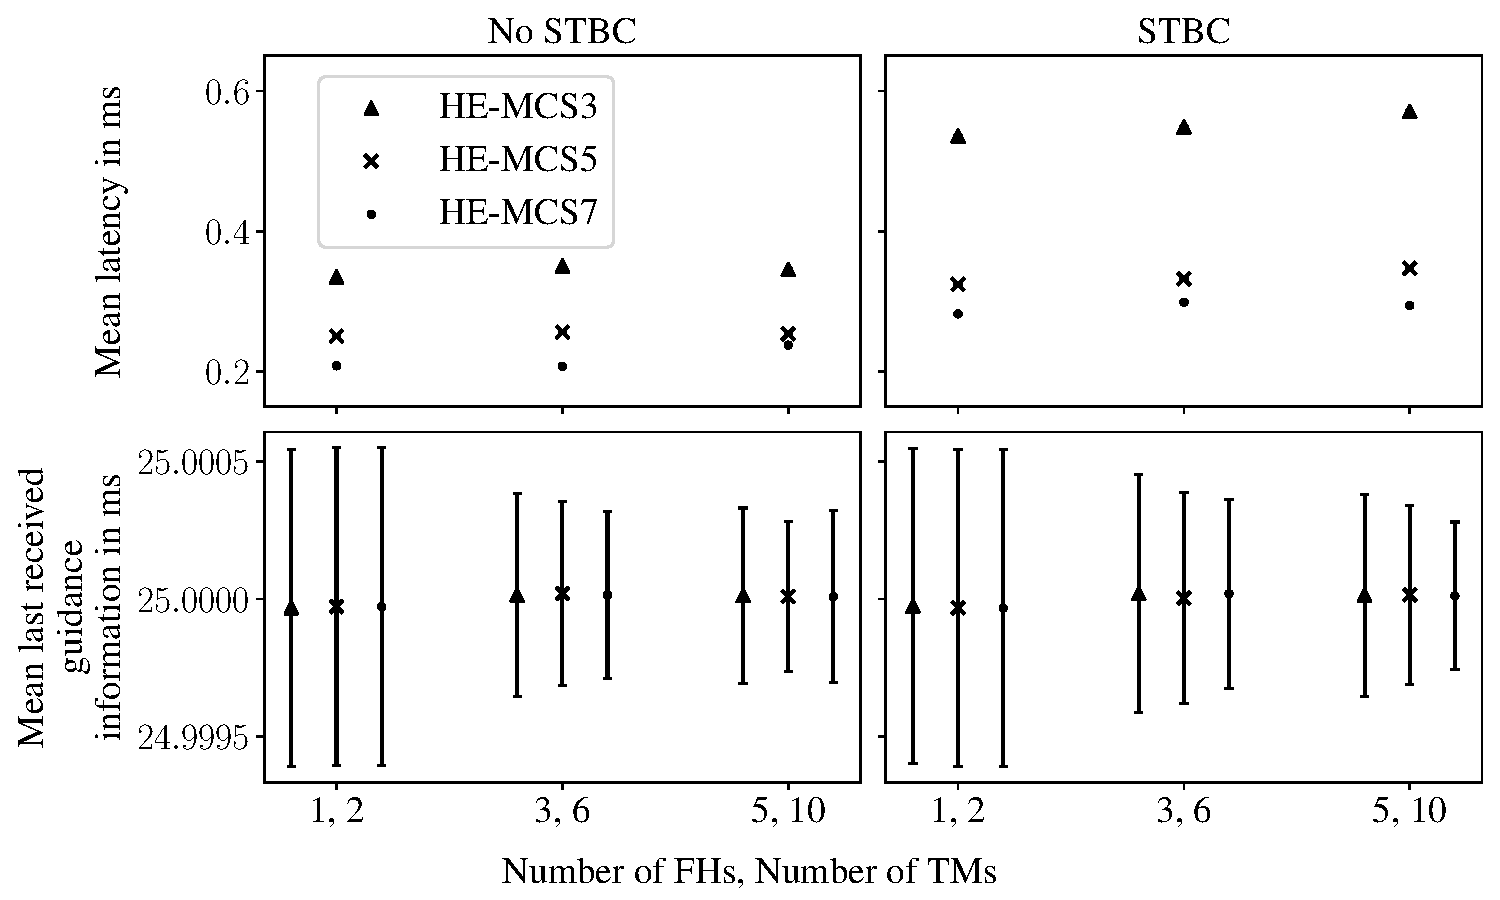
\includegraphics[width=0.98\textwidth]{figures/latency_lastUpdate25ms}
   \caption{Similar to \autoref{fig:mean_50}, mean latency and mean guidance data update interval of the Application Agricultural Platooning Service
   with the same configuration are shown but for a different $platoon\_data\_interval$ of \SI{25}{\milli\second}.}
   \label{fig:mean_25}%
\end{figure}

The simulation runs with the same physical layer configurations as in \autoref{fig:mean_50}.
The results displayed in \autoref{fig:mean_25} reveal that the mean guidance data update interval is always around \SI{25}{\milli\second},
which is the desired $platoon\_data\_interval$.
The mean latency is nearly the same as in \autoref{fig:mean_50}, which indicates that there is still some channel capacity left for
further data exchange.
Again, as the number of \acp{TM} and \acp{FH} increases, the mean latency increases slightly.

Both simulations were based on the abstracted and simplified corn harvest scenario, which is based on the ns-3 communication model and
abstracted implementation of the physical layer and MAC layer in ns-3.
In a real-world scenario, an Agricultural Platooning Service has to operate in the complex agricultural environment, which
may impact signal propagation and communication performance.

The simulated communication is based on a \ac{BW} of \SI{20}{\mega\hertz}, which offers the highest possible signal power spectral density.
Additional robustness is gained by using \ac{STBC}, \ac{LDPC}, low \ac{MCS} values and \ac{CR}s which are encoded for example in
\ac{HE}-\ac{MCS}3 and are available since the IEEE 802.11n standard.
These physical layer configurations are enough to transmit guidance data in an Agricultural Platooning Service.

Both simulations did not consider the impact of interference due to other ongoing transmissions.
For example, \ac{WIC} Video streaming services can increase the network load and consequently lead in higher latencies for
the Agricultural Platooning Service.
A solution would be to prioritize the Agricultural Platooning Service over other services
to ensure a certain quality of service.
When passing houses, industrial, or farm buildings, additional Wi-Fi transmissions can be expected.
Interference with other Wi-Fi
transmissions can easily occur, when the channel is heavily loaded.
The results showed that some channel capacity is still left for further data exchange of other channel users.
Since a narrow bandwidth of \SI{20}{\mega\hertz} is used, interference is less likely compared to wider bandwidths,
as a wider spectrum is likely to be more utilized if transmission in the frequency spectrum are equally distributed.


Using IEEE 802.11ax, a new service discovery transmission mode is available.
Additionally, to the lowest \ac{MCS} and \ac{CR},
IEEE 802.11ax can apply the \ac{ER} mode with \ac{DCM} which increases robustness as shown in \autoref{sec:Robustness}
and therefore increases the communication range.
This physical layer amendment is designed to introduce a new level of long-range communication in IEEE 802.11.
At the moment, I am not aware of any research that measured the resulting communication range in an agricultural environment.

If the communication range is not sufficient for service discovery, a road side unit at the field entrance can be used to exchange \ac{FH} position data
between \acp{TM} leaving and entering the field.
Alternatively, a field planner can be used to give an overview of where a \ac{FH} should be harvesting,
when everything works as expected.
These two options can provide \ac{FH} position estimations, which can be used to guide \acp{TM} to a position where they are likely
to receive service discovery broadcasts from \acp{FH}.








\begin{comment}
	\chapter{Evaluation}


\begin{itemize}
\item measurement setup / results / evaluation / discussion
\item whatever you have done, you must comment it, compare it to other systems, evaluate it
\item usually, adequate graphs help to show the benefits of your approach
\item each result/graph must not only be described, but also discussed (What's the reason for this peak? Why have you observed this effect? What does this tell about your architecture/system/implementation?)
\item recommended length: approximately one third of the thesis.
\end{itemize}
\end{comment}



\chapter{Conclusion}
\acresetall
\begin{comment}
    \begin{itemize}
    \item summarize again what your paper did, but now emphasize more the results, and comparisons
    \item write conclusions that can be drawn from the results found and the discussion presented in the paper
    \item future work (be very brief, explain what, but not much how, do not speculate about results or impact)
    \item recommended length: one page.
    \end{itemize}
\end{comment}
This thesis investigates the suitability of modern Wi-Fi for \ac{WIC}, which describes a wireless process data exchange between agricultural machines in the field.
The investigation is based on the prototypical application Agricultural Platooning Service in the corn harvest scenario, which exchanges guidance data via \ac{WIC} to lead \acp{TM} to the overloading positions of forage from \acp{FH}.

I analyzed corn harvest process data, which indicated that the overloading position is usually at a distance below \SI{10}{\metre} at every angle relative to the \ac{FH}.

A field measurement campaign in a farming environment indicated Wi-Fi communication can range up to \SI{2500}{\metre} in a line-of-sight scenario.
However, signal strength can suffer from multipath, shadowing and fading effects due to the agricultural environment and the machine sizes.
Therefore, Wi-Fi rate managers should be configured to enable robust communication instead of maximizing the data rate.

I simulated different Wi-Fi physical layer configurations to analyze their impact on data rate and robustness.
IEEE 802.11ax introduces the new \ac{ER} mode, enabling robust and long-range communication for service discovery transmission when used with \ac{DCM}.
The \ac{GI} of \SI{3.2}{\micro\second} in IEEE 802.11ax can be used to combat intersymbol interferences due to multipath effects in the agricultural environment.
The guidance data exchange mode can be configured to use low \acp{MCS} like \ac{HE}-\ac{MCS}3 with \ac{STBC} and \ac{LDPC} to achieve a robust communication,
which enables the \ac{WIC} to meet the required latencies and message intervals for Agricultural Platooning Services in the corn harvest scenario.

In this thesis, I showed that IEEE 802.11ax provides many configurations to enable robust communications which meet the requirements of the use case Agricultural Platooning Services.



\begin{comment}
    Untersuchen, welche Routing protocols
    Wi-Fi offers a wide range of physical layer configurations, which can be used to reduce the data rate and enable robust communication.

    Future work could investigate whether modern Wi-Fi can be used for other \ac{WIC} use cases.
    IEEE 802.11bd is a new standard, which is designed for \ac{WIC} in the industrial domain.


    Guten Tag Herr Professor Sommer,

Anbei finden Sie die aktuelle Version meiner Diplomarbeit, welche nun auch die Feldversuche enthält. Wenn Sie noch nicht auf die Diplomarbeit schauen konnten oder noch vor Kapitel 4 Field Measurements sind, können Sie gerne auf die aktuelle Version im Anhang wechseln.

Die PDF musste ich komprimieren, weil sie sonst zu groß war. Wenn Sie eine unkomprimierte Version lieber wollen, kann ich ihnen gerne einen Zugang zum Git-Repro geben.

Vielen Dank,

Karl Lautenschläger
\end{comment}

\cleardoublepage

\listofabbreviations
\clearpage

\listoffigures
\clearpage

\listoftables
\clearpage

\printbibliography

\end{document}
